\subsection{Gallery of DOS/PDOS}
We first present our spectral histogram approximation from DOS/ PDOS on a wide
variety of graphs, including collaboration networks, online social networks,
road networks and autonomous systems (dataset details are in the appendix). For
all examples, we apply our methods to the normalized adjacency matrices using
$500$ Chebyshev moments and $20$ Hadamard probe vectors. Afterwards, the
spectral density is integrated into $50$ histogram bins. In \cref{fig:gallery},
the DOS approximation is on the first row, and the PDOS approximation is on the
second. When a spike exists in the spectrum, we apply motif filtering, and DOS
is zoomed appropriately to show the remaining part. For PDOS, we stack the
spectral histograms for all nodes vertically, sorted by their projected weights
on the leading left singular vector. Red indicates that a node has high weight
at certain parts of the spectrum, whereas blue indicates low weight.

We observe many distinct shapes of spectrum in our examples. The eigenvalues of
denser graphs, such as the Marvel characters network (\ref{fig:marvel_ldos}:
average degree $52.16$) and Facebook union of ego networks 
(\ref{fig:facebook_ldos}: average degree $43.69$), exhibit decay similar to
thepower-law around $\lambda=0$. There has been study on the power-law
distribution in the eigenvalues of the adjacency and the Laplacian matrix, but
it only focuses on the leading eigenvalues rather than the entire spectrum~
\cite{eikmeier2017revisiting} for large real-world datasets. Relatively sparse
graphs (\ref{fig:erdos_ldos}: average degree $3.06$,; \ref{fig:as_ldos}: average
degree $4.13$) often possess spikes, especially around $\lambda=0$, which
reflect a larger set of loosely-connected boundary nodes. It is much more
evident in the PDOS spectral histograms, which allow us to pick out the nodes
with dominant weights at $\lambda=0$ and those that contribute most to local
structures. Finally, though the road network is quite sparse (ave. deg $2.50$),
its regularity results in a lack of special features, and most nodes contribute
evenly to the spectrum according to PDOS.

\begin{figure}[htp]
  \begin{subfigure}[t]{0.19\textwidth}
    \centering  
    \captionsetup{justification=centering,font=scriptsize}
    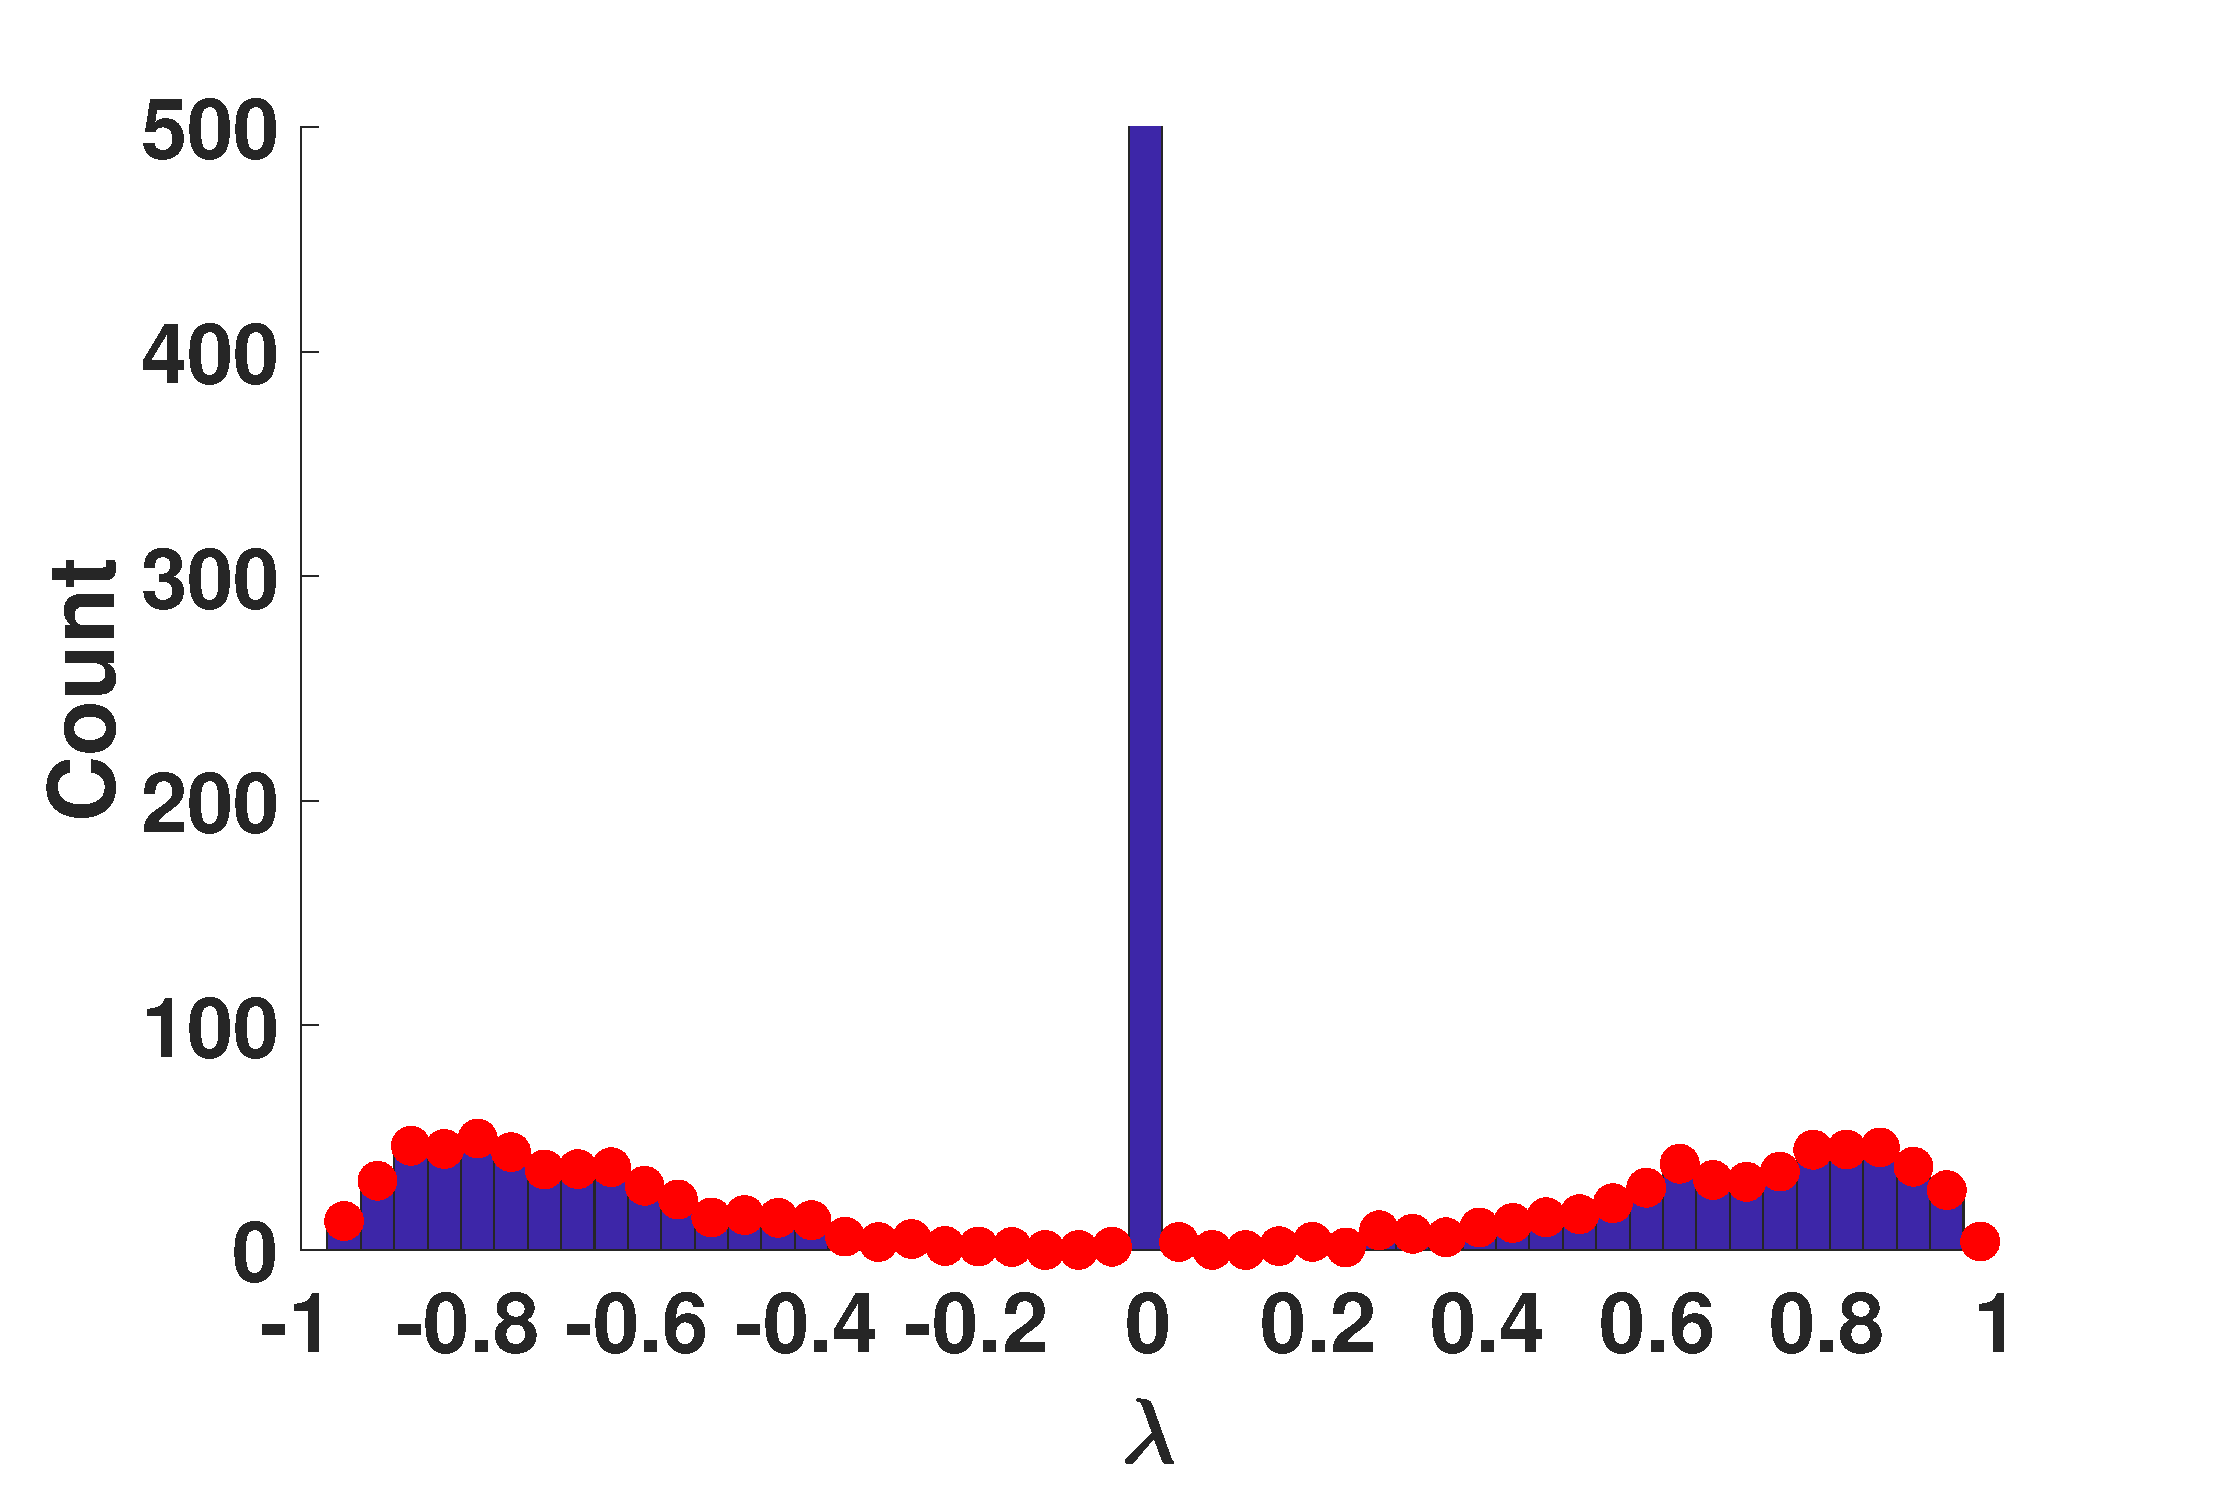
\includegraphics[width=\textwidth,trim = .4cm 0.5cm 3.5cm 1.3cm,clip]
    {./ndos/pics/erdos}
    \label{fig:erdos_dos}
  \end{subfigure}
  %
  \begin{subfigure}[t]{0.19\textwidth}
    \centering  
    \captionsetup{justification=centering,font=scriptsize}
    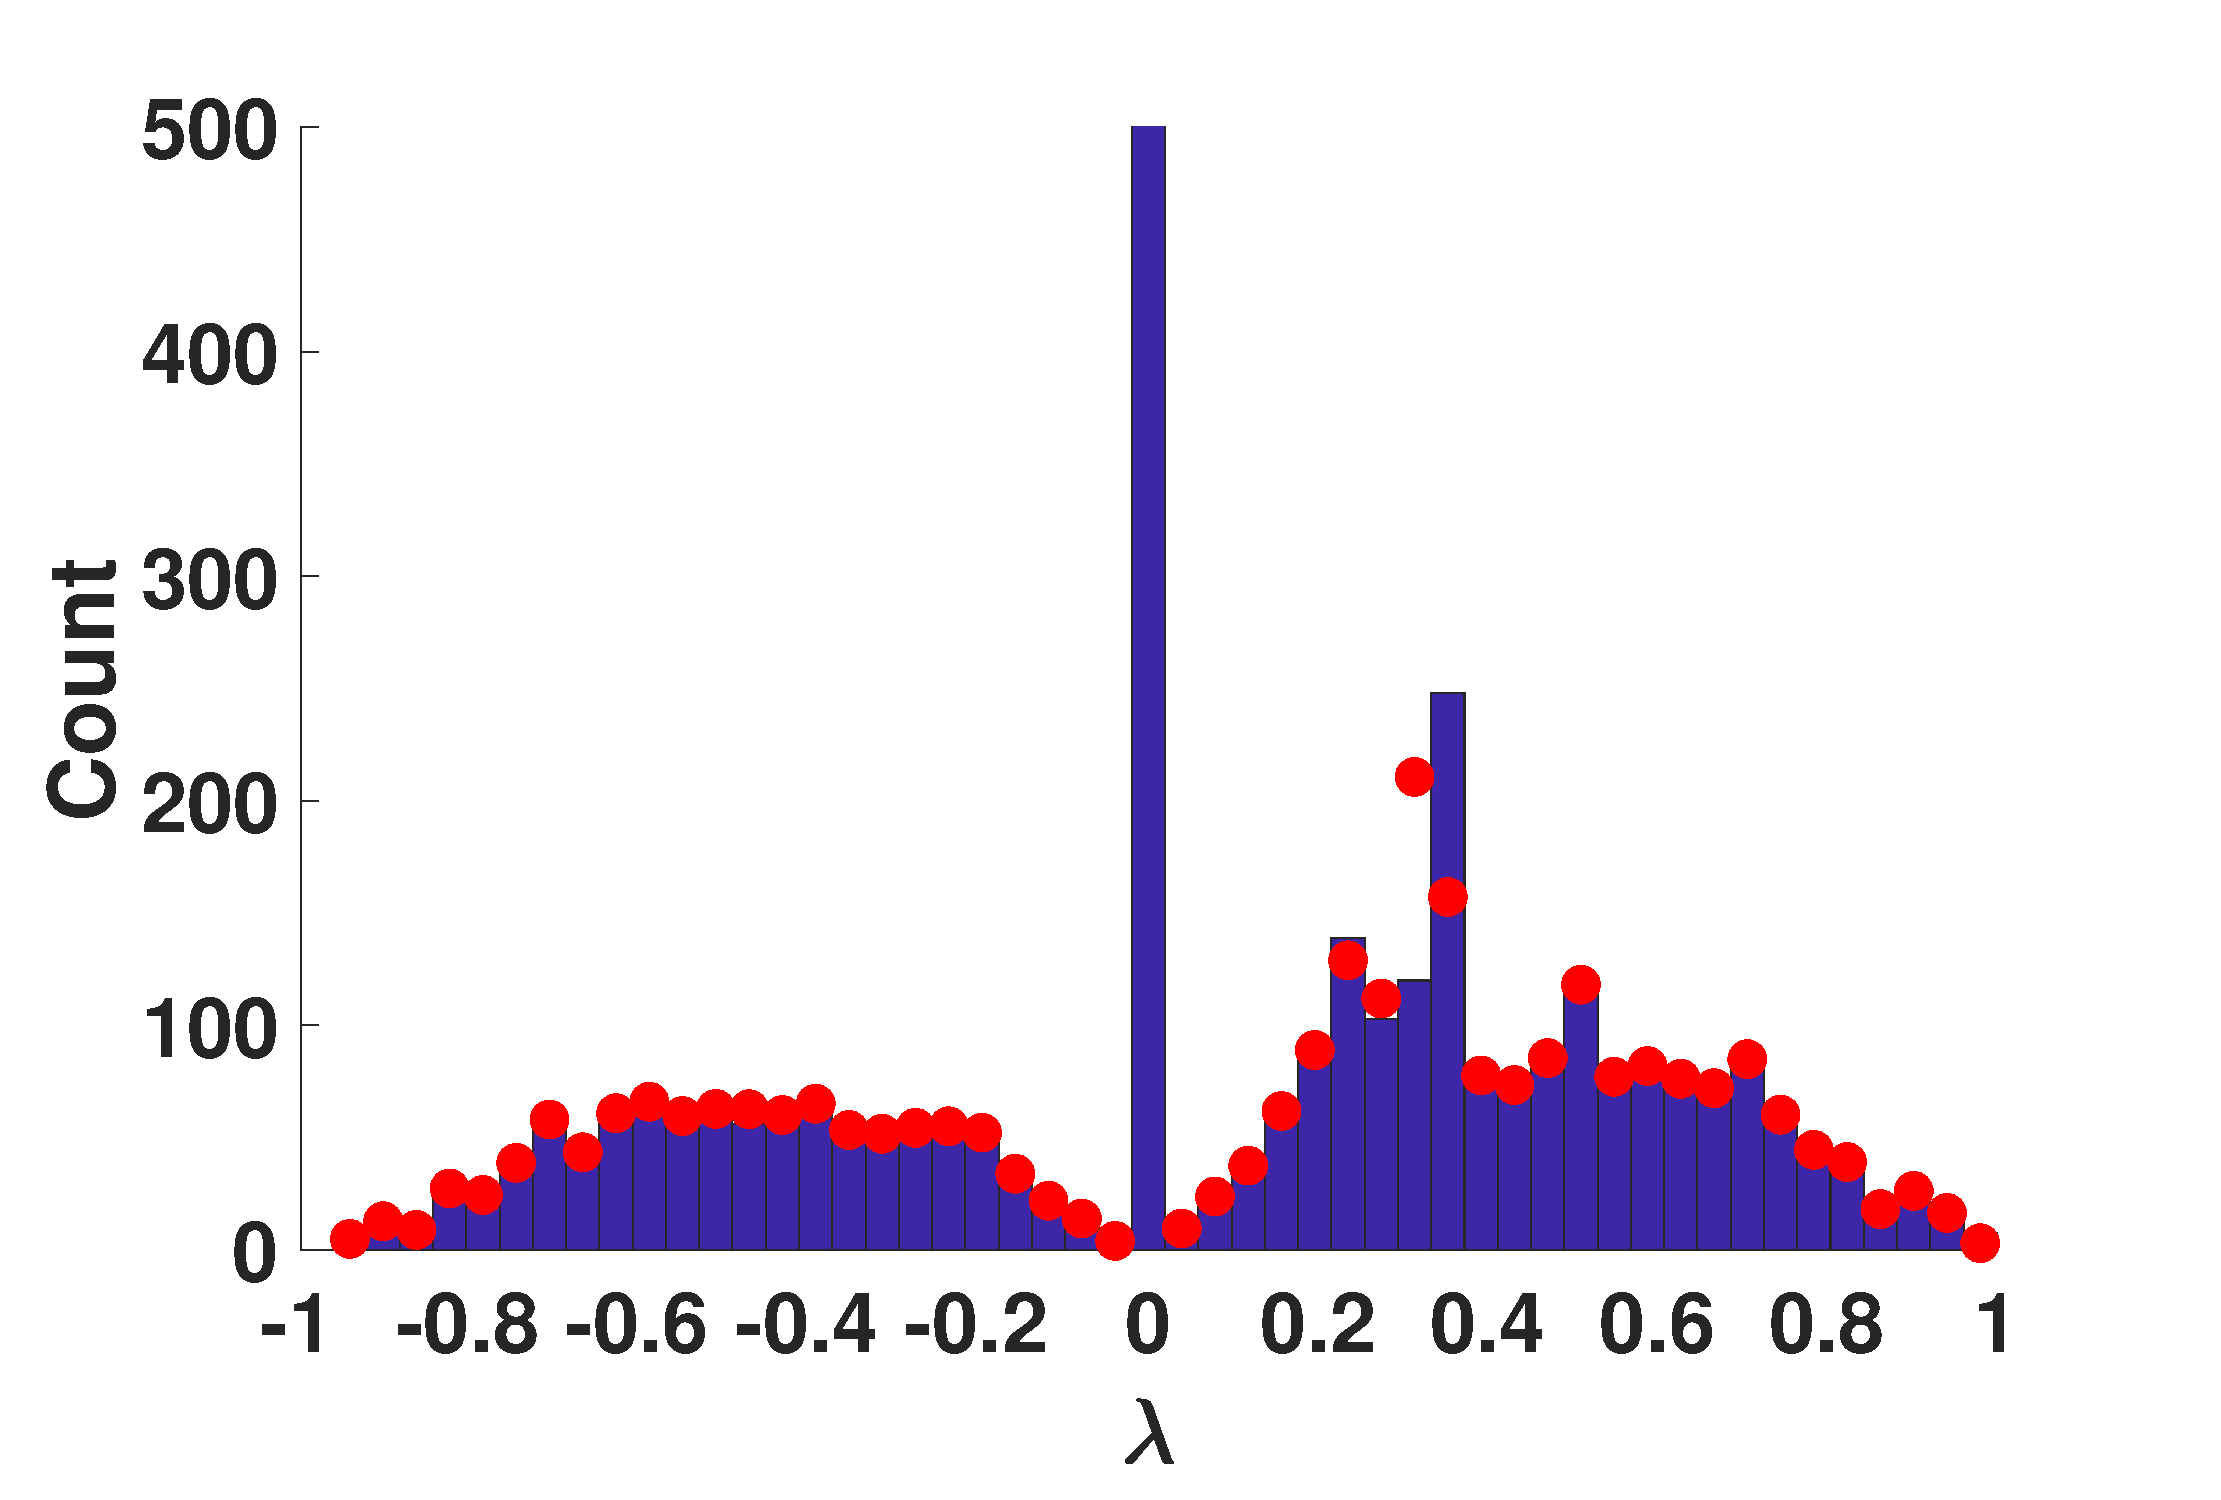
\includegraphics[width=\textwidth,trim = .4cm 0.5cm 3.5cm 1.3cm,clip]
    {./ndos/pics/as19991115}
    \label{fig:as_dos}
  \end{subfigure}
  %
  \begin{subfigure}[t]{0.19\textwidth}
    \centering
    \captionsetup{justification=centering,font=scriptsize}
    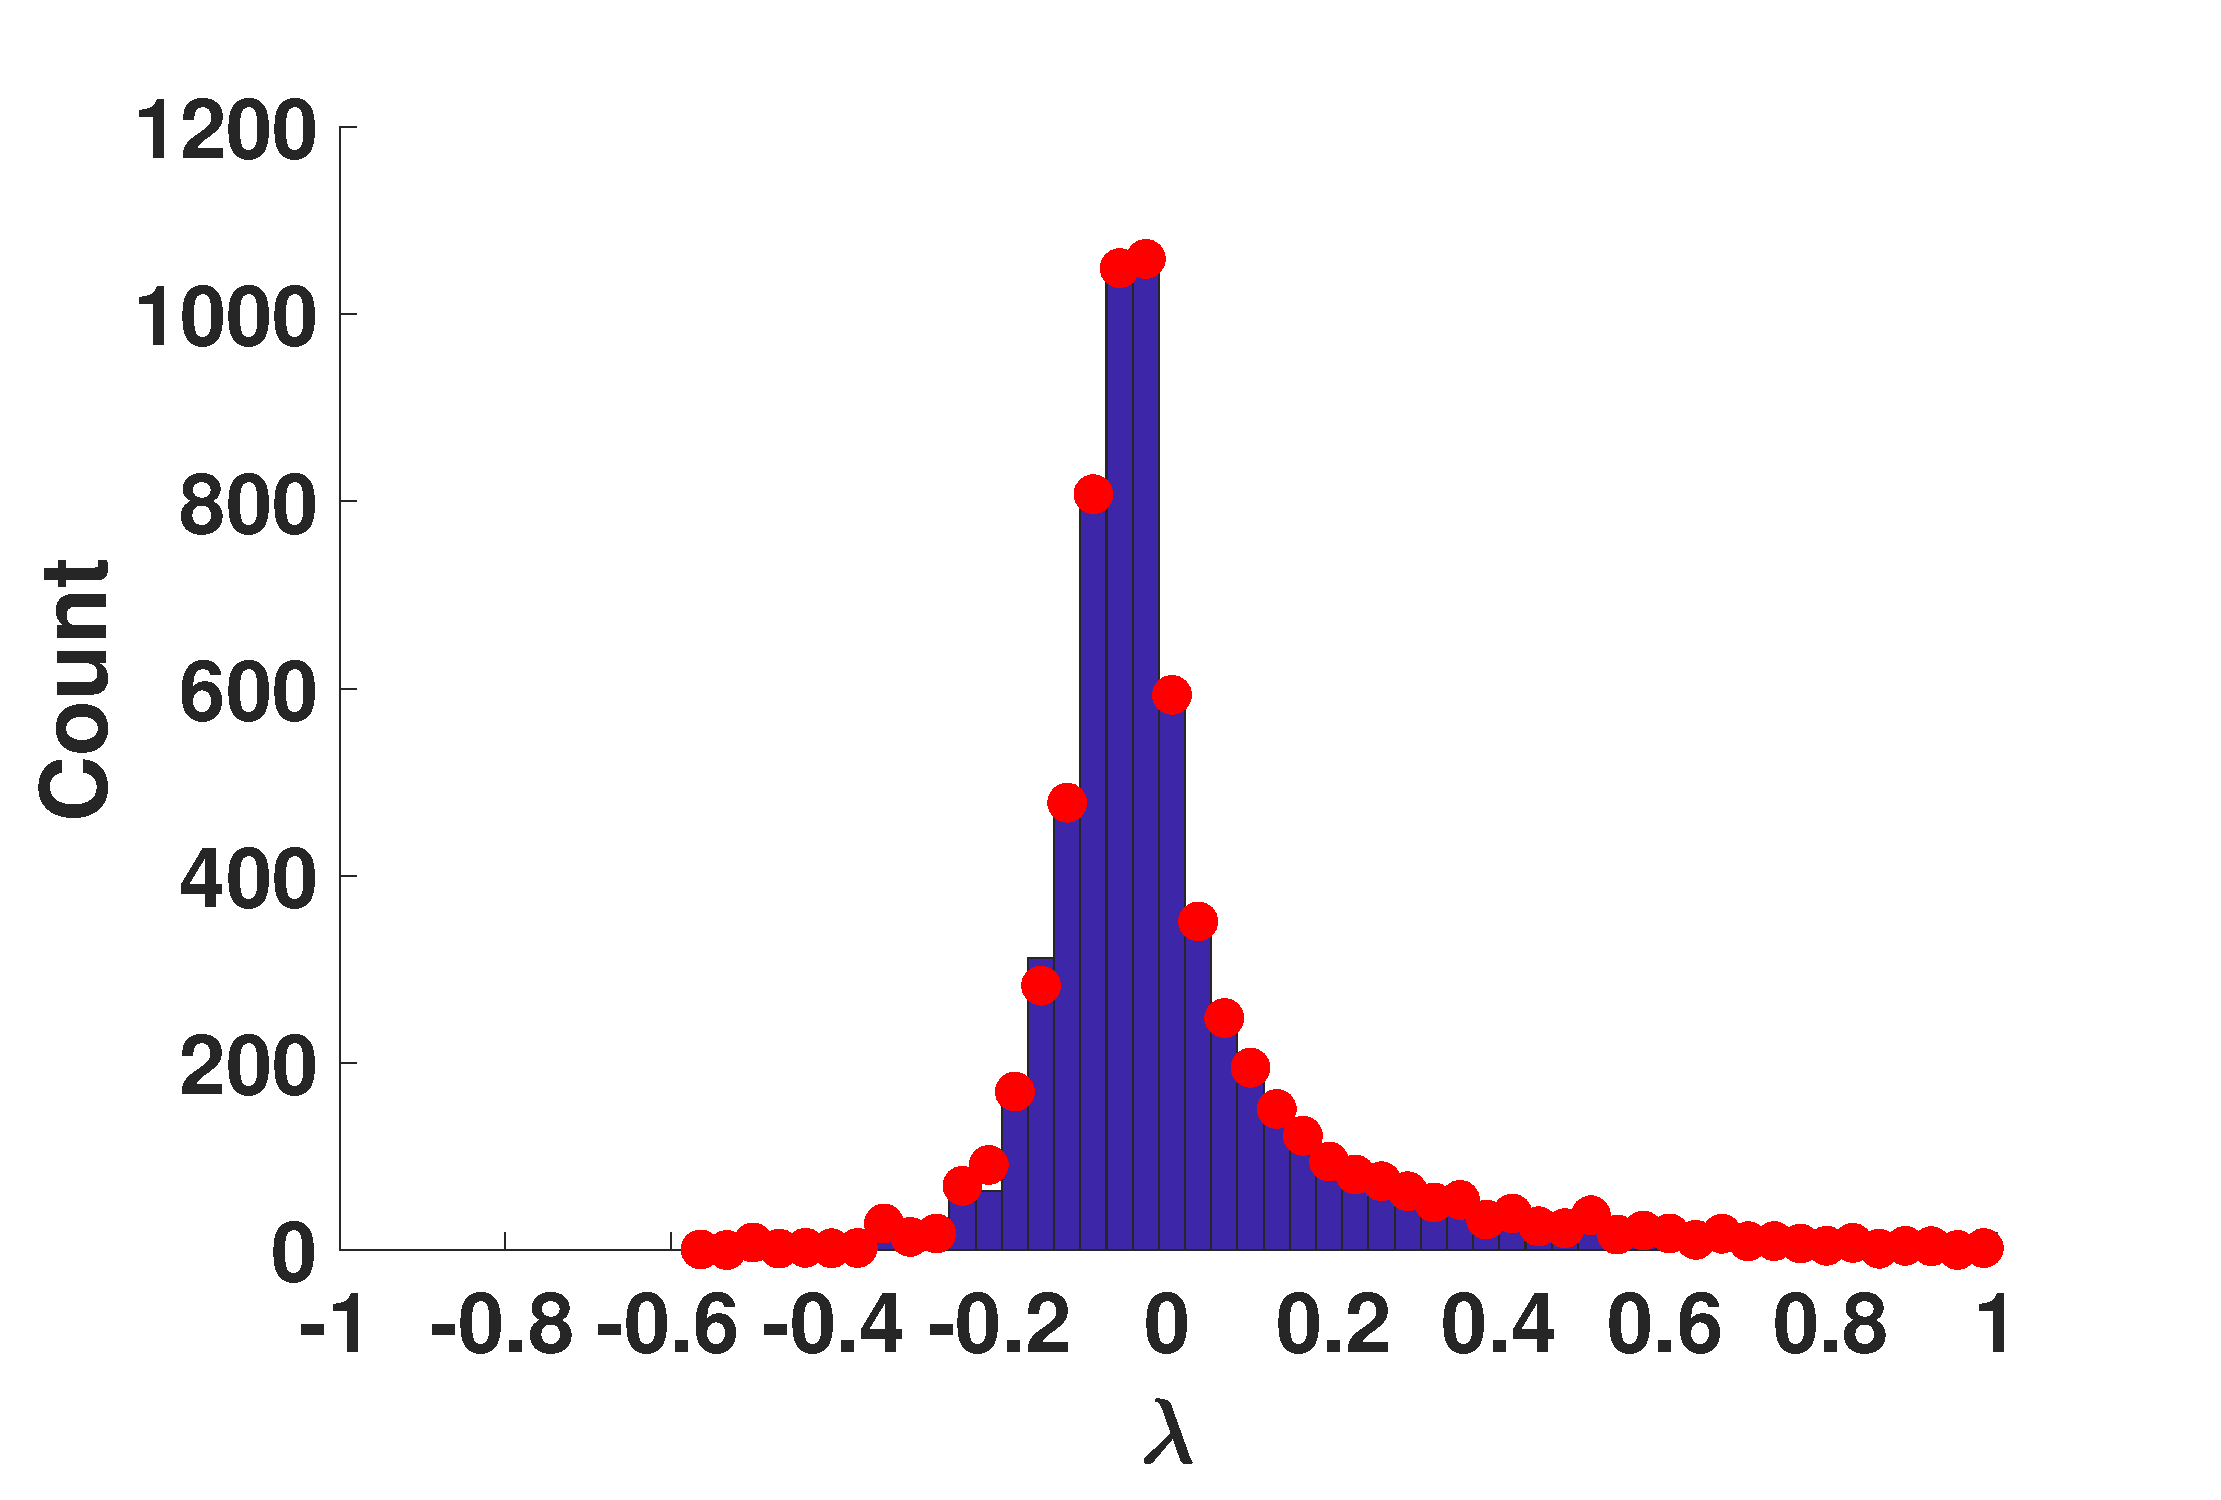
\includegraphics[width=\textwidth,trim = .4cm 0.5cm 3.5cm 1.3cm,clip]
    {./ndos/pics/marvel}
    \label{fig:marvel_dos}
  \end{subfigure}
  \begin{subfigure}[t]{0.19\textwidth}
    \centering  
    \captionsetup{justification=centering,font=scriptsize}
    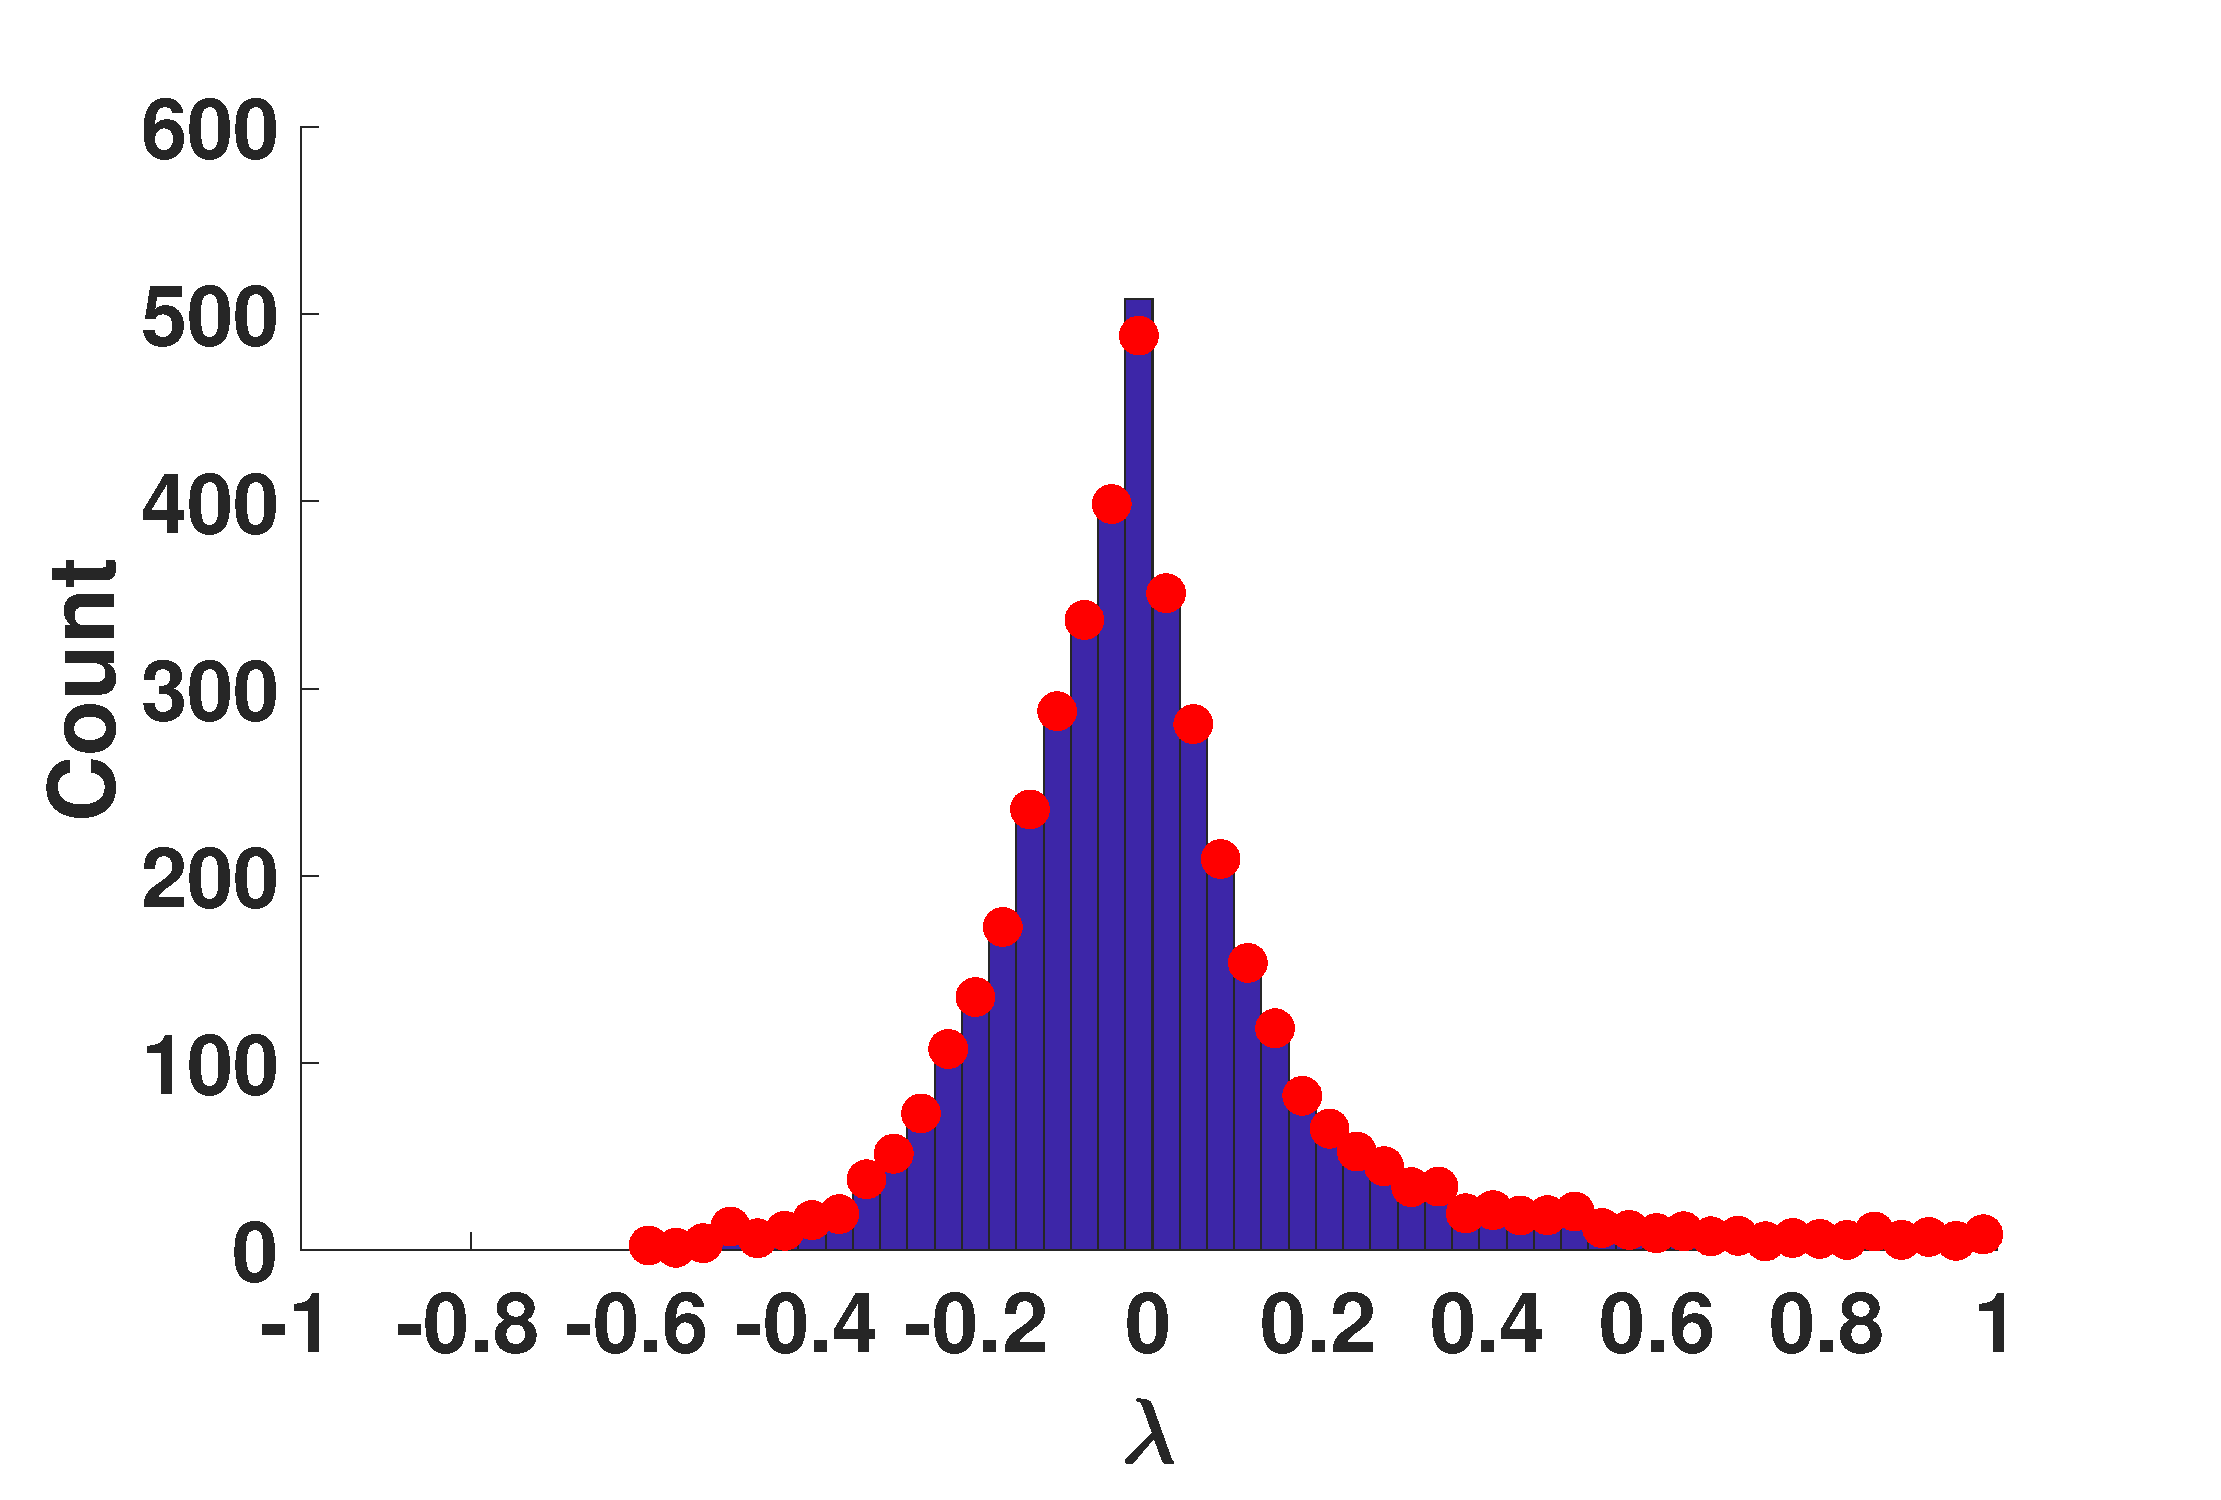
\includegraphics[width=\textwidth,trim = .4cm 0.5cm 3.5cm 1.3cm,clip]
    {./ndos/pics/facebook}
    \label{fig:facebook_dos}
  \end{subfigure}
  %
  \begin{subfigure}[t]{0.19\textwidth}
    \centering  
    \captionsetup{justification=centering,font=scriptsize}
    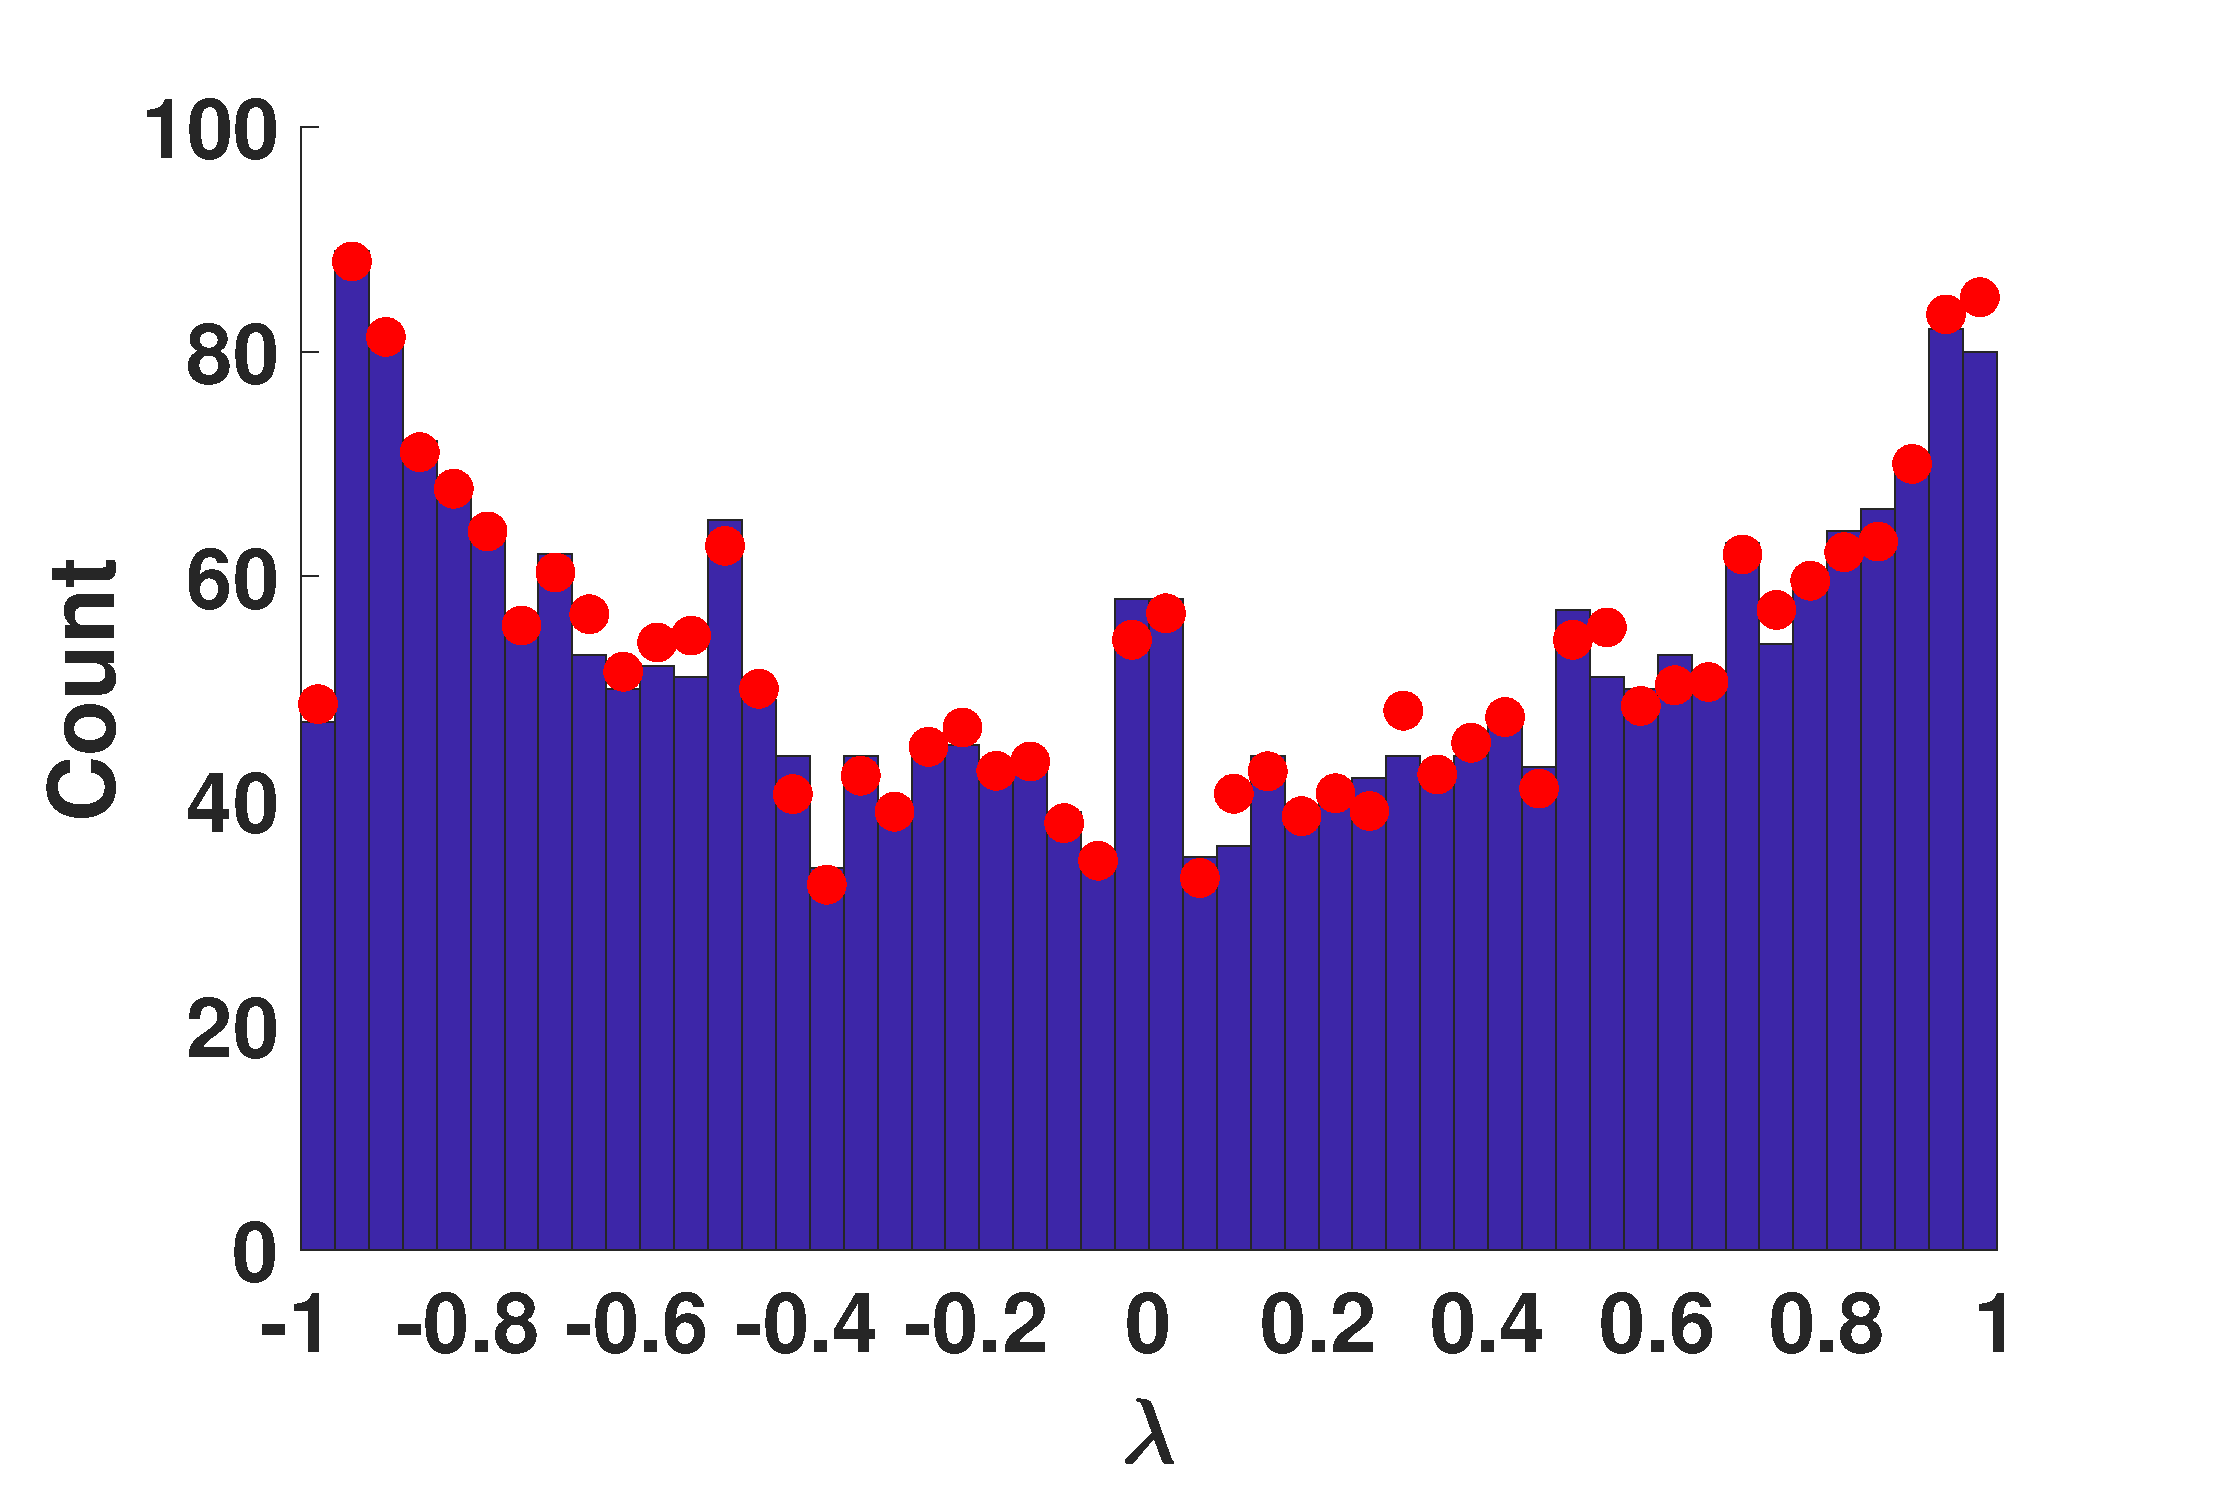
\includegraphics[width=\textwidth,trim = .4cm 0.5cm 3.5cm 1.3cm,clip]
    {./ndos/pics/minnesota}
    \label{fig:minnesota_dos}
  \end{subfigure}
  %
  \begin{subfigure}[t]{0.19\textwidth}
    \centering  
    \captionsetup{justification=centering,font=scriptsize}
    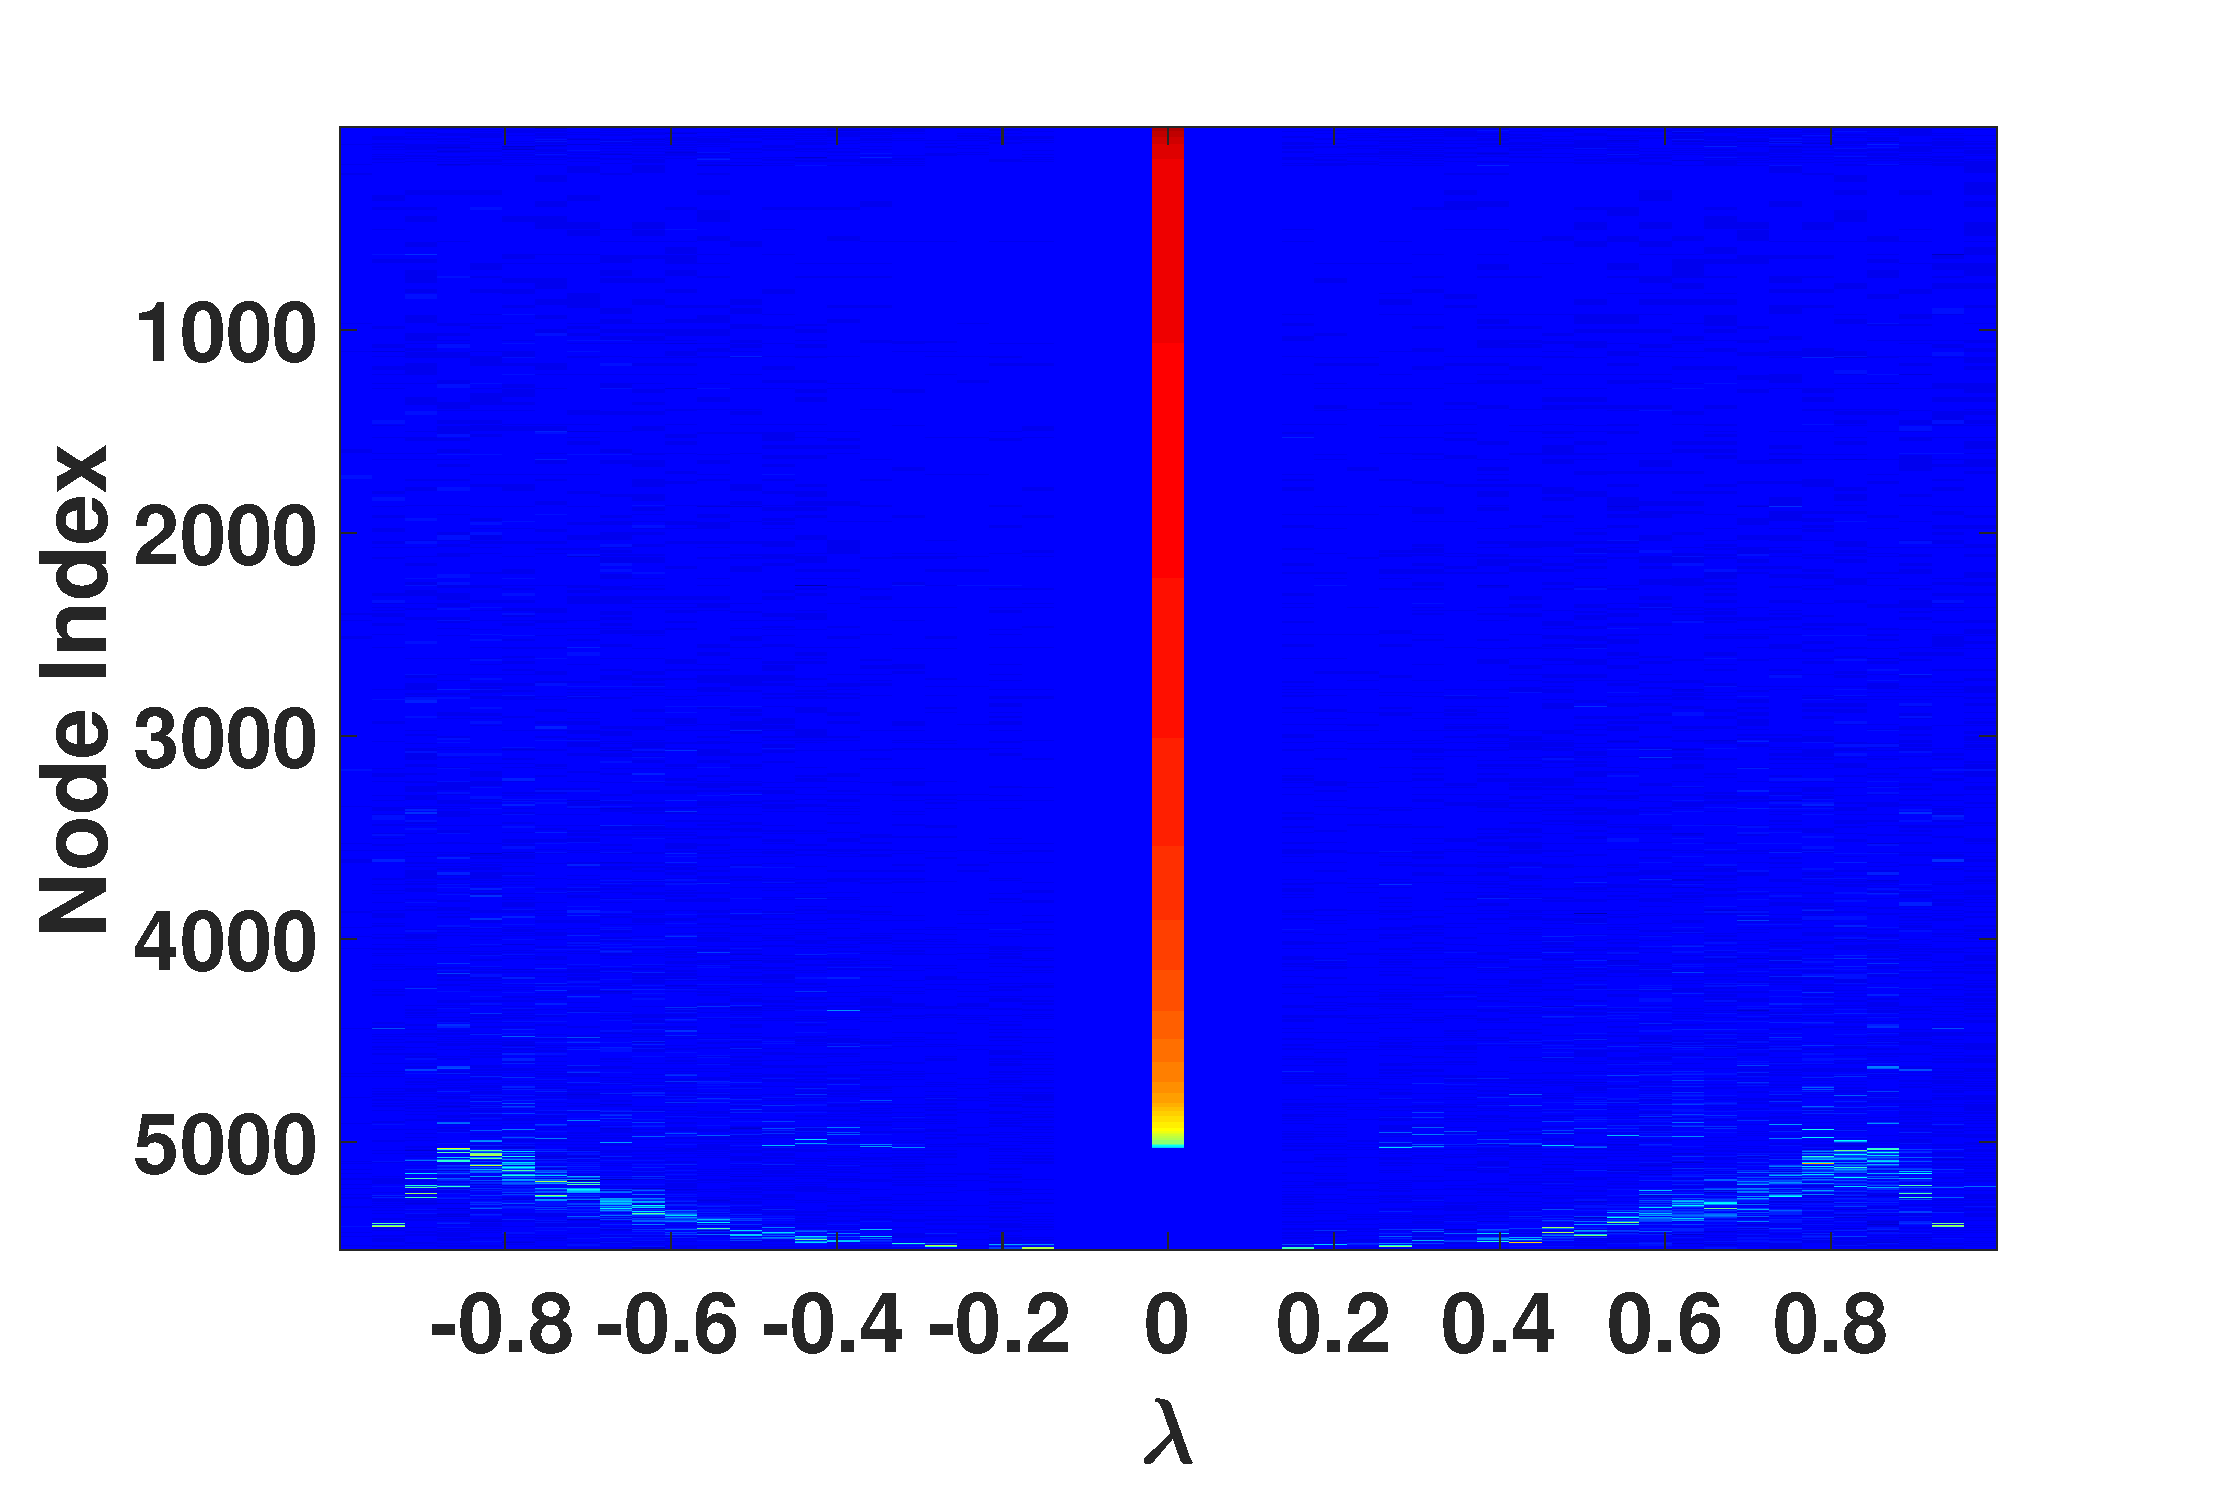
\includegraphics[width=\textwidth,trim = .4cm 0.5cm 3.5cm 1.3cm,clip]
    {./ndos/pics/erdos_ldos}
    \caption{Erd\H{o}s Collaboration Network}
    \label{fig:erdos_ldos}
  \end{subfigure}
  %
  \begin{subfigure}[t]{0.19\textwidth}
    \centering  
    \captionsetup{justification=centering,font=scriptsize}
    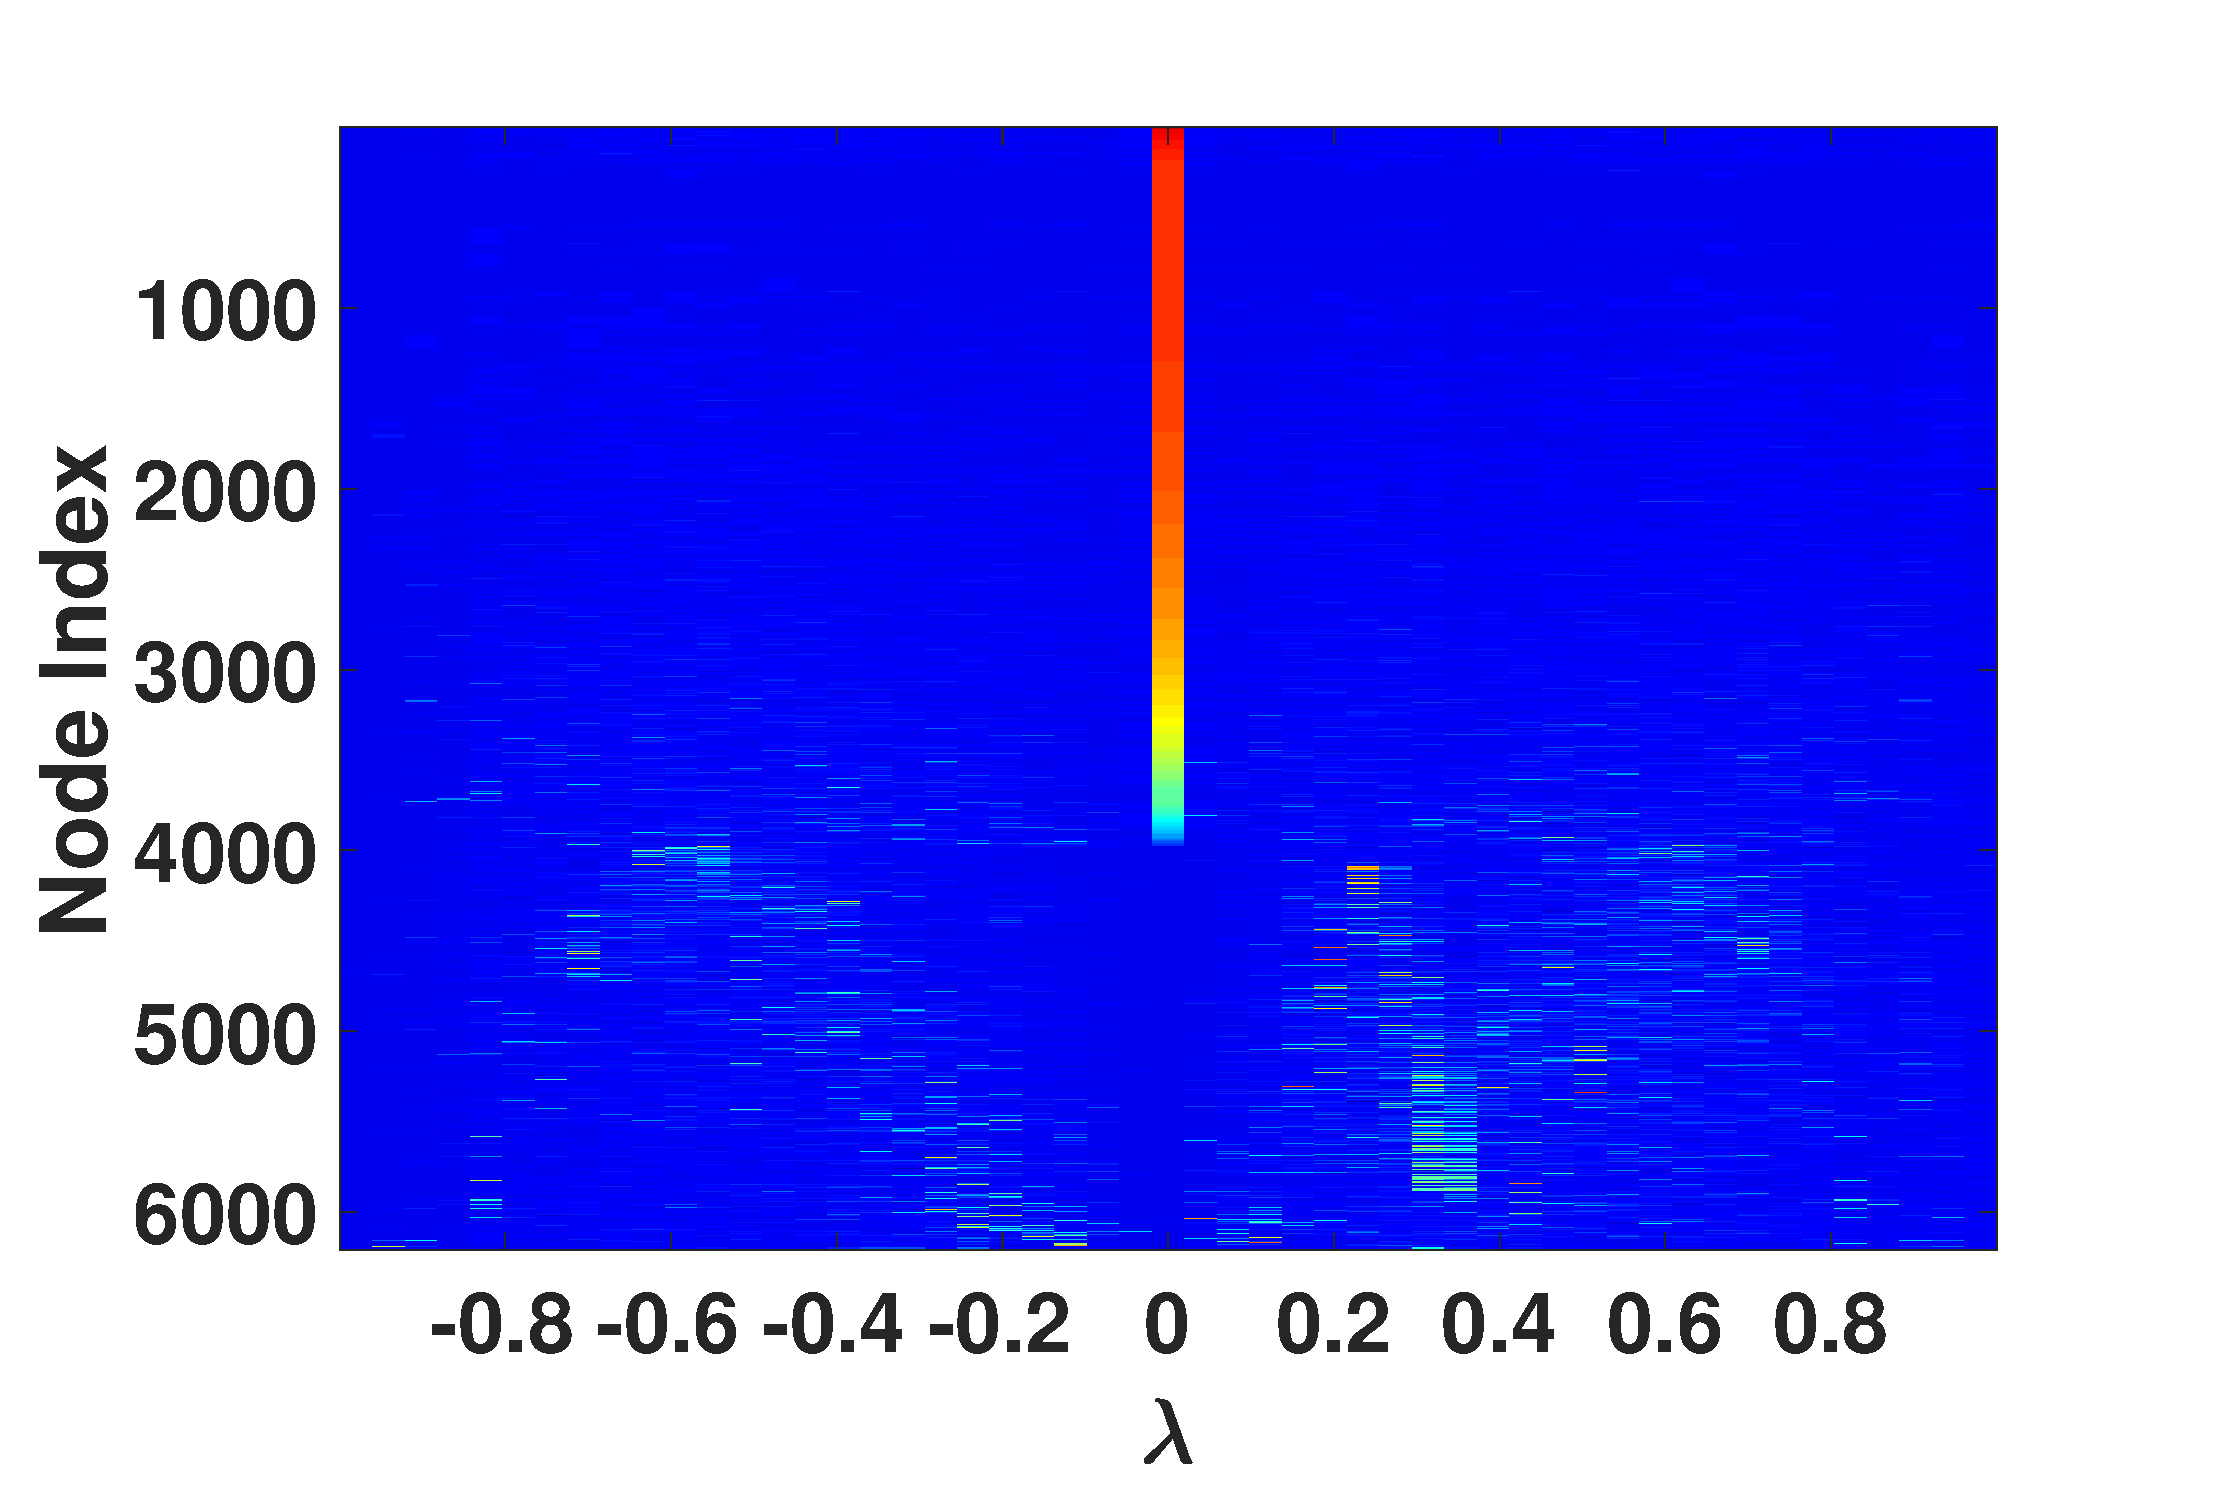
\includegraphics[width=\textwidth,trim = .4cm 0.5cm 3.5cm 1.3cm,clip]
    {./ndos/pics/as19991115_ldos}
    \caption{Autonomous System Network (1999)}
    \label{fig:as_ldos}
  \end{subfigure}
  %
  \begin{subfigure}[t]{0.19\textwidth}
    \centering  
    \captionsetup{justification=centering,font=scriptsize}
    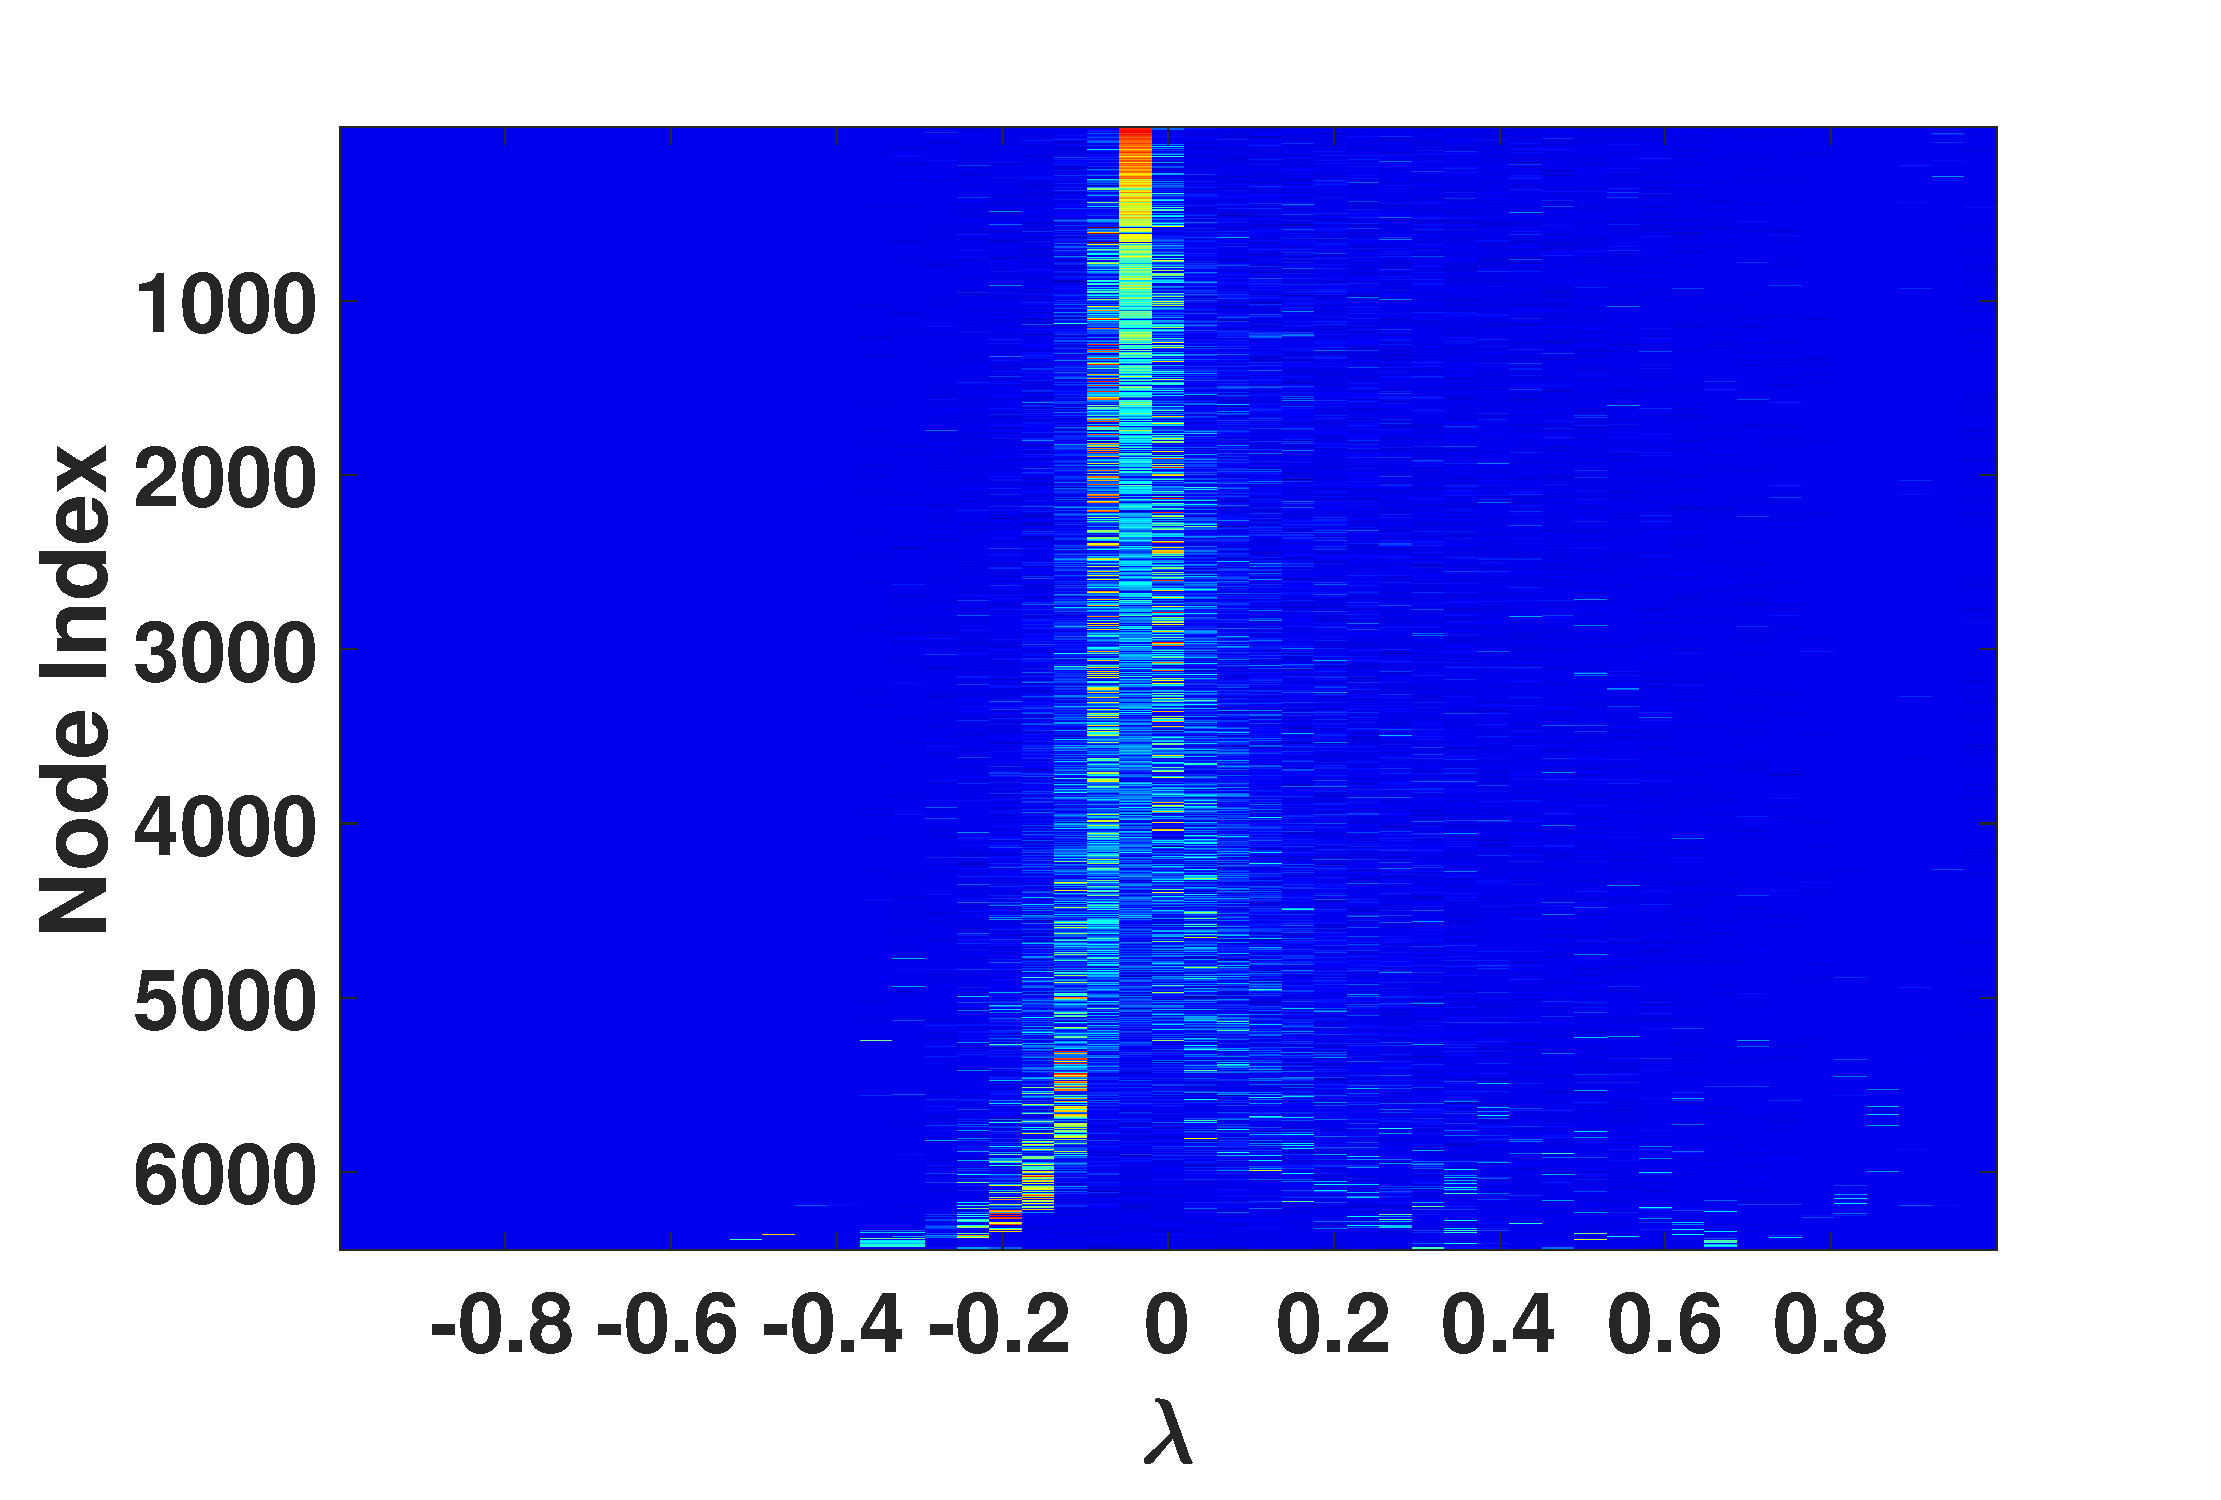
\includegraphics[width=\textwidth,trim = .4cm 0.5cm 3.5cm 1.3cm,clip]
    {./ndos/pics/marvel_ldos}{}
    \caption{Marvel Characters Network}
    \label{fig:marvel_ldos}
  \end{subfigure}
  %
  \begin{subfigure}[t]{0.19\textwidth}
    \centering  
    \captionsetup{justification=centering,font=scriptsize}
    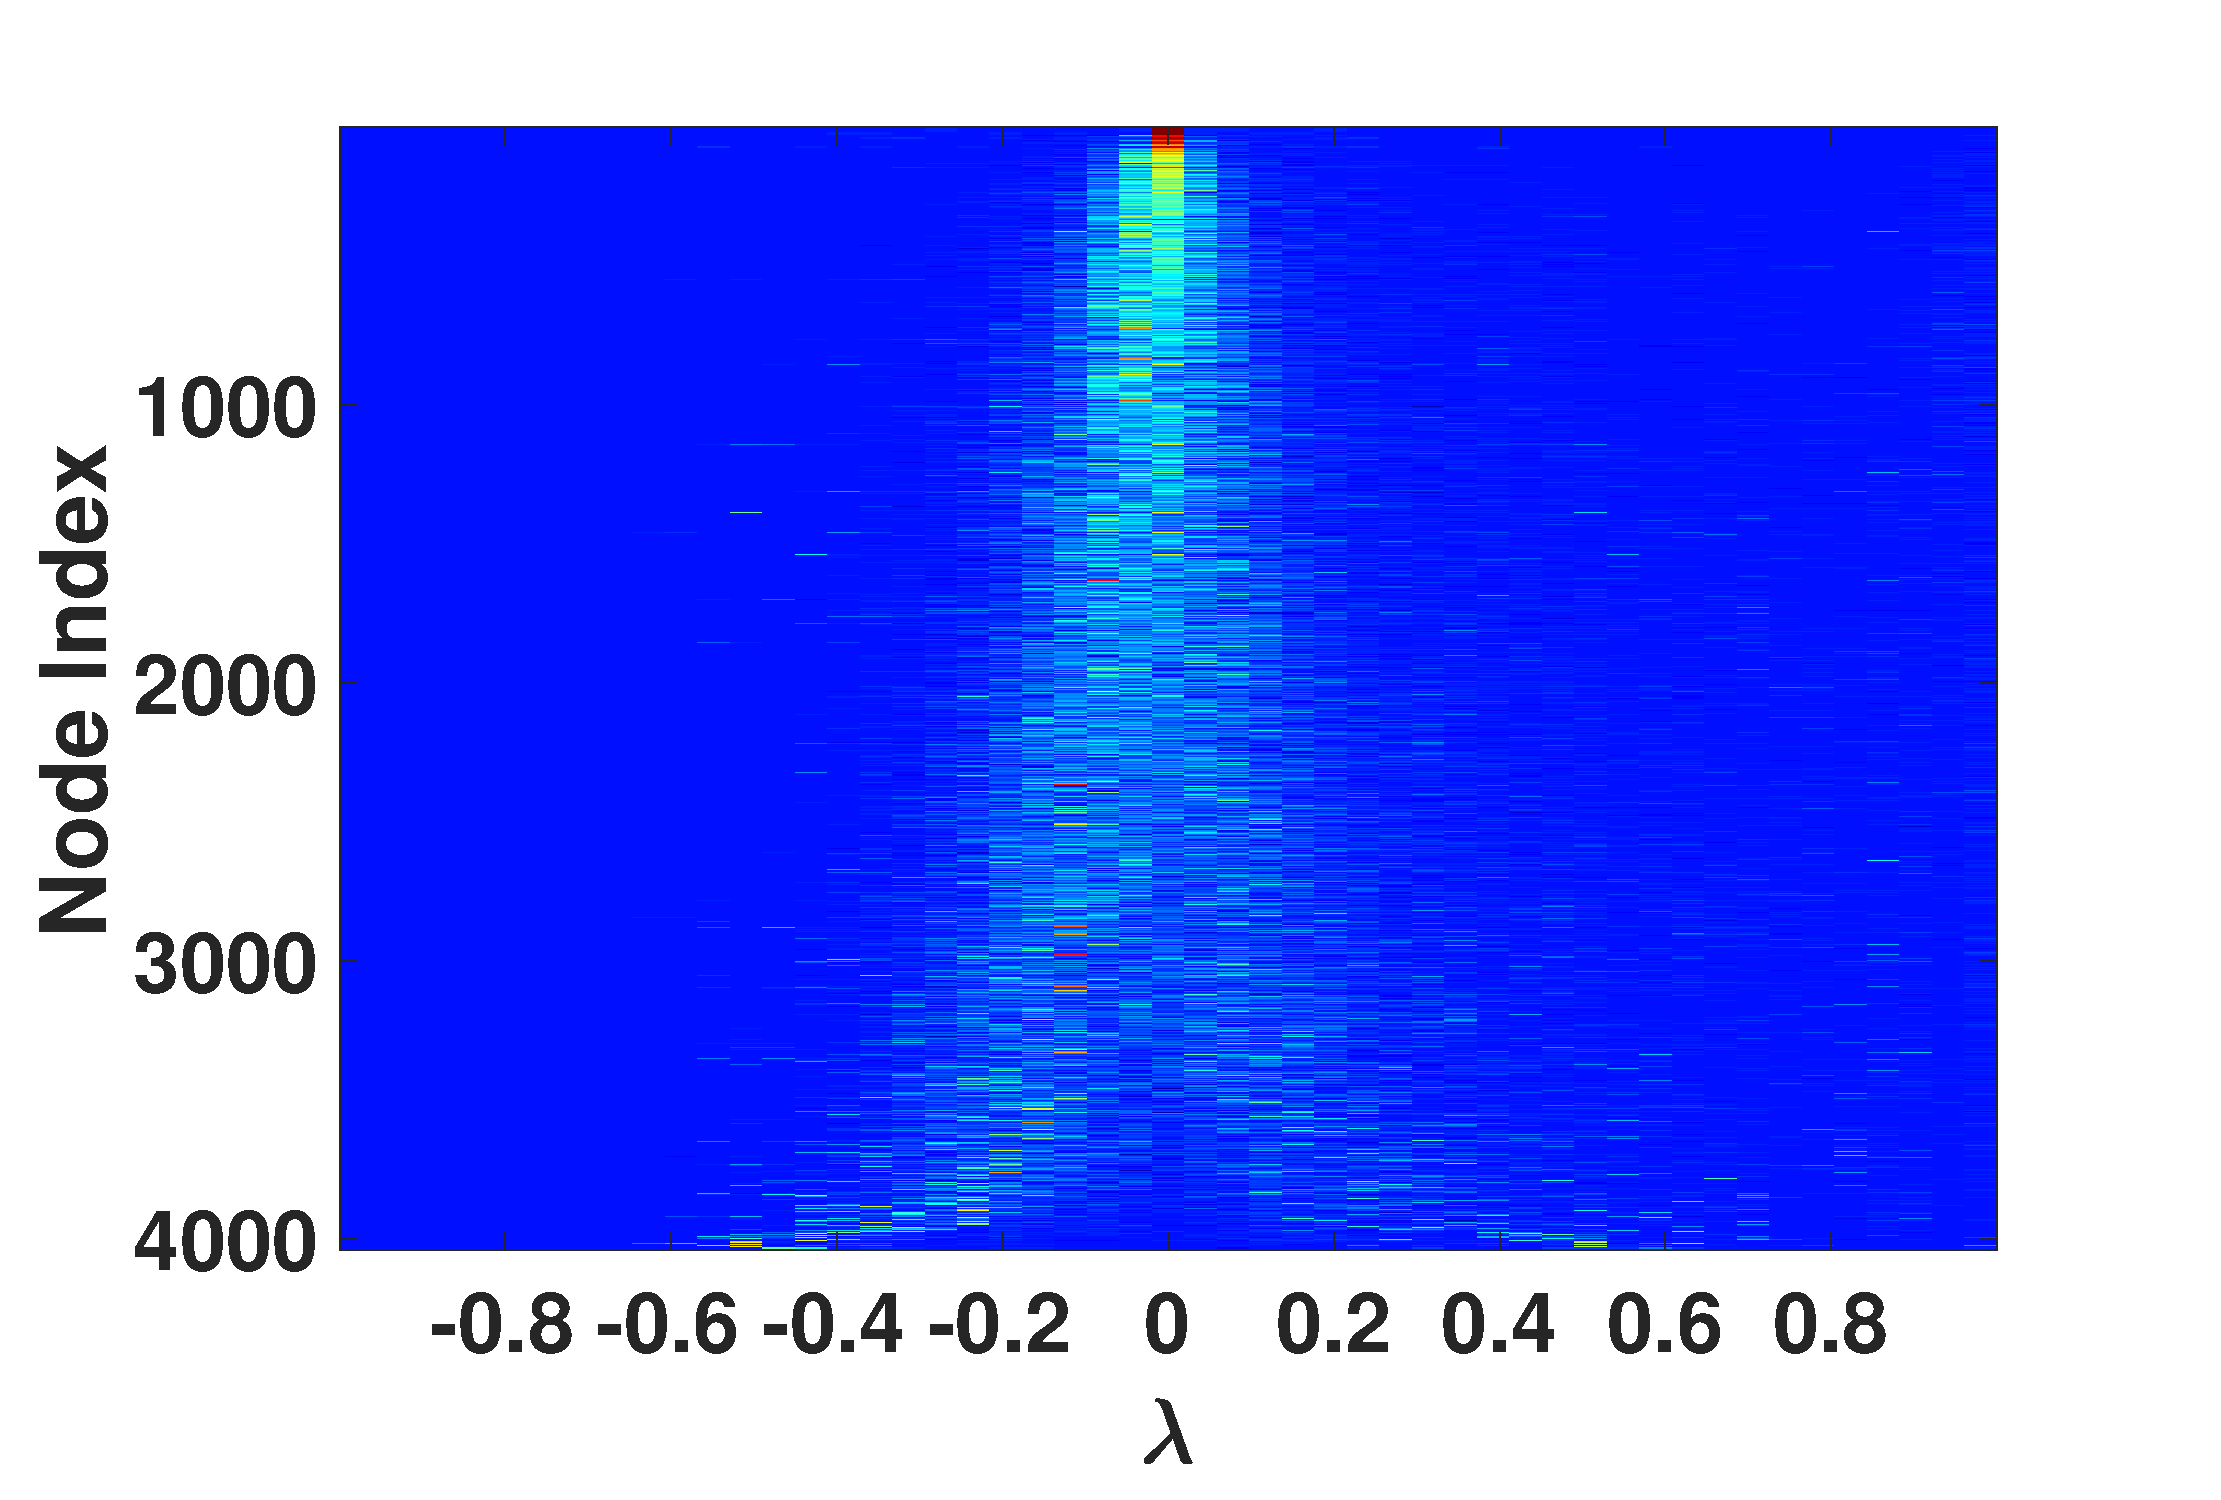
\includegraphics[width=\textwidth,trim = .4cm 0.5cm 3.5cm 1.3cm,clip]
    {./ndos/pics/facebook_ldos}
    \caption{Facebook Ego Networks}
    \label{fig:facebook_ldos}
  \end{subfigure}
  %
  \begin{subfigure}[t]{0.19\textwidth}
    \centering  
    \captionsetup{justification=centering,font=scriptsize}
    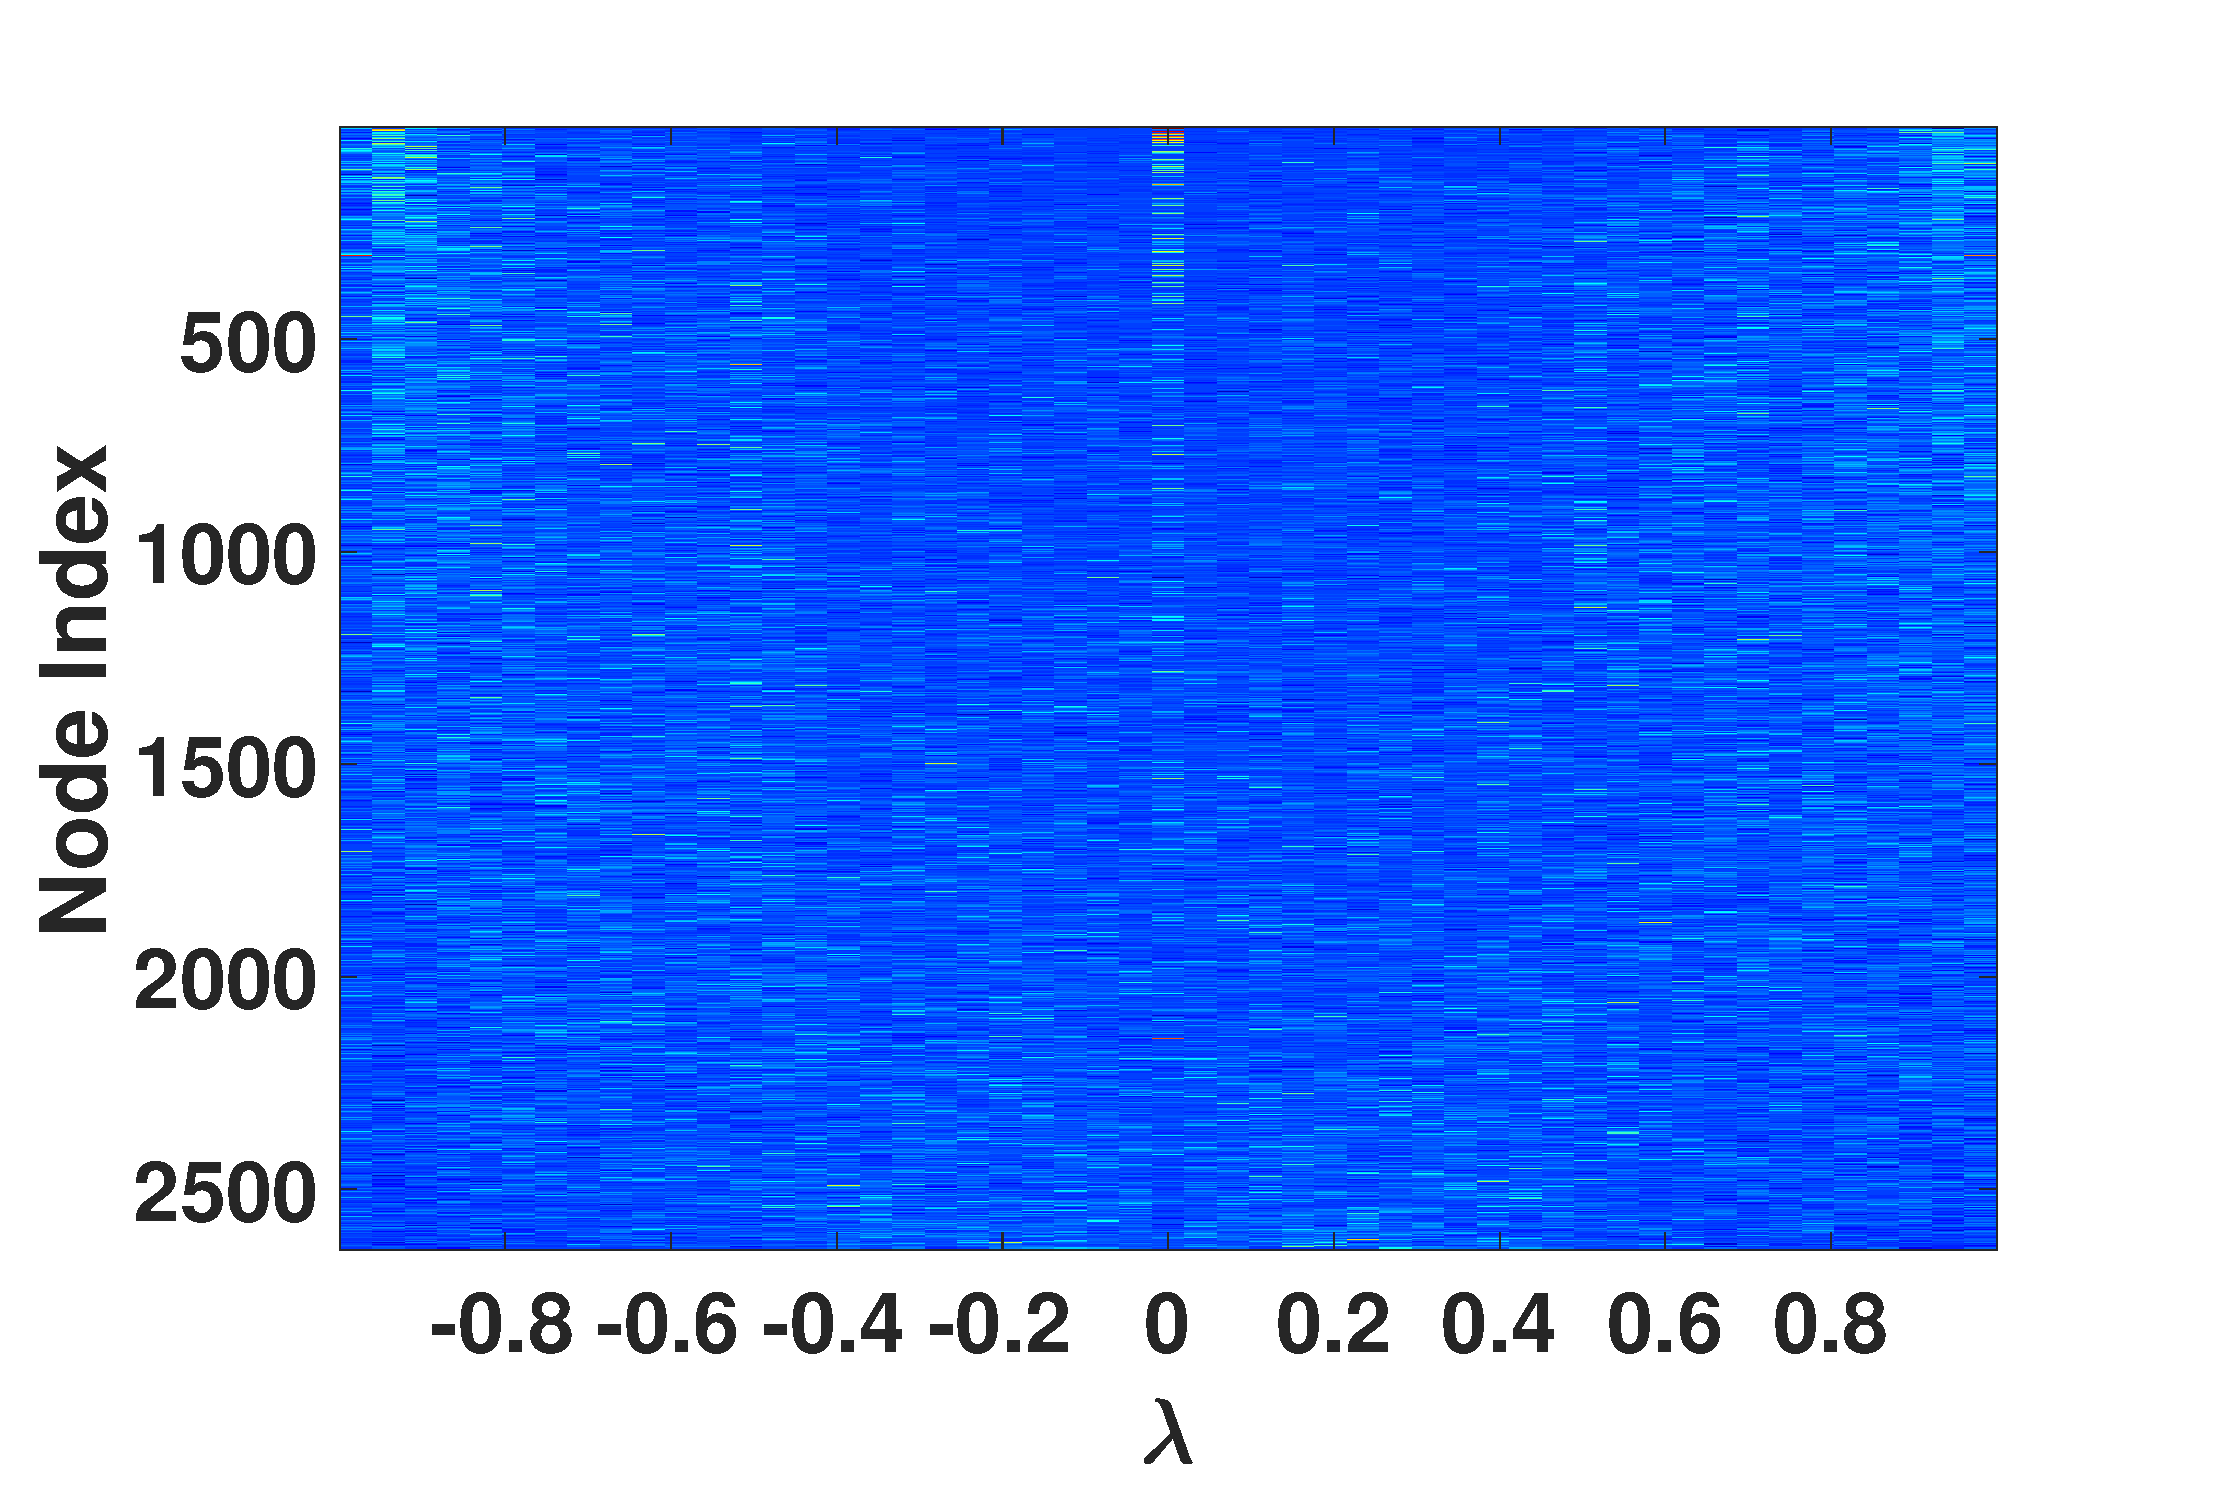
\includegraphics[width=\textwidth,trim = .4cm 0.5cm 3.5cm 1.3cm,clip]
    {./ndos/pics/minnesota_ldos}
    \caption{Minnesota Road Network}
    \label{fig:minnesota_ldos}
  \end{subfigure}
  %
  \begin{subfigure}[t]{0.19\textwidth}
    \centering  
    \captionsetup{justification=centering,font=scriptsize}
    \includegraphics[width=\textwidth,trim = .4cm 0.5cm 3.5cm 1.3cm,clip]
    {./ndos/pics/hepth}
    \label{fig:hepth_dos}
  \end{subfigure}
  %
  \begin{subfigure}[t]{0.19\textwidth}
    \centering  
    \captionsetup{justification=centering,font=scriptsize}
    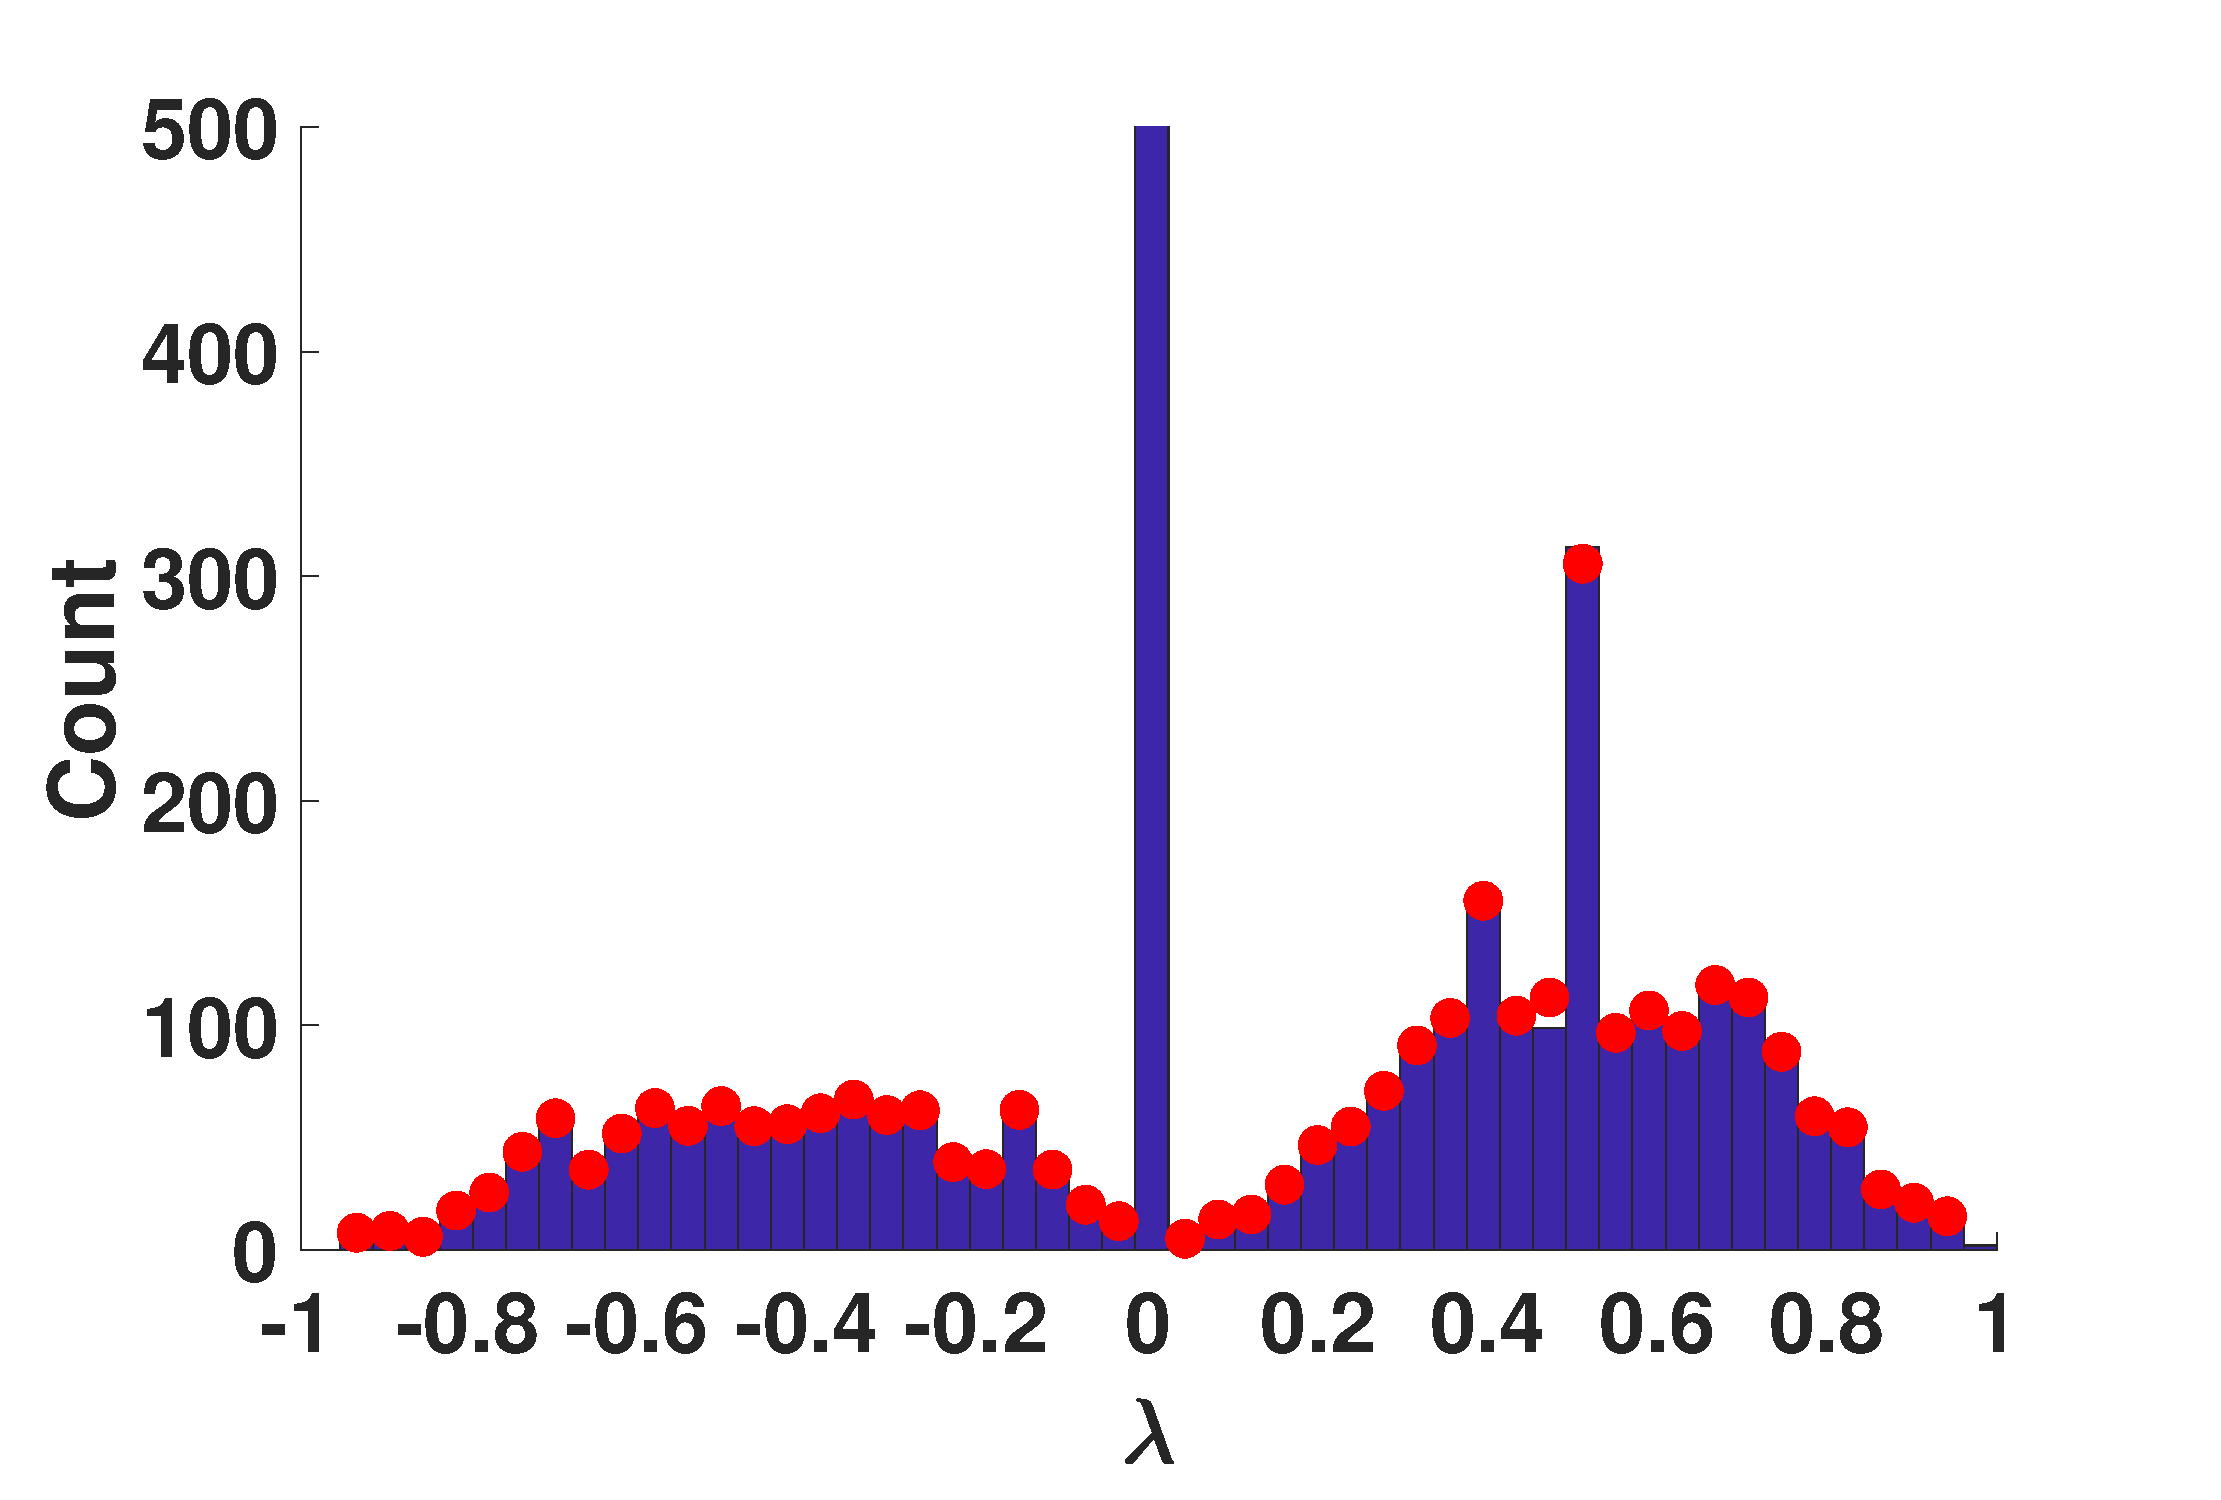
\includegraphics[width=\textwidth,trim = .4cm 0.5cm 3.5cm 1.3cm,clip]
    {./ndos/pics/as20000102}
    \label{fig:as2_dos}
  \end{subfigure}
  %
  \begin{subfigure}[t]{0.19\textwidth}
    \centering
    \captionsetup{justification=centering,font=scriptsize}
    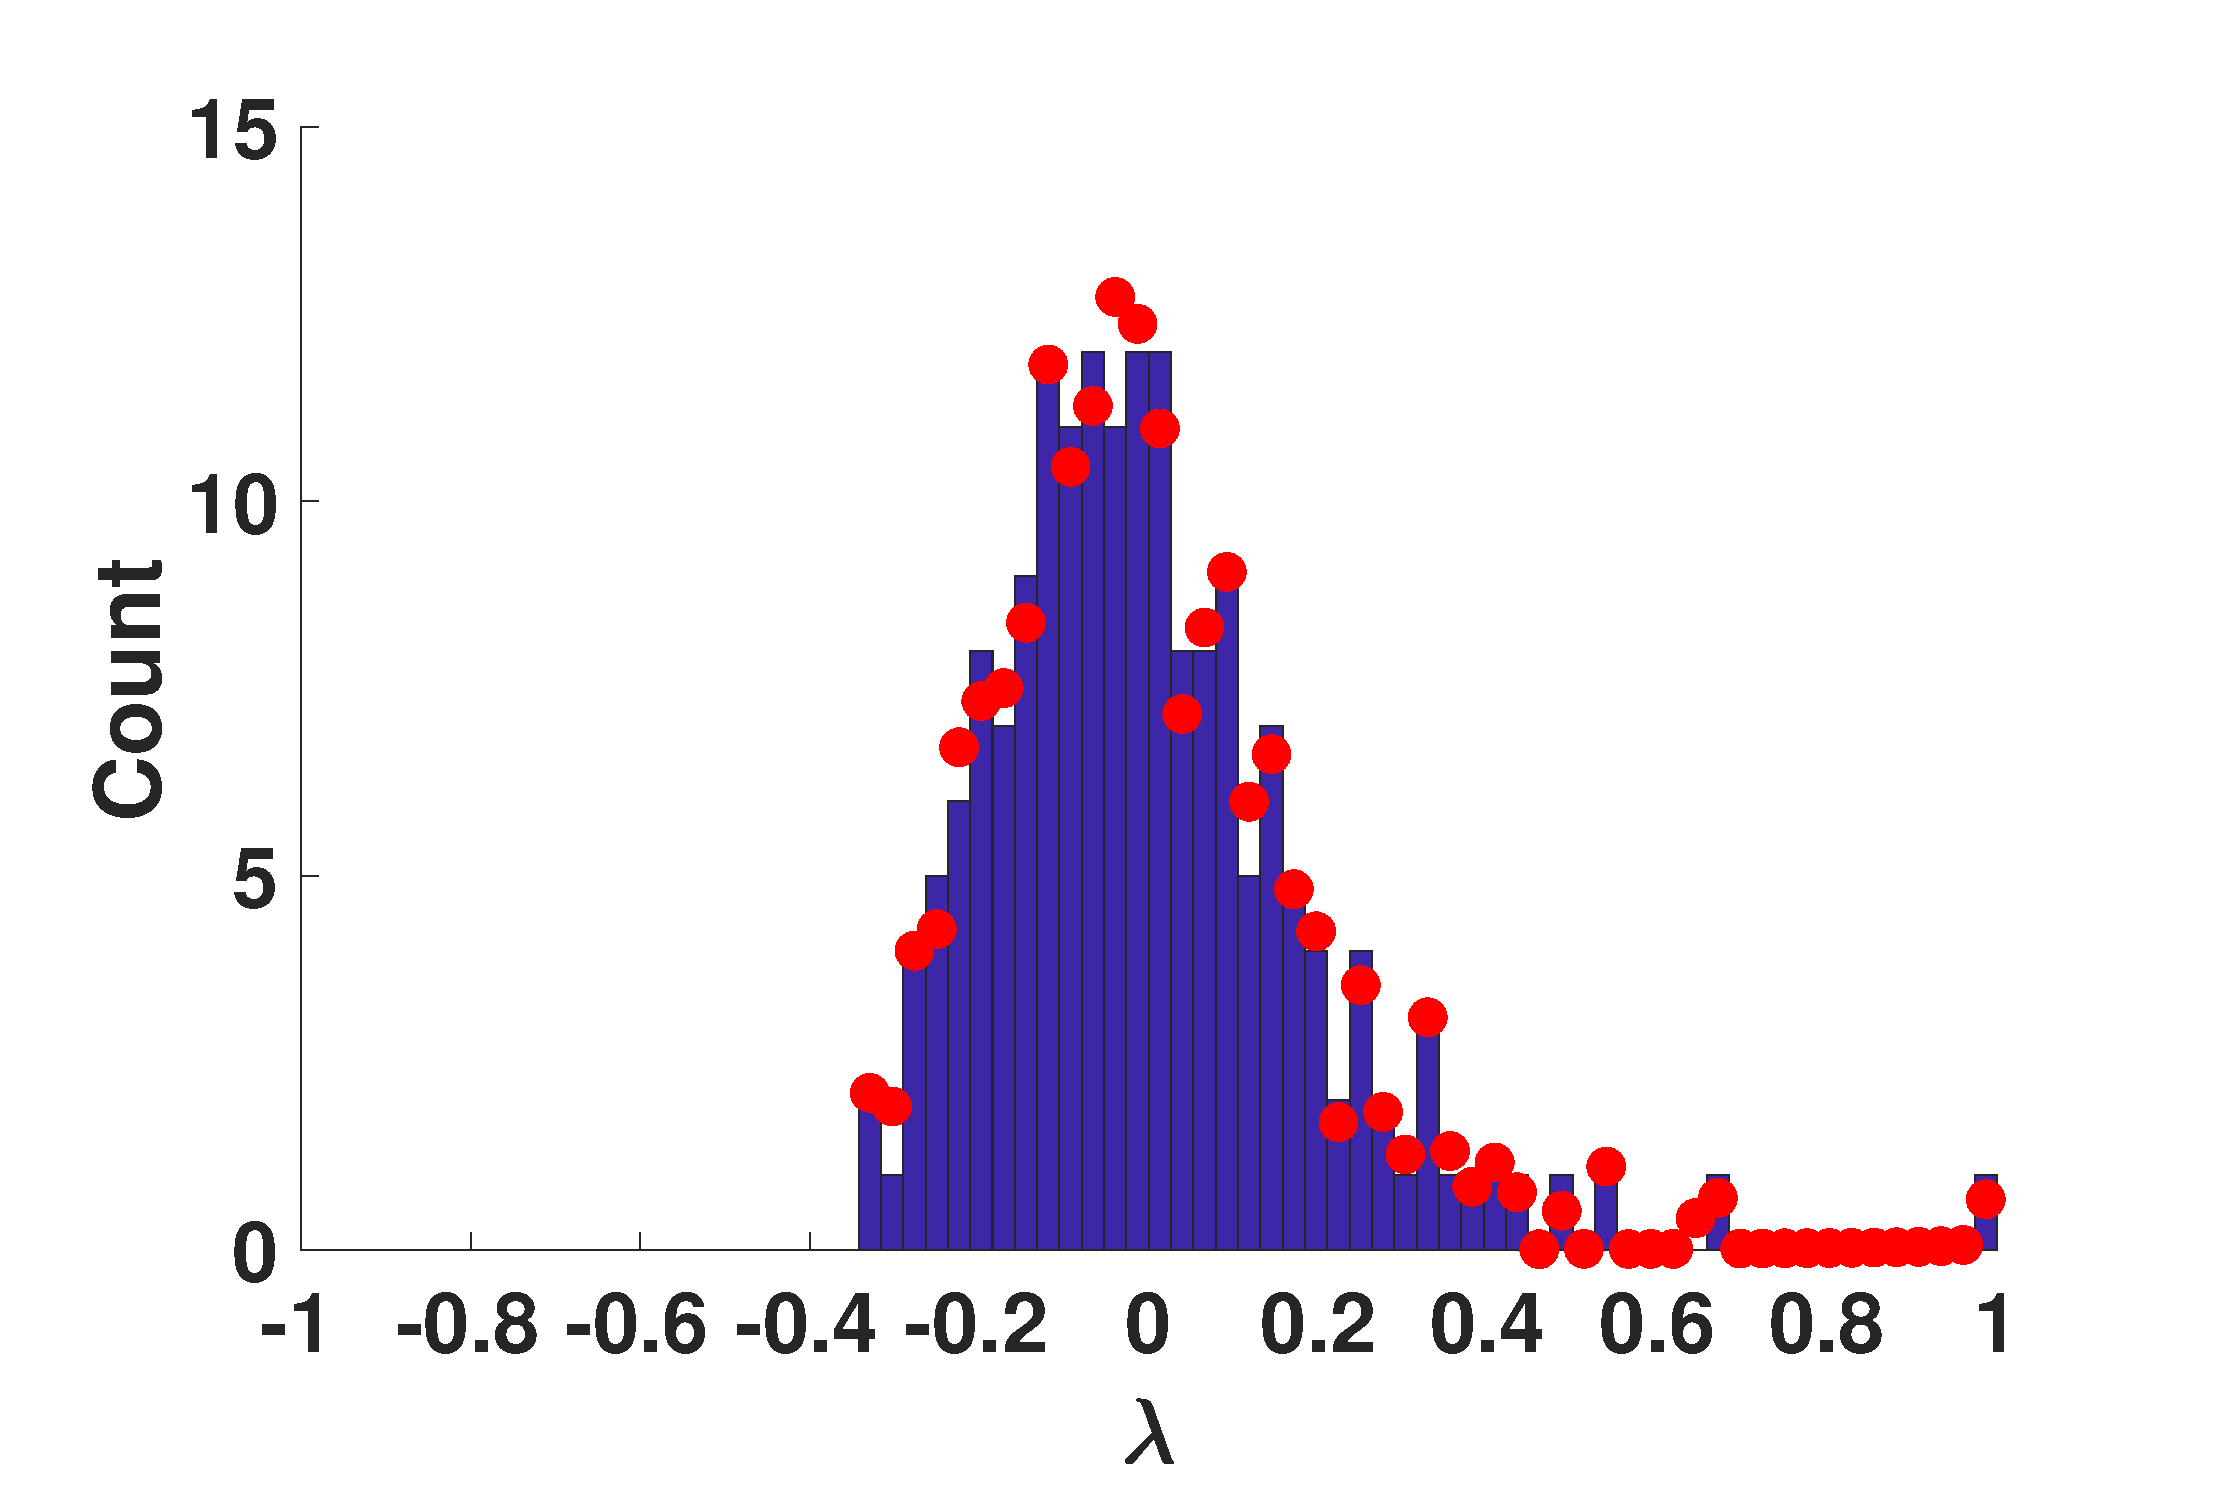
\includegraphics[width=\textwidth,trim = .4cm 0.5cm 3.5cm 1.3cm,clip]
    {./ndos/pics/hp}
    \label{fig:hp_dos}
  \end{subfigure}
  \begin{subfigure}[t]{0.19\textwidth}
    \centering  
    \captionsetup{justification=centering,font=scriptsize}
    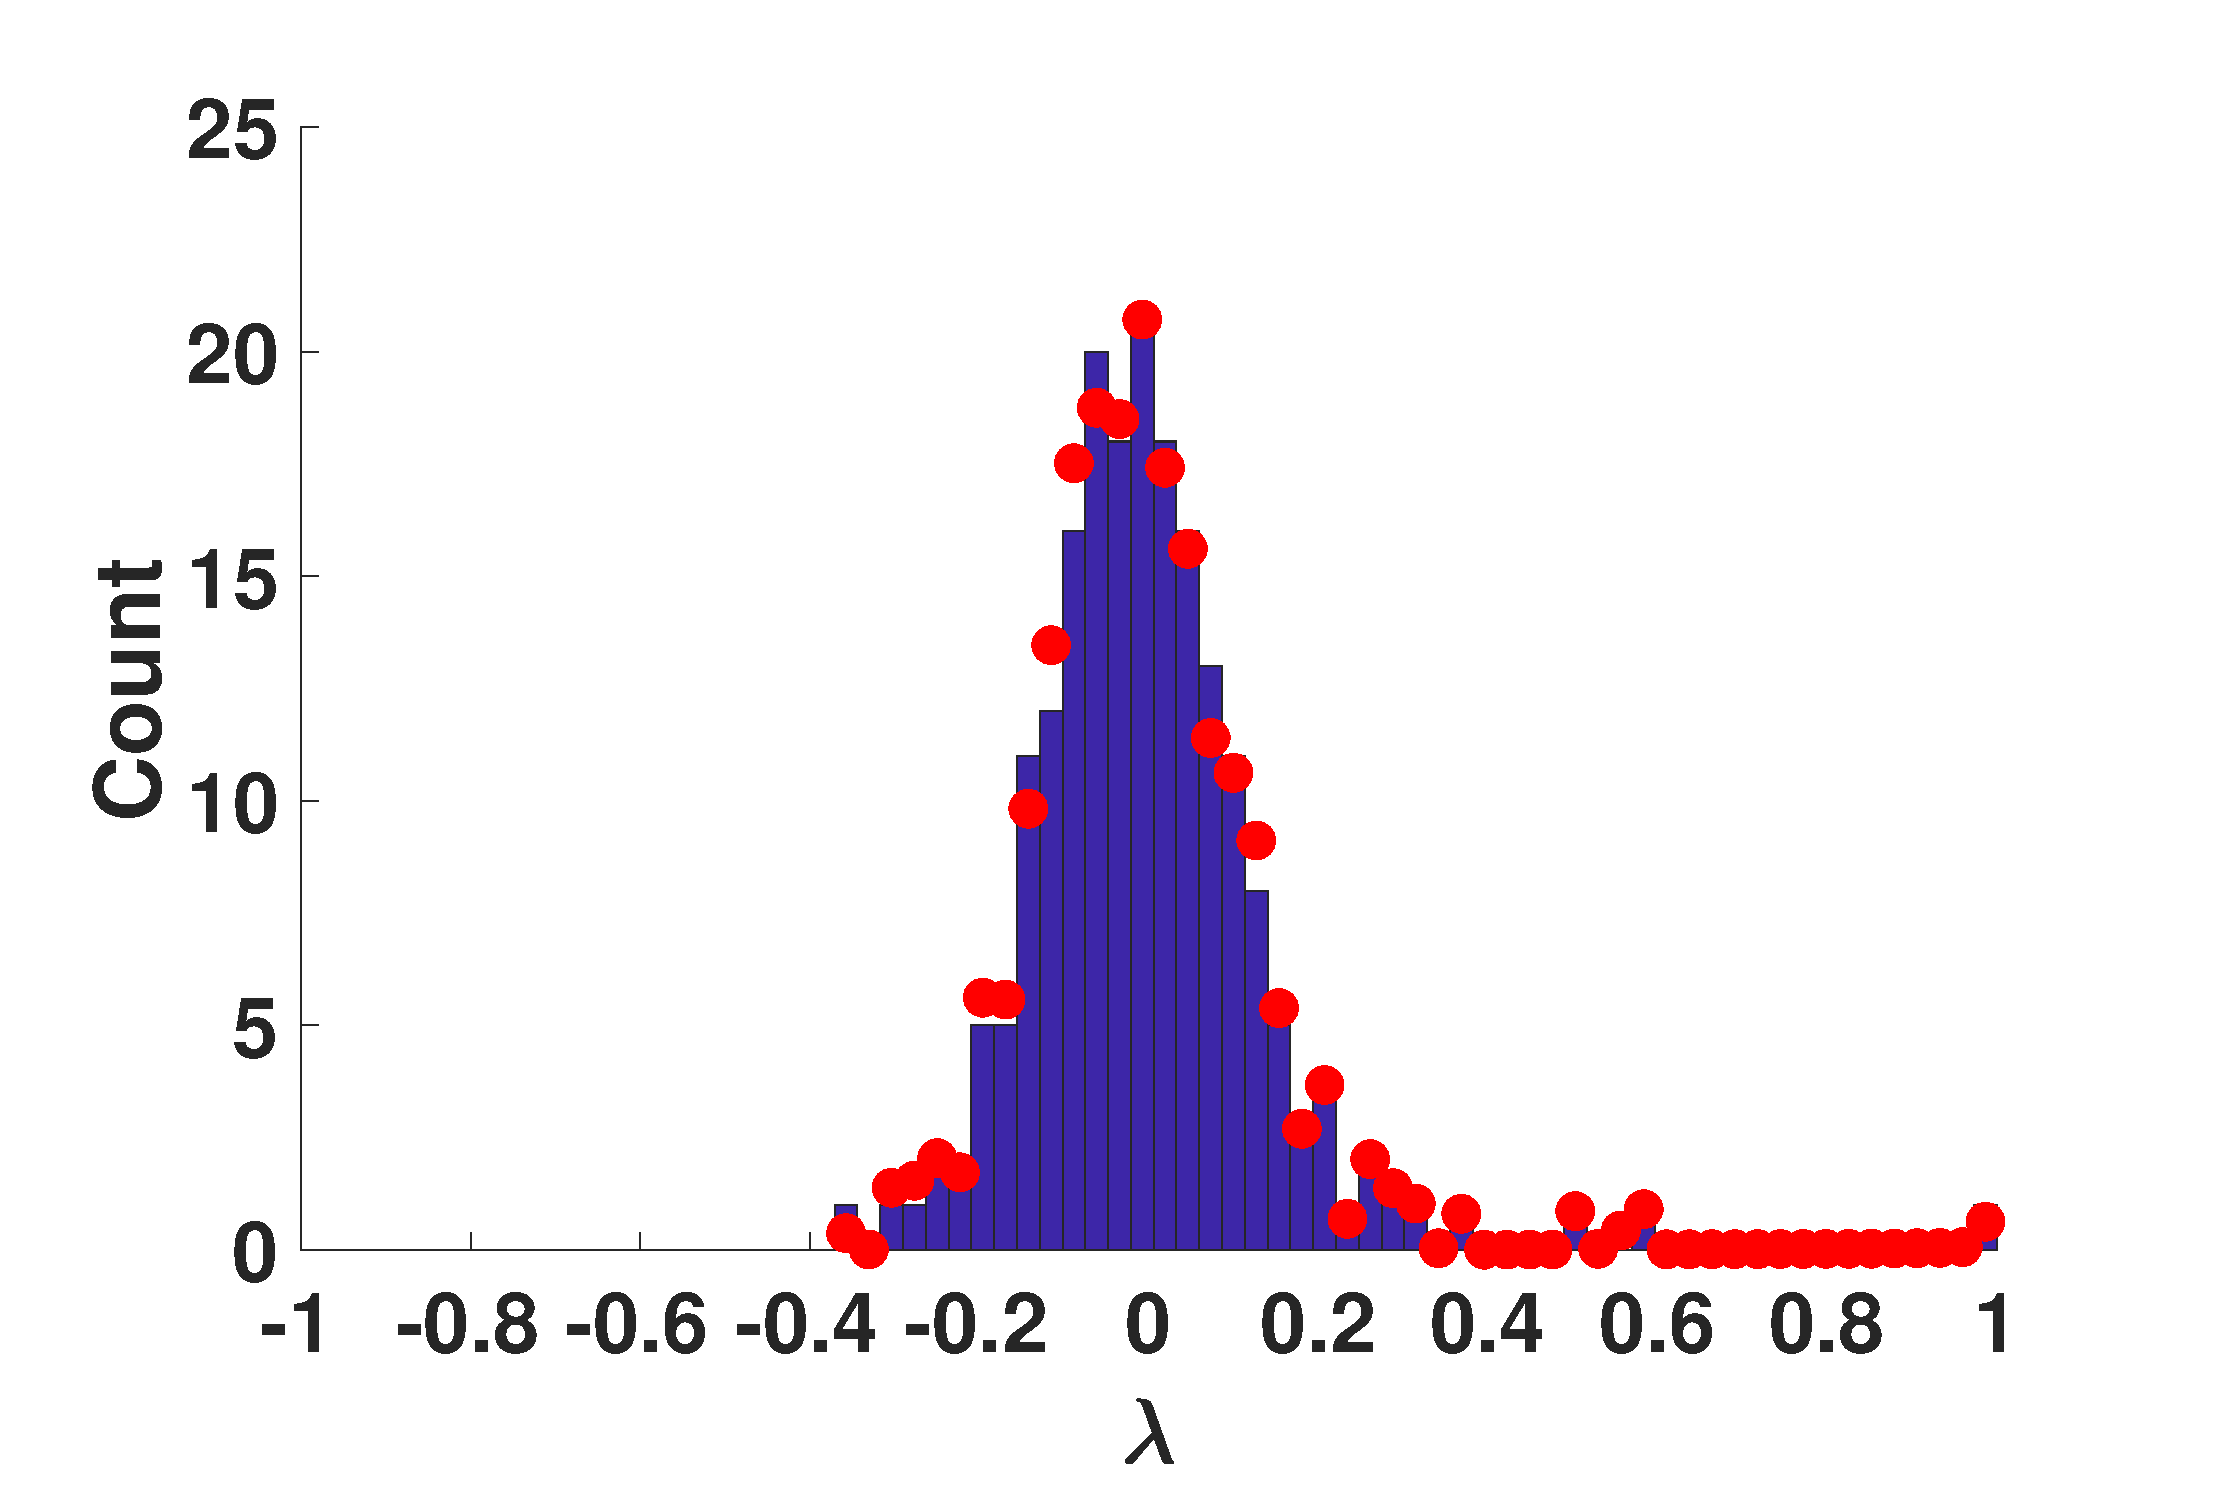
\includegraphics[width=\textwidth,trim = .4cm 0.5cm 3.5cm 1.3cm,clip]
    {./ndos/pics/twitter}
    \label{fig:twitter_dos}
  \end{subfigure}
  %
  \begin{subfigure}[t]{0.19\textwidth}
    \centering  
    \captionsetup{justification=centering,font=scriptsize}
    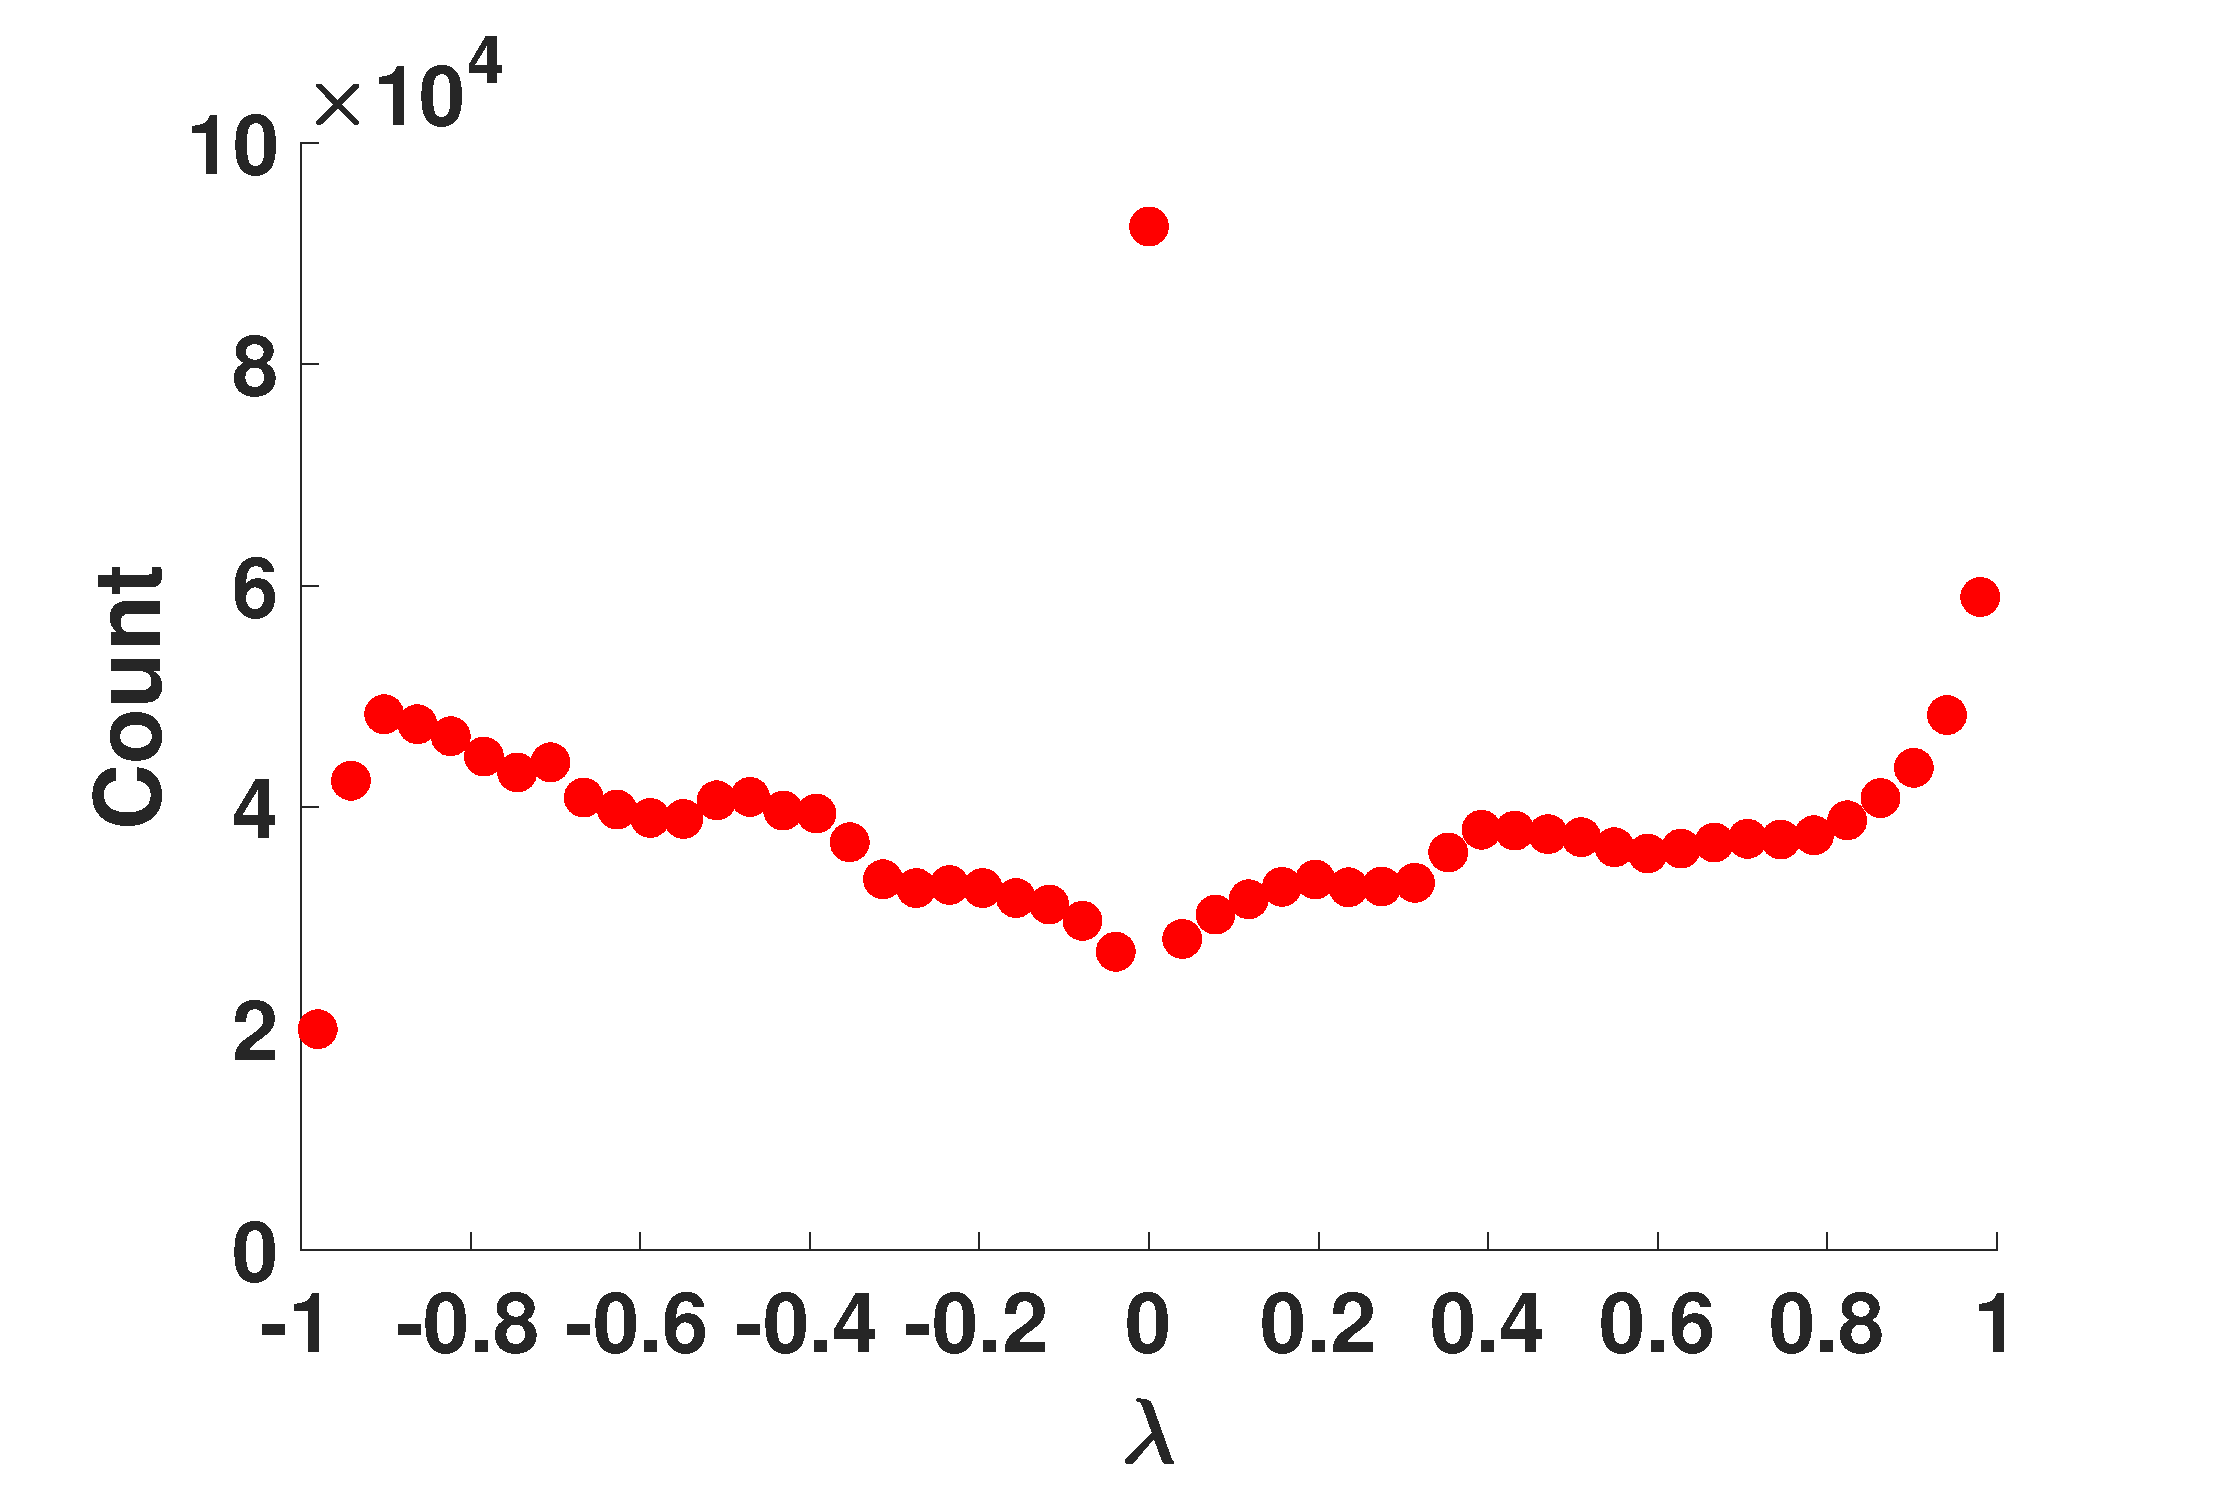
\includegraphics[width=\textwidth,trim = .4cm 0.5cm 3.5cm .3cm,clip]
    {./ndos/pics/roadca}
    \label{fig:roadca_dos}
  \end{subfigure}
  %
  \begin{subfigure}[t]{0.19\textwidth}
    \centering  
    \captionsetup{justification=centering,font=scriptsize}
    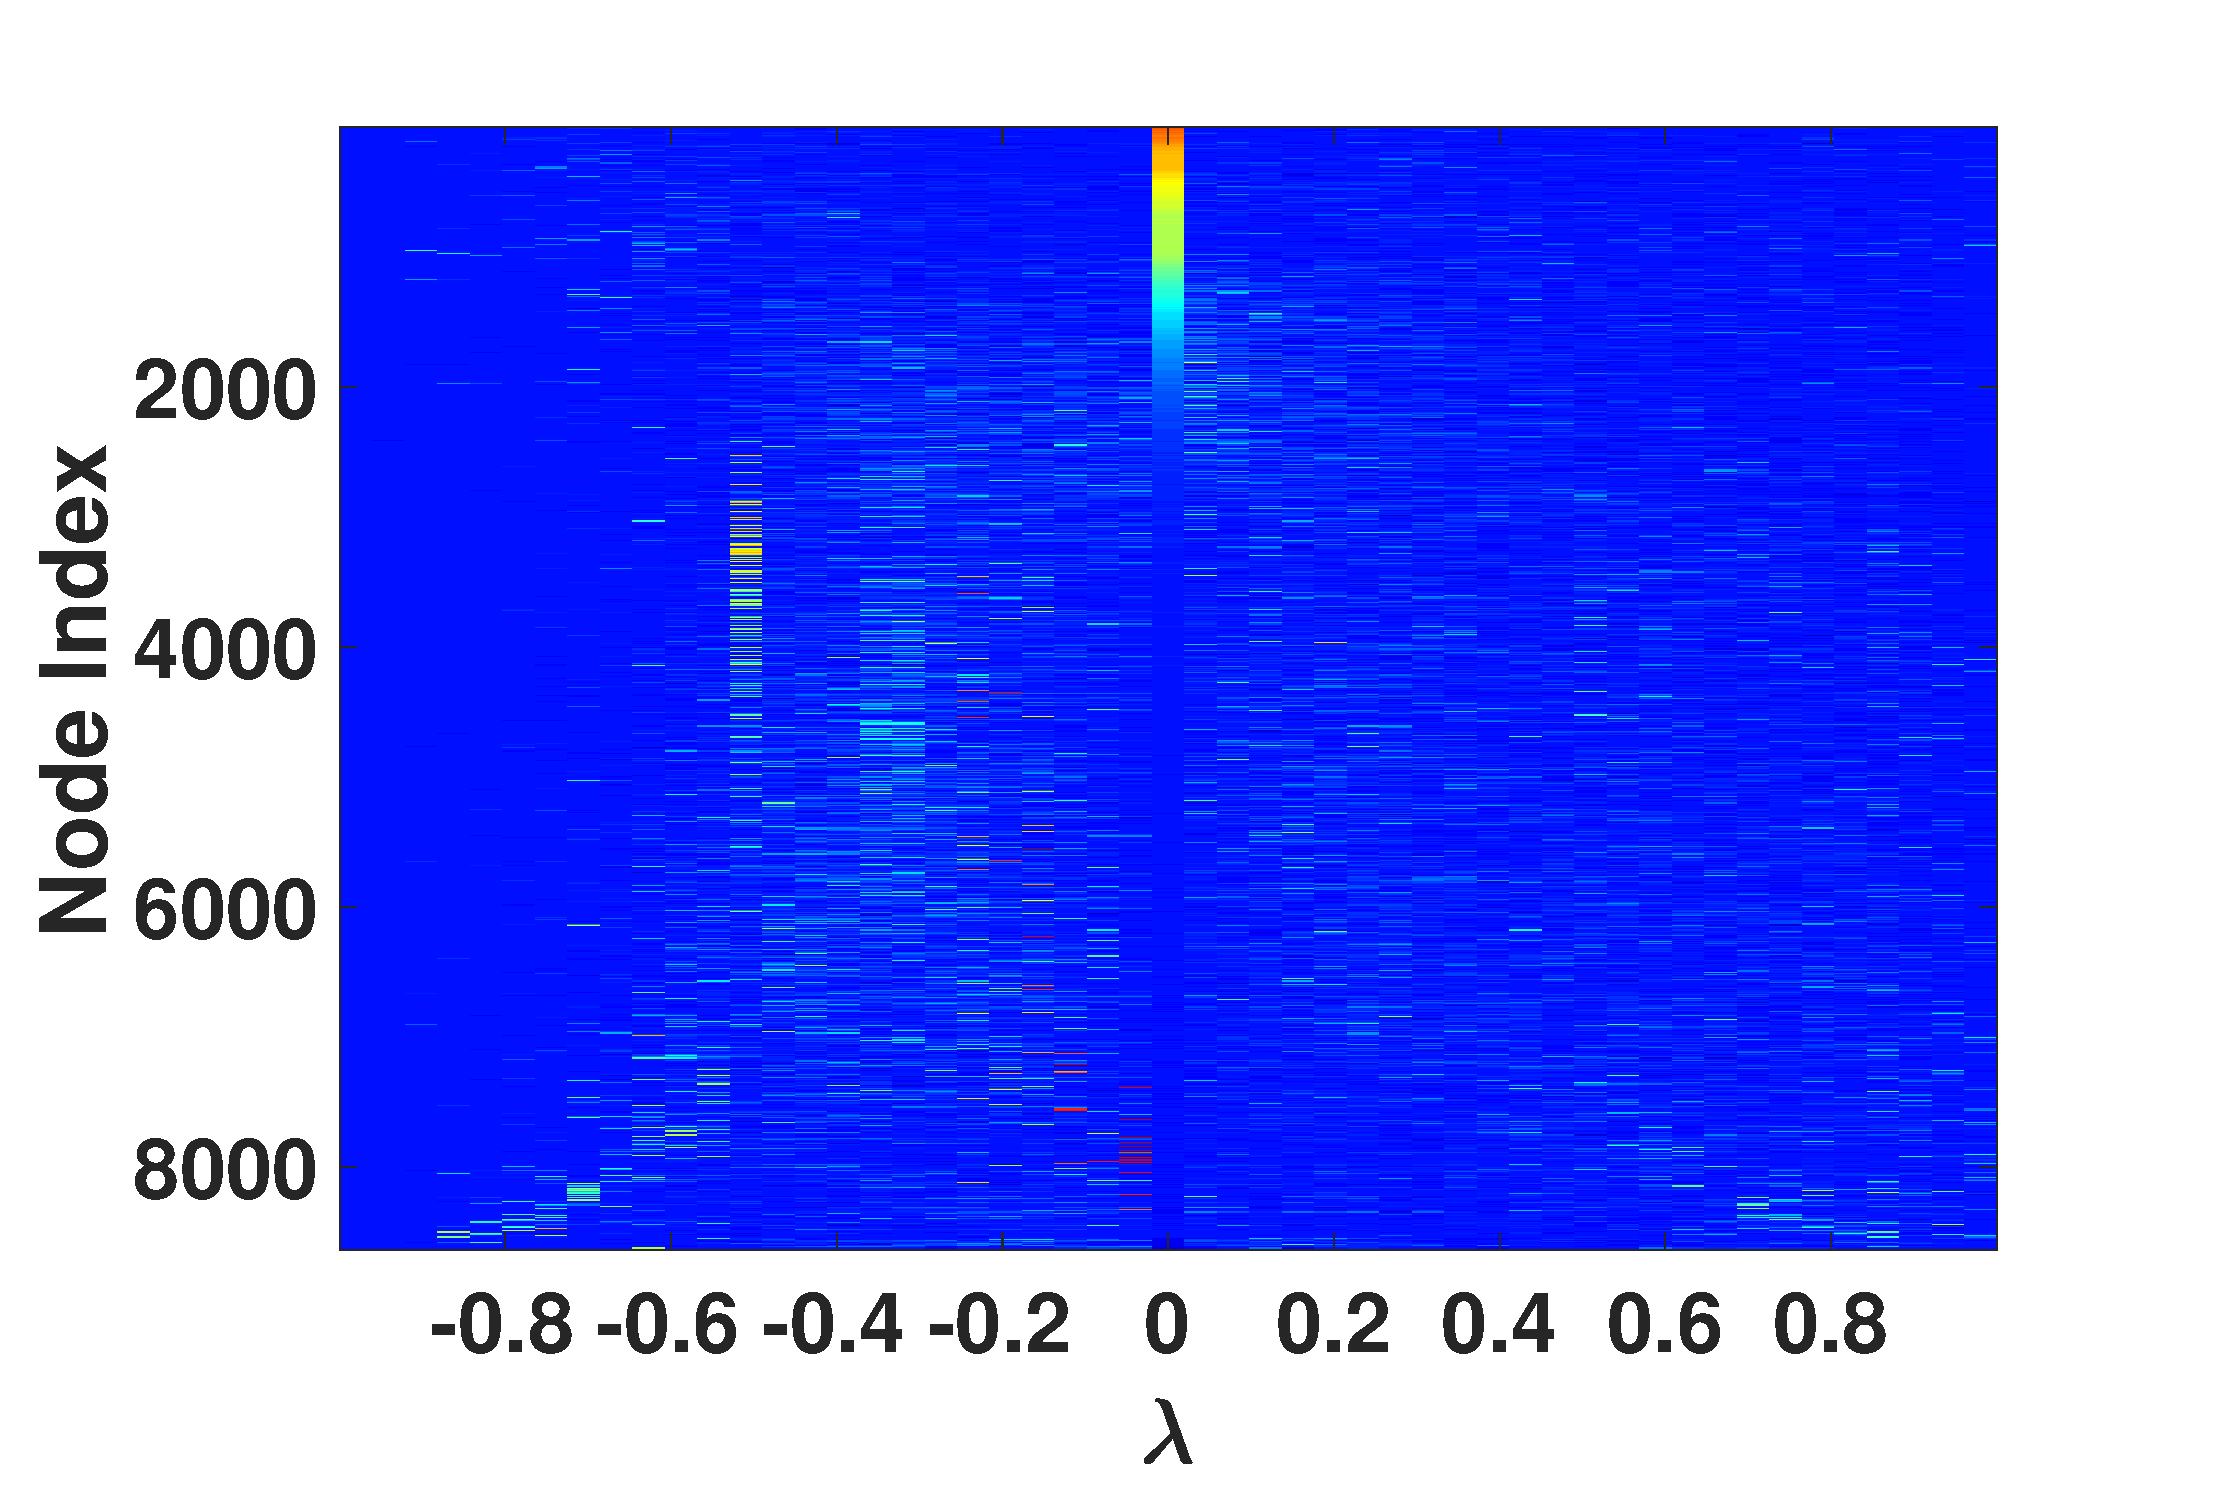
\includegraphics[width=\textwidth,trim = .4cm 0.5cm 3.5cm 1.3cm,clip]
    {./ndos/pics/hepth_ldos}
    \caption{HepTh Collaboration Network}
    \label{fig:hepth_ldos}
  \end{subfigure}
  %
  \begin{subfigure}[t]{0.19\textwidth}
    \centering  
    \captionsetup{justification=centering,font=scriptsize}
    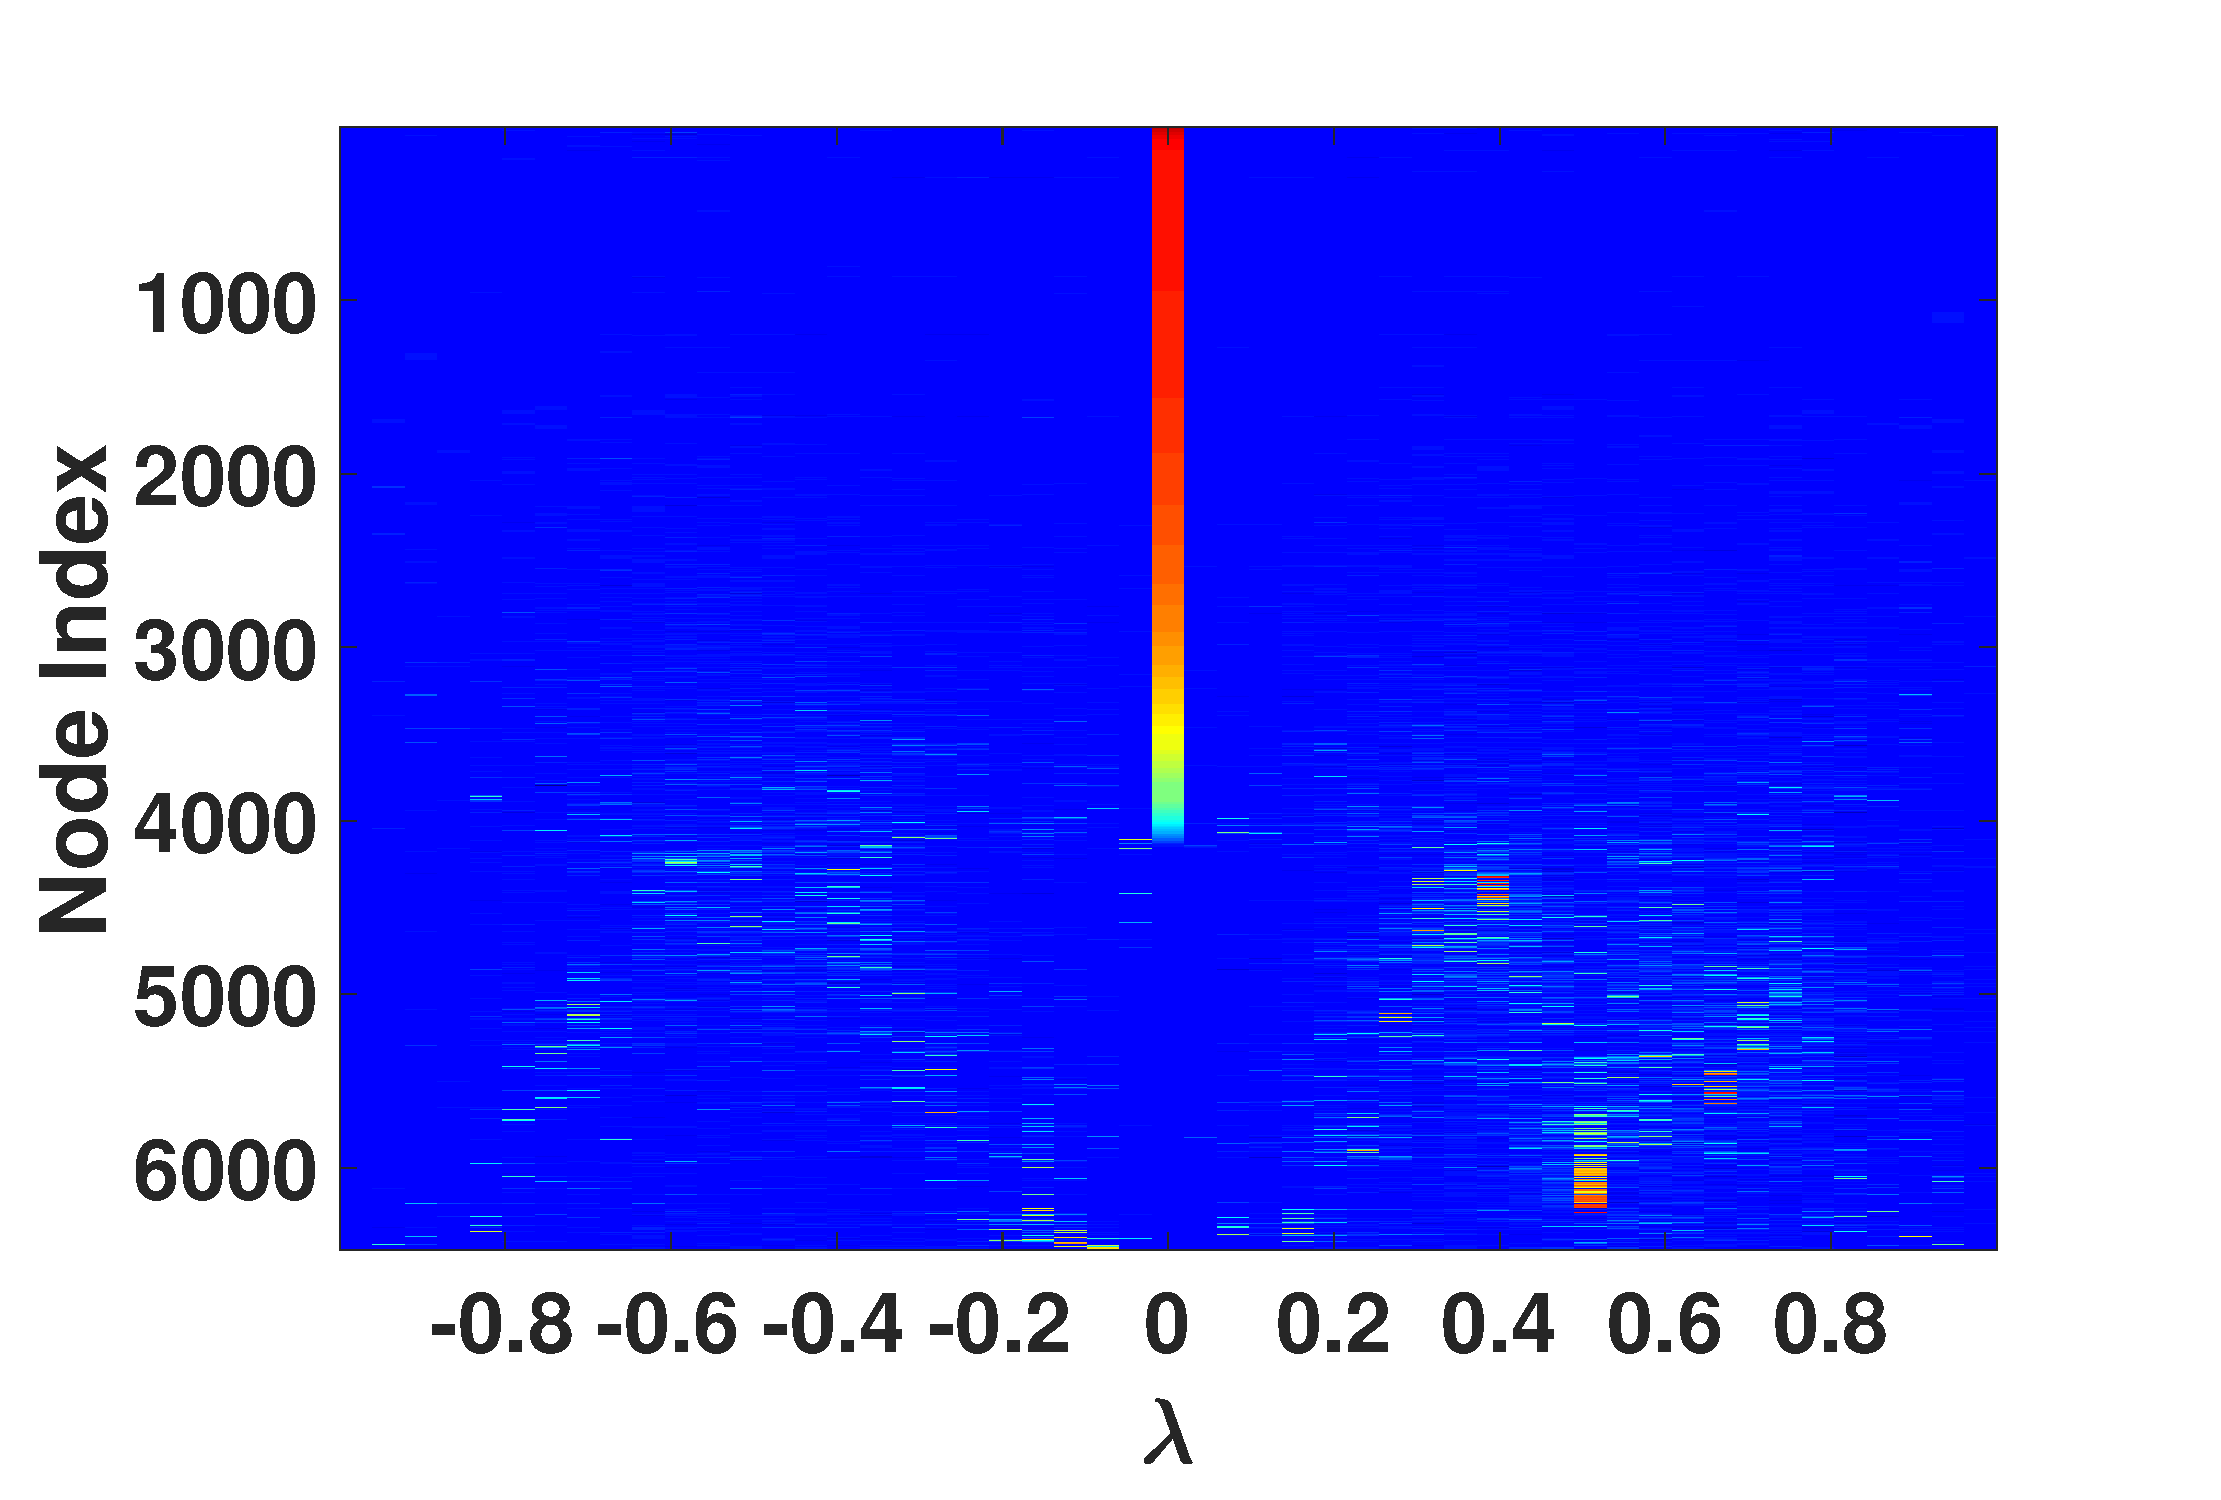
\includegraphics[width=\textwidth,trim = .4cm 0.5cm 3.5cm 1.3cm,clip]
    {./ndos/pics/as20000102_ldos}
    \caption{Autonomous System Network (2000)}
    \label{fig:as2_ldos}
  \end{subfigure}
  %
  \begin{subfigure}[t]{0.19\textwidth}
    \centering  
    \captionsetup{justification=centering,font=scriptsize}
    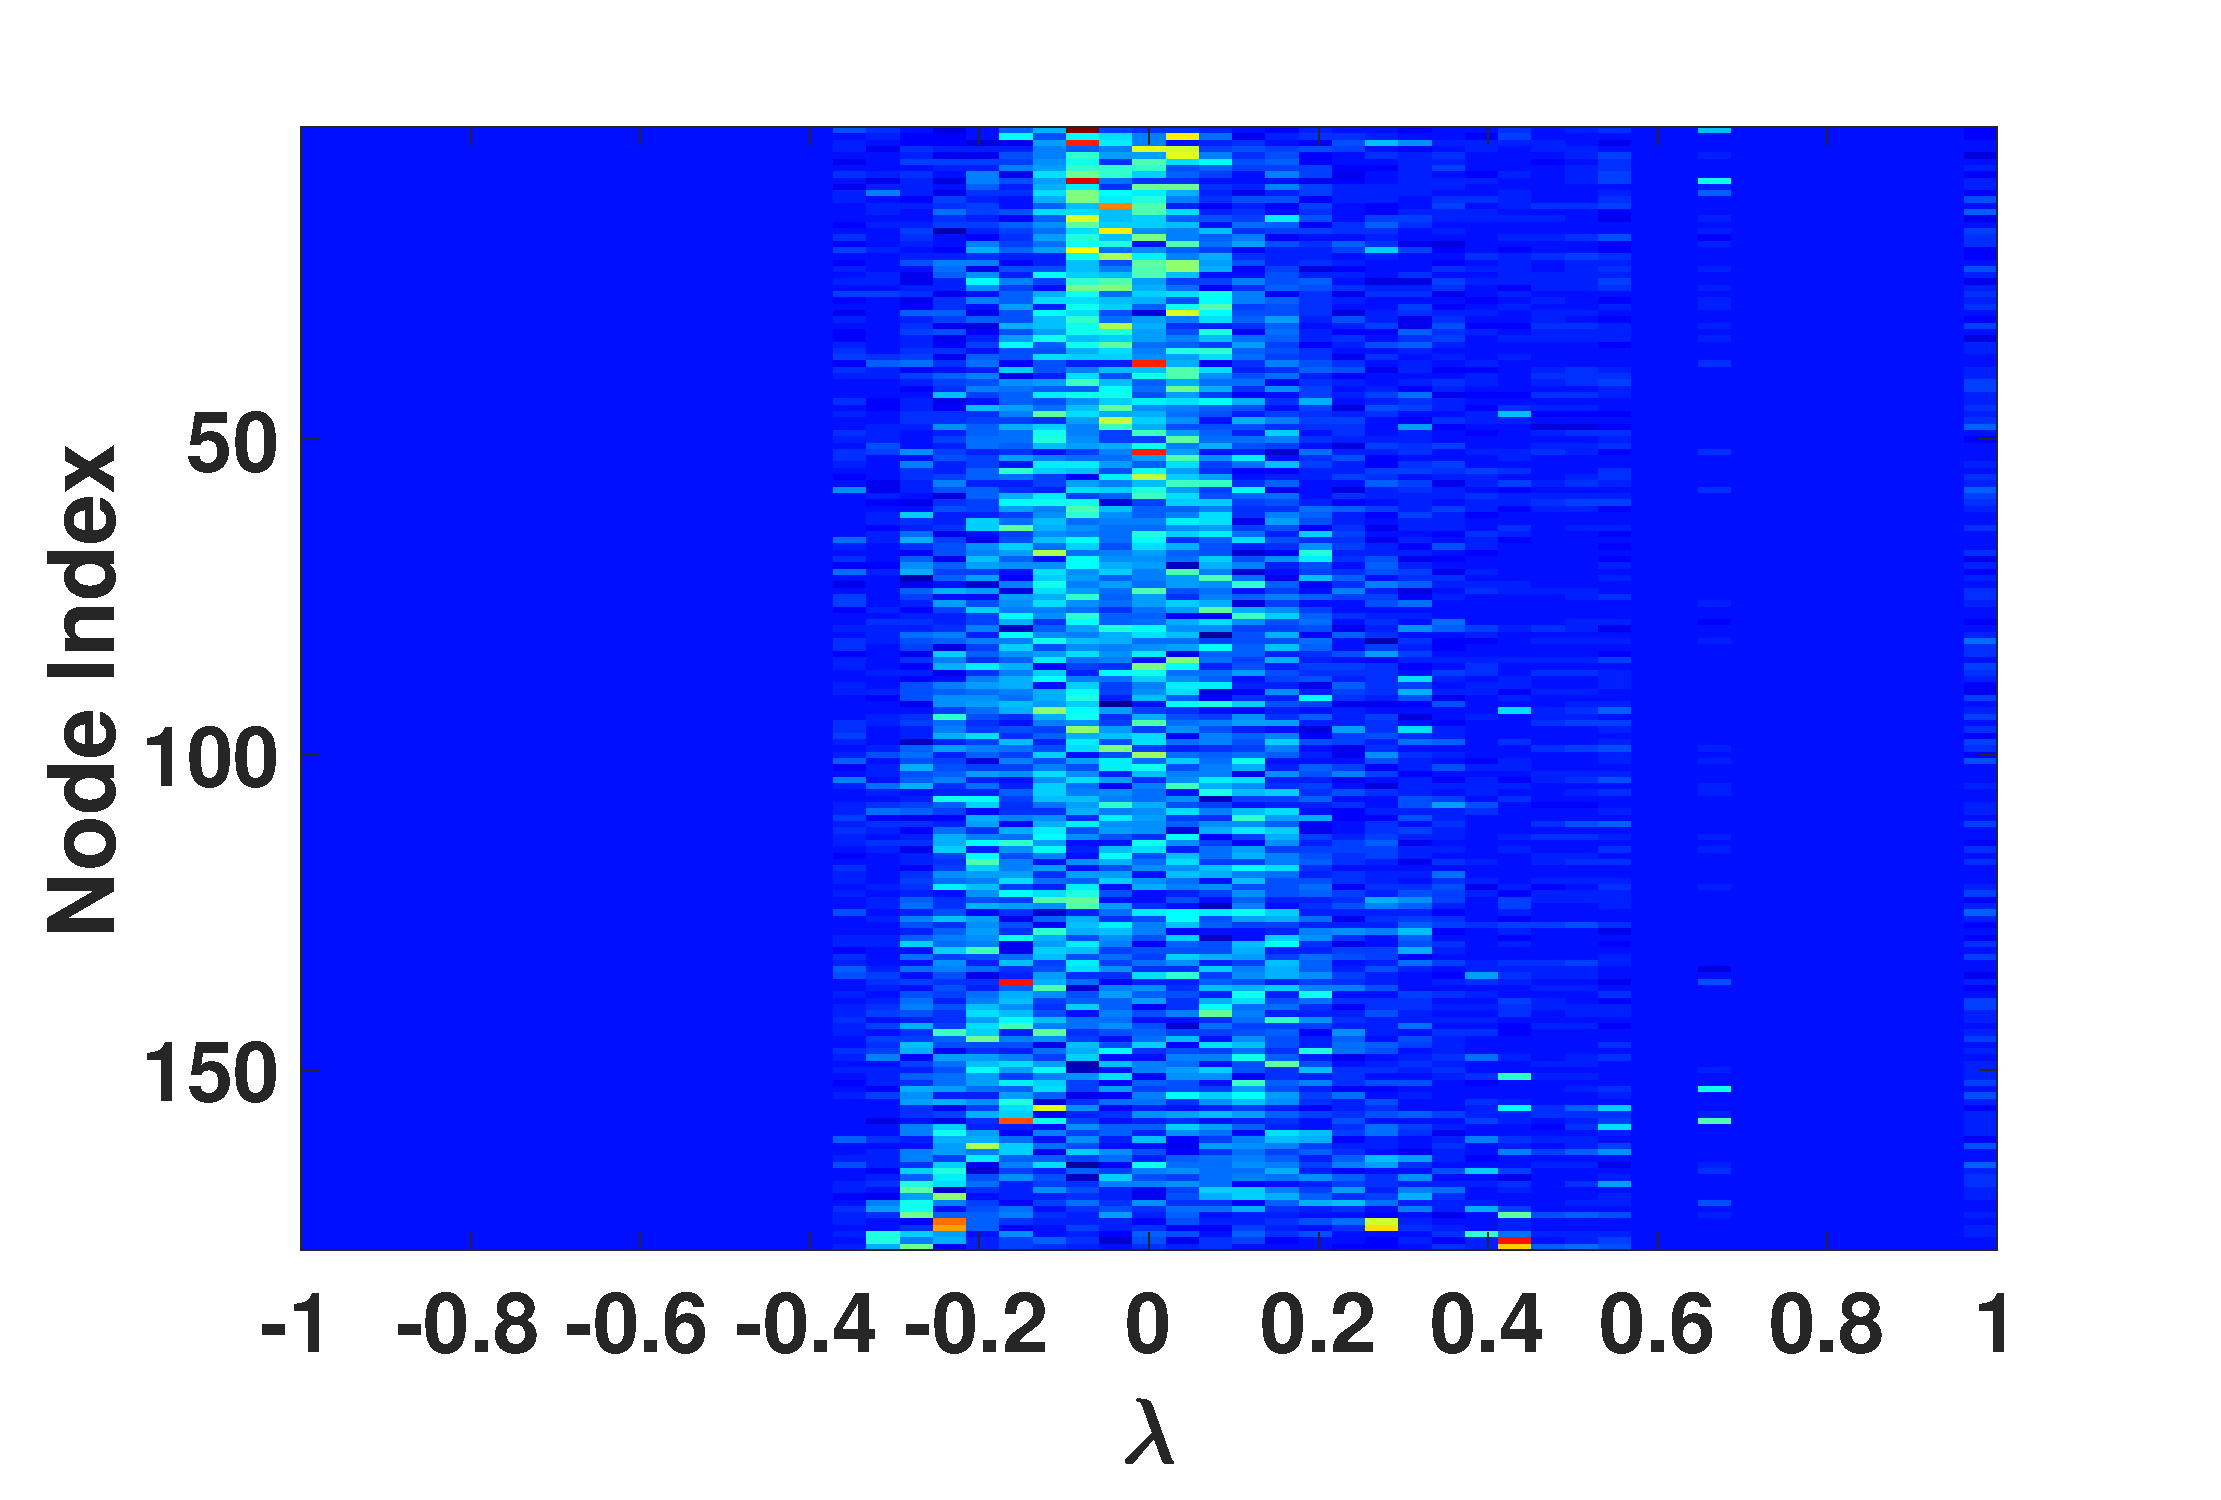
\includegraphics[width=\textwidth,trim = .4cm 0.5cm 3.5cm 1.3cm,clip]
    {./ndos/pics/hp_ldos}{}
    \caption{Harry Potter Characters Network}
    \label{fig:hp_ldos}
  \end{subfigure}
  %
  \begin{subfigure}[t]{0.19\textwidth}
    \centering  
    \captionsetup{justification=centering,font=scriptsize}
    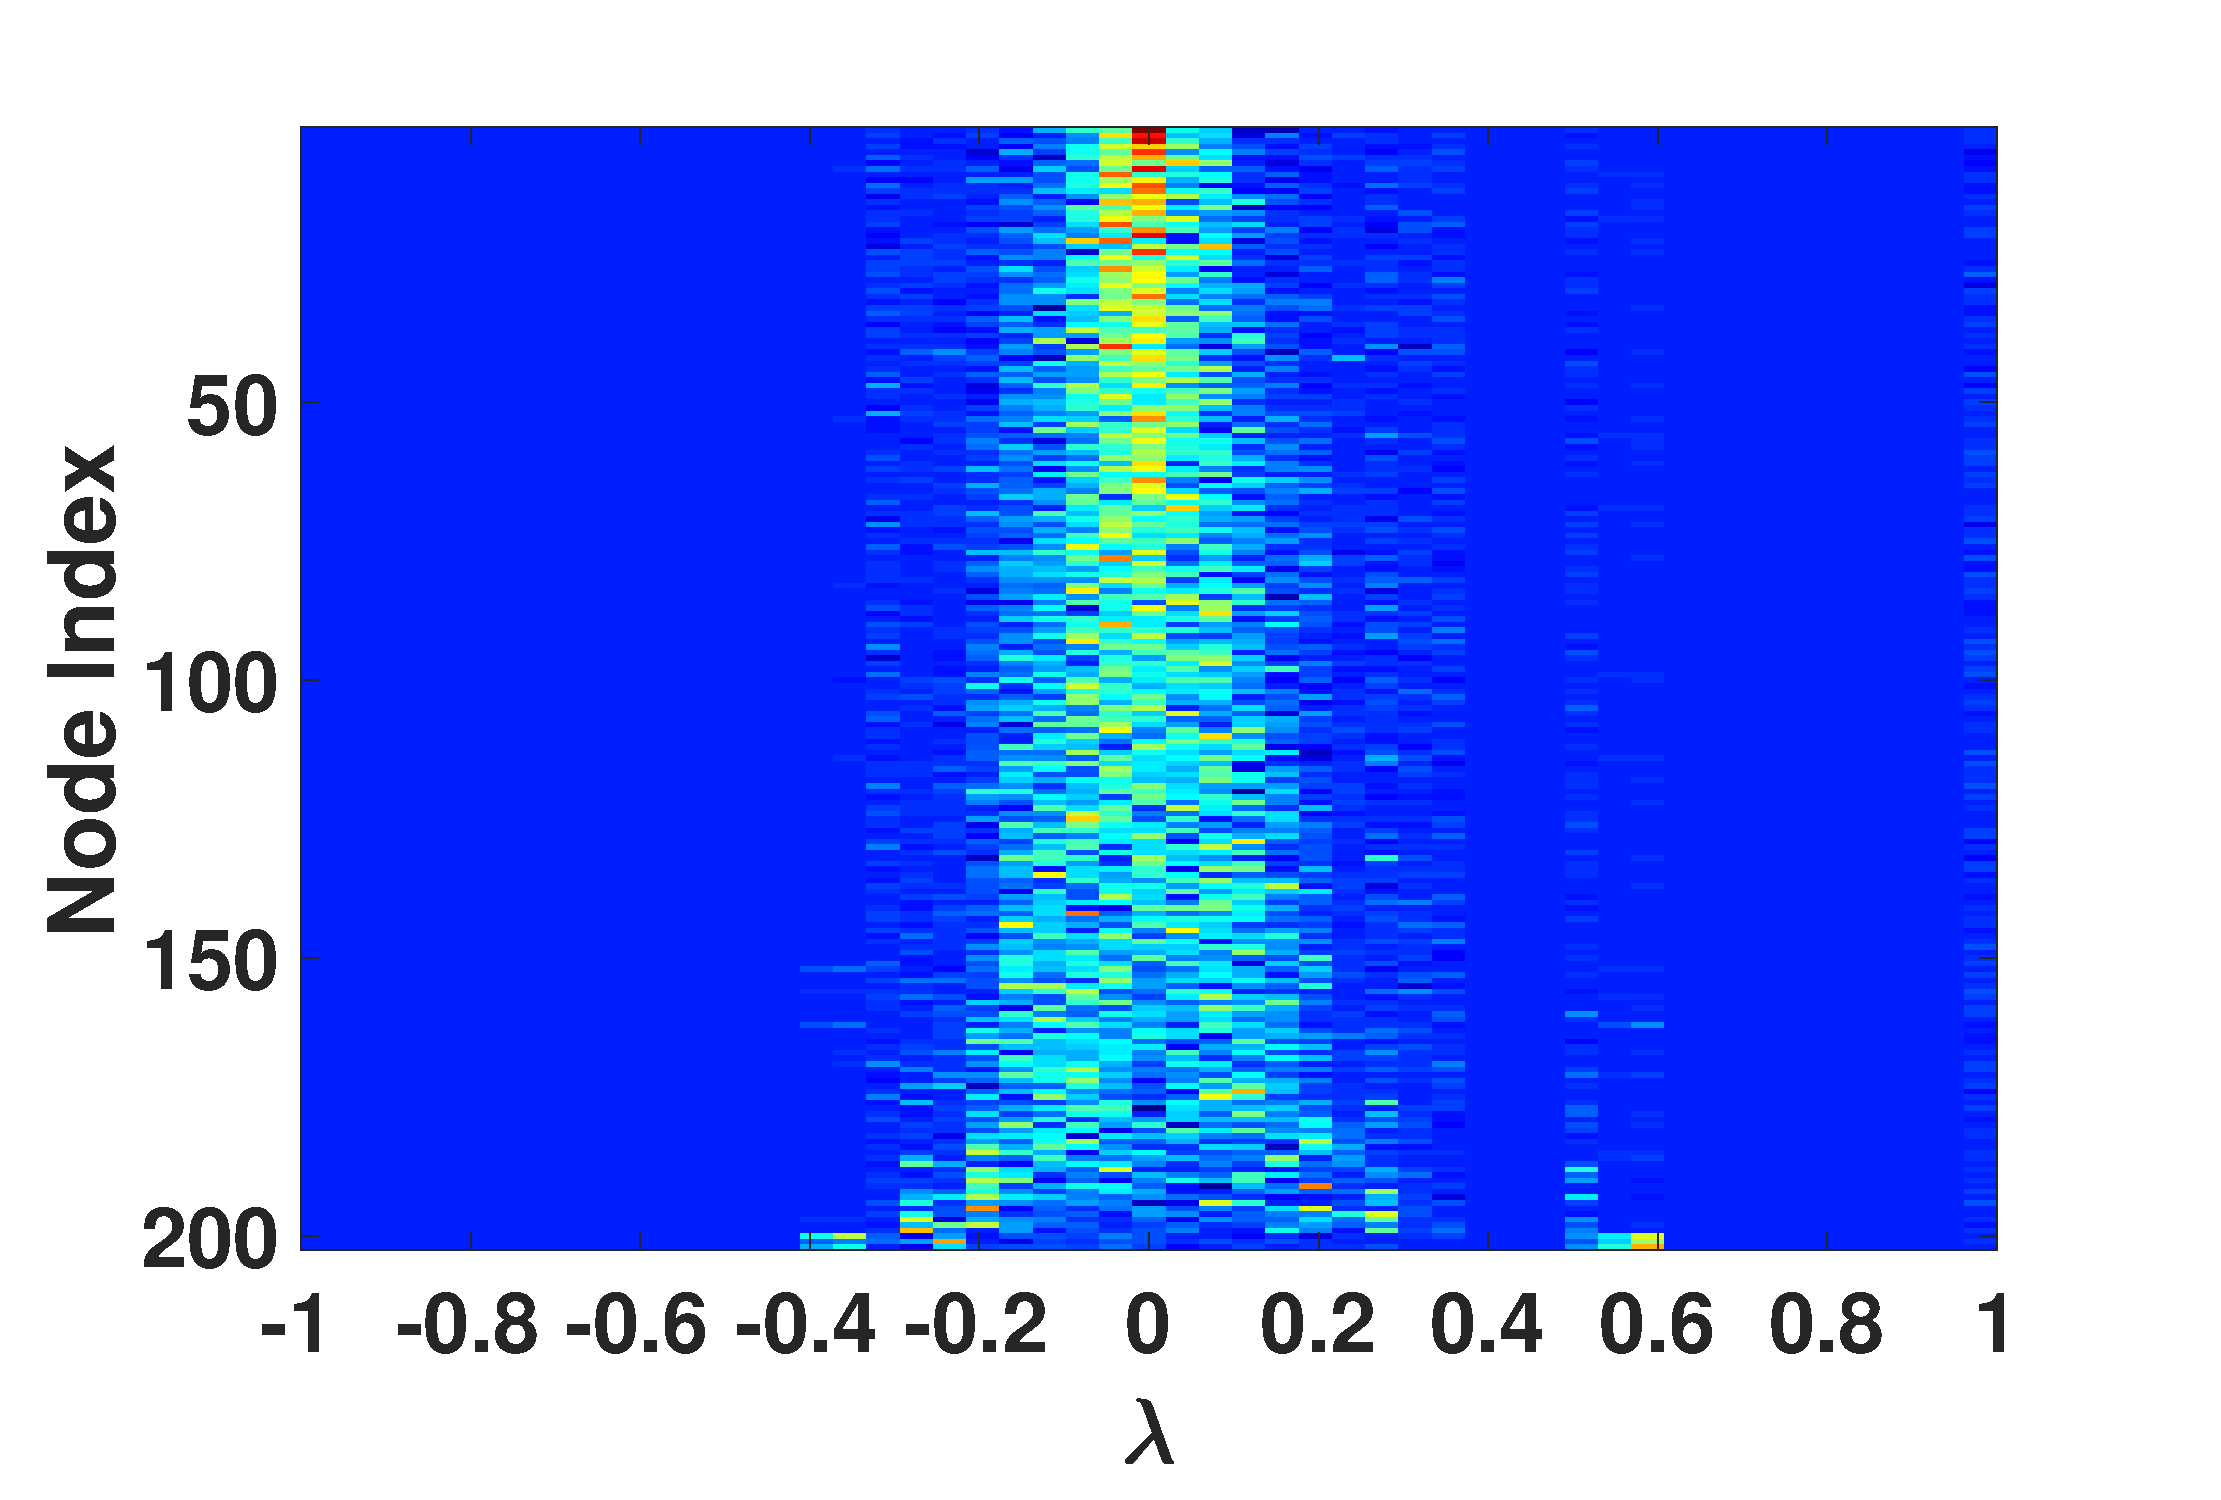
\includegraphics[width=\textwidth,trim = .4cm 0.5cm 3.5cm 1.3cm,clip]
    {./ndos/pics/twitter_ldos}
    \caption{Twitter Ego \\Networks}
    \label{fig:twitter_ldos}
  \end{subfigure}
  %
  \begin{subfigure}[t]{0.19\textwidth}
    \centering  
    \captionsetup{justification=centering,font=scriptsize}
    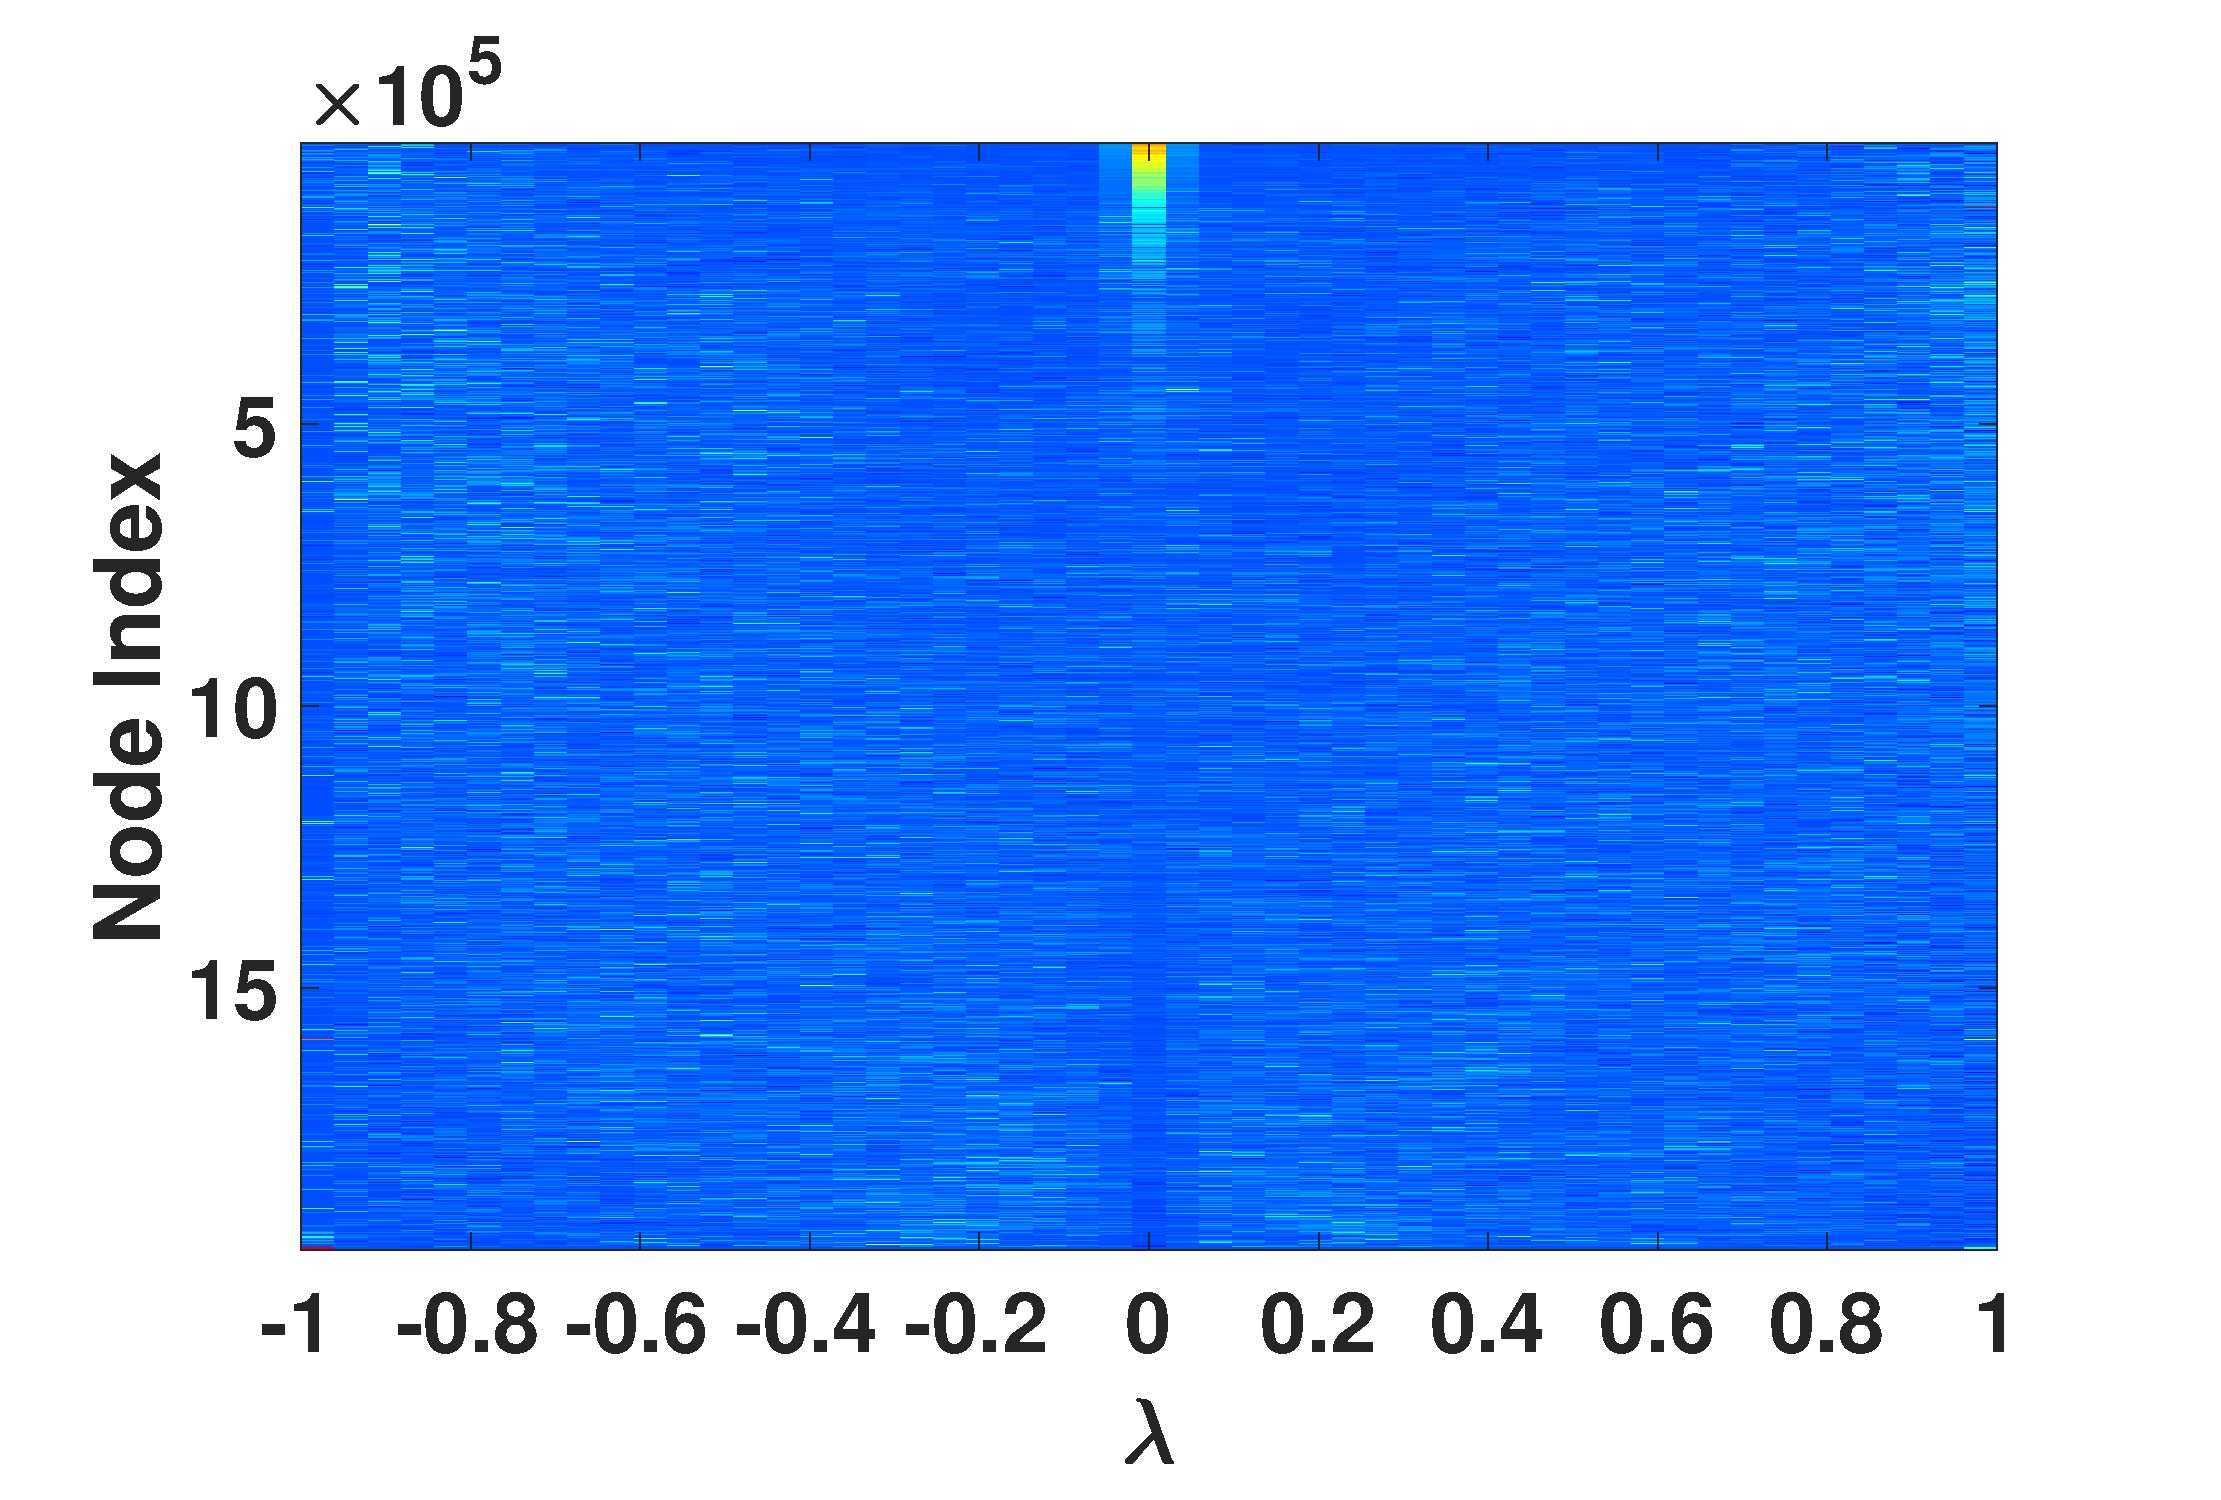
\includegraphics[width=\textwidth,trim = .4cm 0.5cm 3.5cm 0.3cm,clip]
    {./ndos/pics/roadca_ldos}
    \caption{California Road Network}
    \label{fig:roadca_ldos}
  \end{subfigure}
  \caption{DOS(top)/PDOS(bottom) histograms for the normalized adjacency of 10
  networks from five domains. For DOS, blue bars are the true spectrum, and red
  points are from KPM ($500$ moments and $20$ Hadamard probes). For PDOS, the
  spectral histograms of all nodes are aligned vertically. Red indicates high
  weight around an eigenvalue, and blue indicates low weight. The true spectrum
  for the California Road Network (\ref{fig:roadca_ldos}) is omitted, as it is
  too large to compute exactly (1,965,206 nodes).}\label{fig:gallery}
\end{figure}

\subsection{Computation Time}

In this experiment, we show the scaling of our methods by applying them to
graphs of varying size of nodes, edges, and sparsity patterns. Rather than
computation power, the memory cost of loading a graph with 100M-1B edges is more
often the constraint. Hence, we report runtimes for a Python version on a Google
Cloud instance with 200GB memory and an Intel Xeon E5 v3 CPU at 2.30GHz.

The datasets we use are obtained from the SNAP repository~\cite{snapnets}. For
each graph, we compute the first $10$ Chebyshev moments using KPM with $20$
probe vectors. Most importantly, the cost for each moment is independent of the
total number of moments we compute. \cref{tab:scaling} reports number of
nodes, number of edges, average degree of nodes, and the average runtime for
computing each moment. We can observe that the runtime is in accordance with
the theoretical complexity $\calO(N_z(\abs{V} + \abs{E}))$. For the Friendster
social network with about 1.8 billion edges, computing each moment takes about
1000 seconds to compute, which means we could obtain a rough approximation to
its spectrum within a day. As the dominant cost is matrix-matrix multiplication
and we use several probe vectors, our approach has ample opportunity for
parallel computation.
\begin{table}[ht]
  \begin{center}
  \captionsetup{width=.8\textwidth}
  \caption{Average Computation Time per Chebyshev Moment for Graphs from the
  SNAP Repository\textsuperscript{$\alpha$}.}\label{tab:scaling}
  \begin{threeparttable}
    \begin{tabular}{r r r r r}
      \toprule
      Network & \# Nodes &\# Edges & Avg.\ Deg.\ & Time (s) \\ \midrule
      Facebook & 4,039 & 88,234 & 43.69 & 0.007\\
      AstroPh & 18,772 & 198,110 & 21.11 & 0.028\\
      Enron & 36,692 & 183,831 & 10.02 & 0.046\\
      Gplus & 107,614 & 13,673,453 & 254.12 & 1.133\\
      Amazon & 334,863 & 925,872 & 5.53 & 0.628\\
      Neuron & 1,018,524 & 24,735,503 & 48.57 & 9.138\\
      RoadNetCA & 1,965,206 & 2,766,607 & 2.82 & 2.276\\
      Orkut & 3,072,441 & 117,185,083 & 76.28 & 153.7\\
      LiveJournal & 3,997,962 & 34,681,189 & 17.35 & 14.52 \\
      Friendster & 65,608,366 & 1,806,067,135 & 55.06 & 1,017\\
      \bottomrule
    \end{tabular}
    \begin{tablenotes}
      \item[$\alpha$]$20$ probe vectors are used throughout the experiment. The
      runtime is averaged over 5 moments.
    \end{tablenotes}
  \end{threeparttable}
  \end{center}
\end{table}

\subsection{Model Verification}

In this experiment, we investigate the spectrum for some of the popular graph
models, and whether they resemble the behavior of real-world data. Two of the
most popular models used to describe real-world graphs are the scale-free model 
\cite{barabasi1999emergence} and the small-world model 
\cite{watts1998collective}. \citet{farkas2001spectra} has analyzed
the spectrum of the adjacency matrix; we instead consider the normalized
adjacency.

The scale-free model grows a random graph with the preferential attachment
process, starting from an initial seed graph and adding one node and $m$ edges
at every step. \cref{fig:ba} shows spectral histograms for this model with
$5000$ nodes and different choices of $m$. When $m=1$, the generated graph has
abundant local motifs like many sparse real-world graphs. By searching in PDOS
for the nodes that have high weight at the two spikes, we find node-doubles 
($\lambda=0)$ and singly-attached chains ($\lambda=\pm 1/\sqrt{2}$). When $m=5$,
the graph is denser, without any particular motifs, resulting in an
approximately semicircular spectral distribution.

\begin{figure}[ht]
  \begin{subfigure}{0.47\textwidth}
    \centering  
    \captionsetup{justification=centering}
    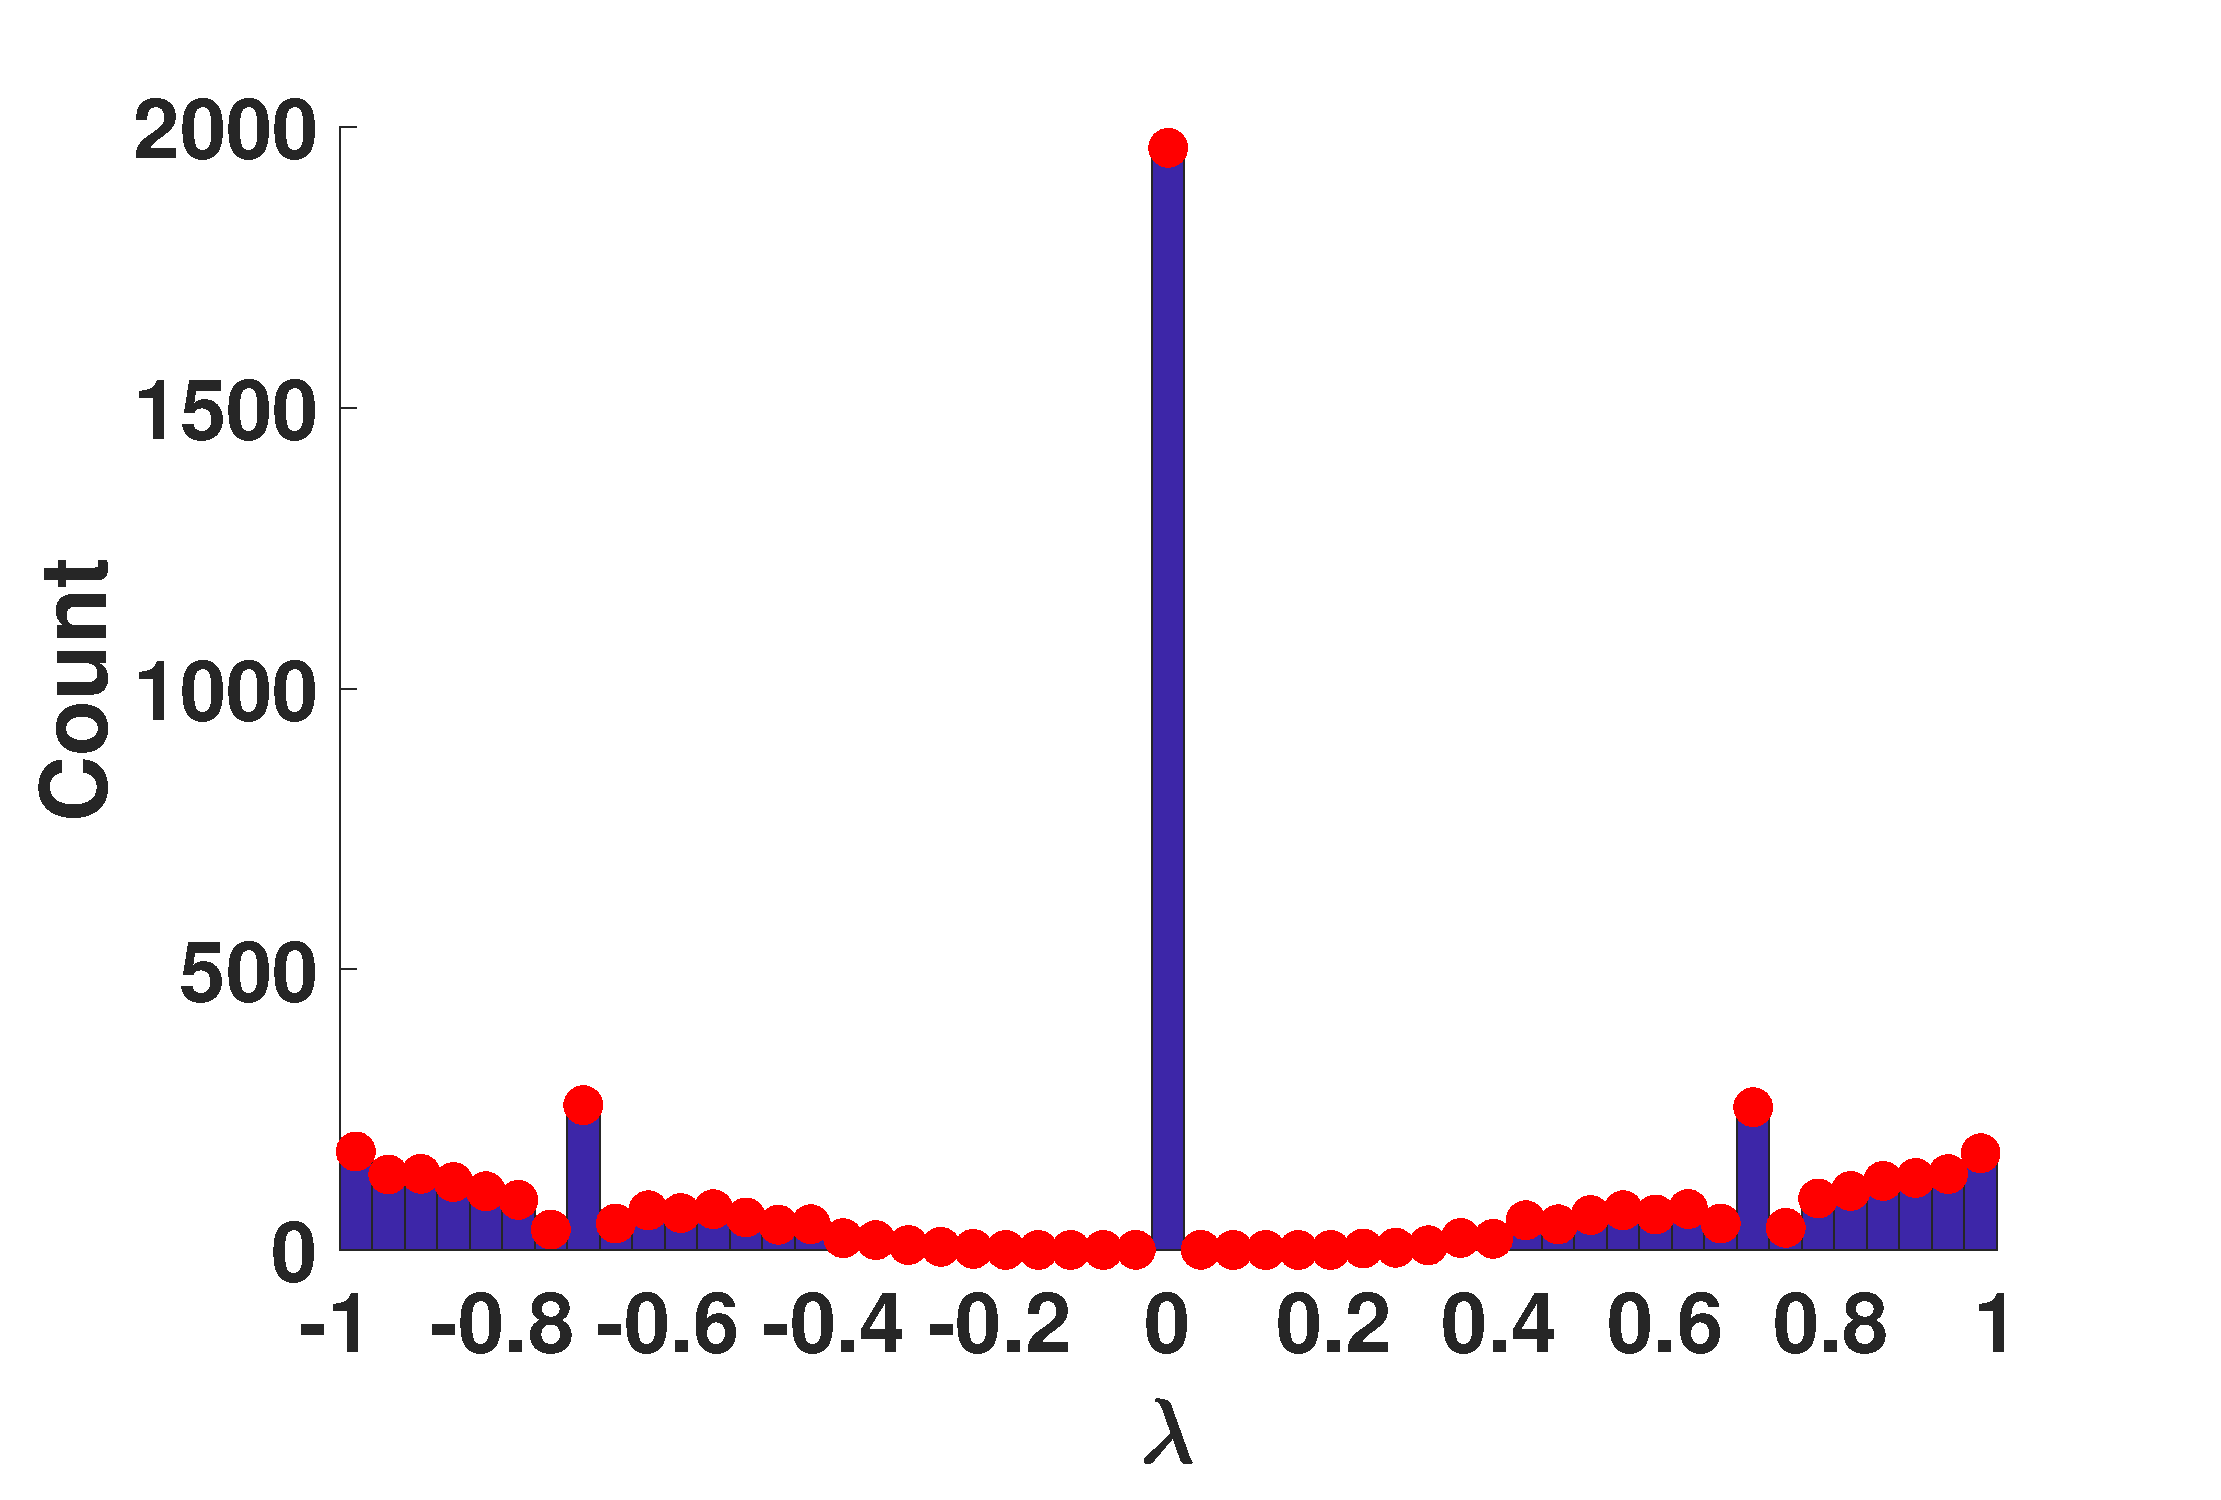
\includegraphics[width=\textwidth,trim = .4cm 0.5cm 3.5cm 1.3cm,clip]
    {./ndos/pics/ba_sparse}
    \caption{$m = 1$}\label{fig:ba_sparse}
  \end{subfigure}
  %
  \begin{subfigure}{0.47\textwidth}
    \centering
    \captionsetup{justification=centering}
    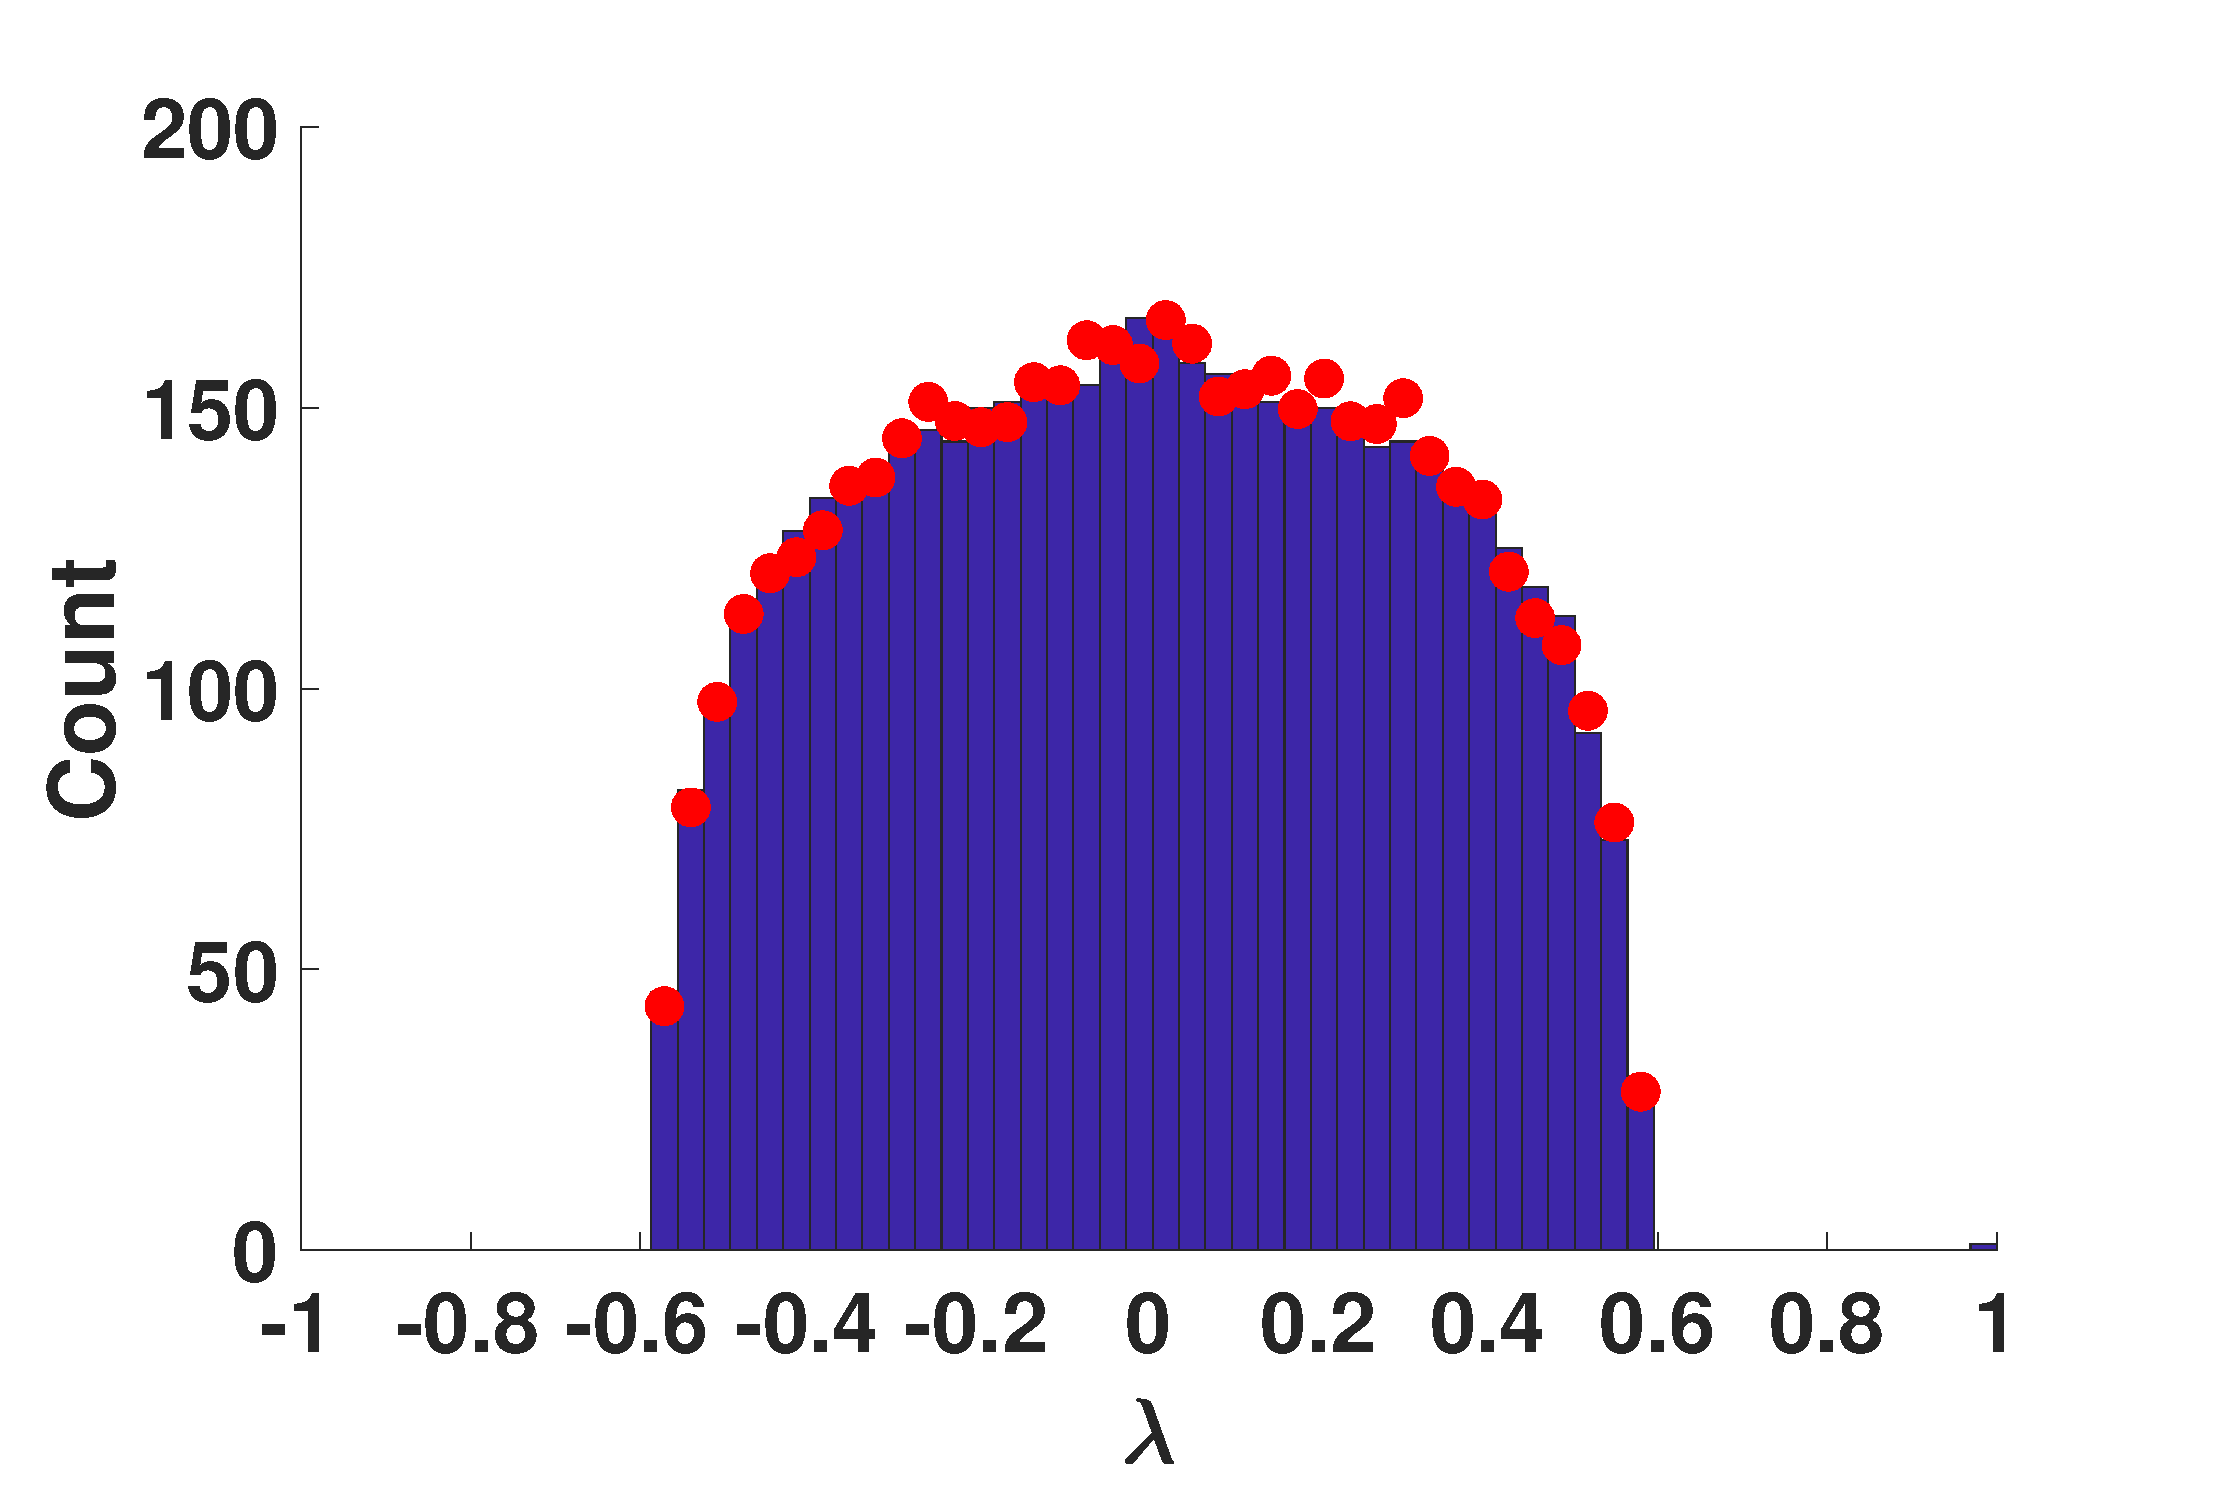
\includegraphics[width=\textwidth,trim = .4cm 0.5cm 3.5cm 1.3cm,clip]
    {./ndos/pics/ba_dense}
    \caption{$m = 5$}\label{fig:ba_dense}
  \end{subfigure}
  \caption{Spectral histogram for scale-free model with $5000$ nodes and
  different $m$. Blue bars are the real spectrum, red points are from KPM
  ($500$ moments and $20$ probes).} \label{fig:ba}
\end{figure}

The small-world model generates a random graph by re-wiring edges of a ring
lattice with a certain probability $p$. Here we construct these graphs on $5000$
nodes with $p=0.5$; the pattern in spectrum is insensitive for a wide range of
$p$. In \cref{fig:sw}, when the graph is sparse with $5000$ edges, the spectrum
has spikes at $0$ and $\pm 1$, indicating local symmetries, bipartite structure,
and disconnected components. With $50000$ edges, localized structures disappear
and the spectrum has narrower support.

\begin{figure}[ht]
  \begin{subfigure}{0.47\textwidth}
    \centering  
    \captionsetup{justification=centering}
    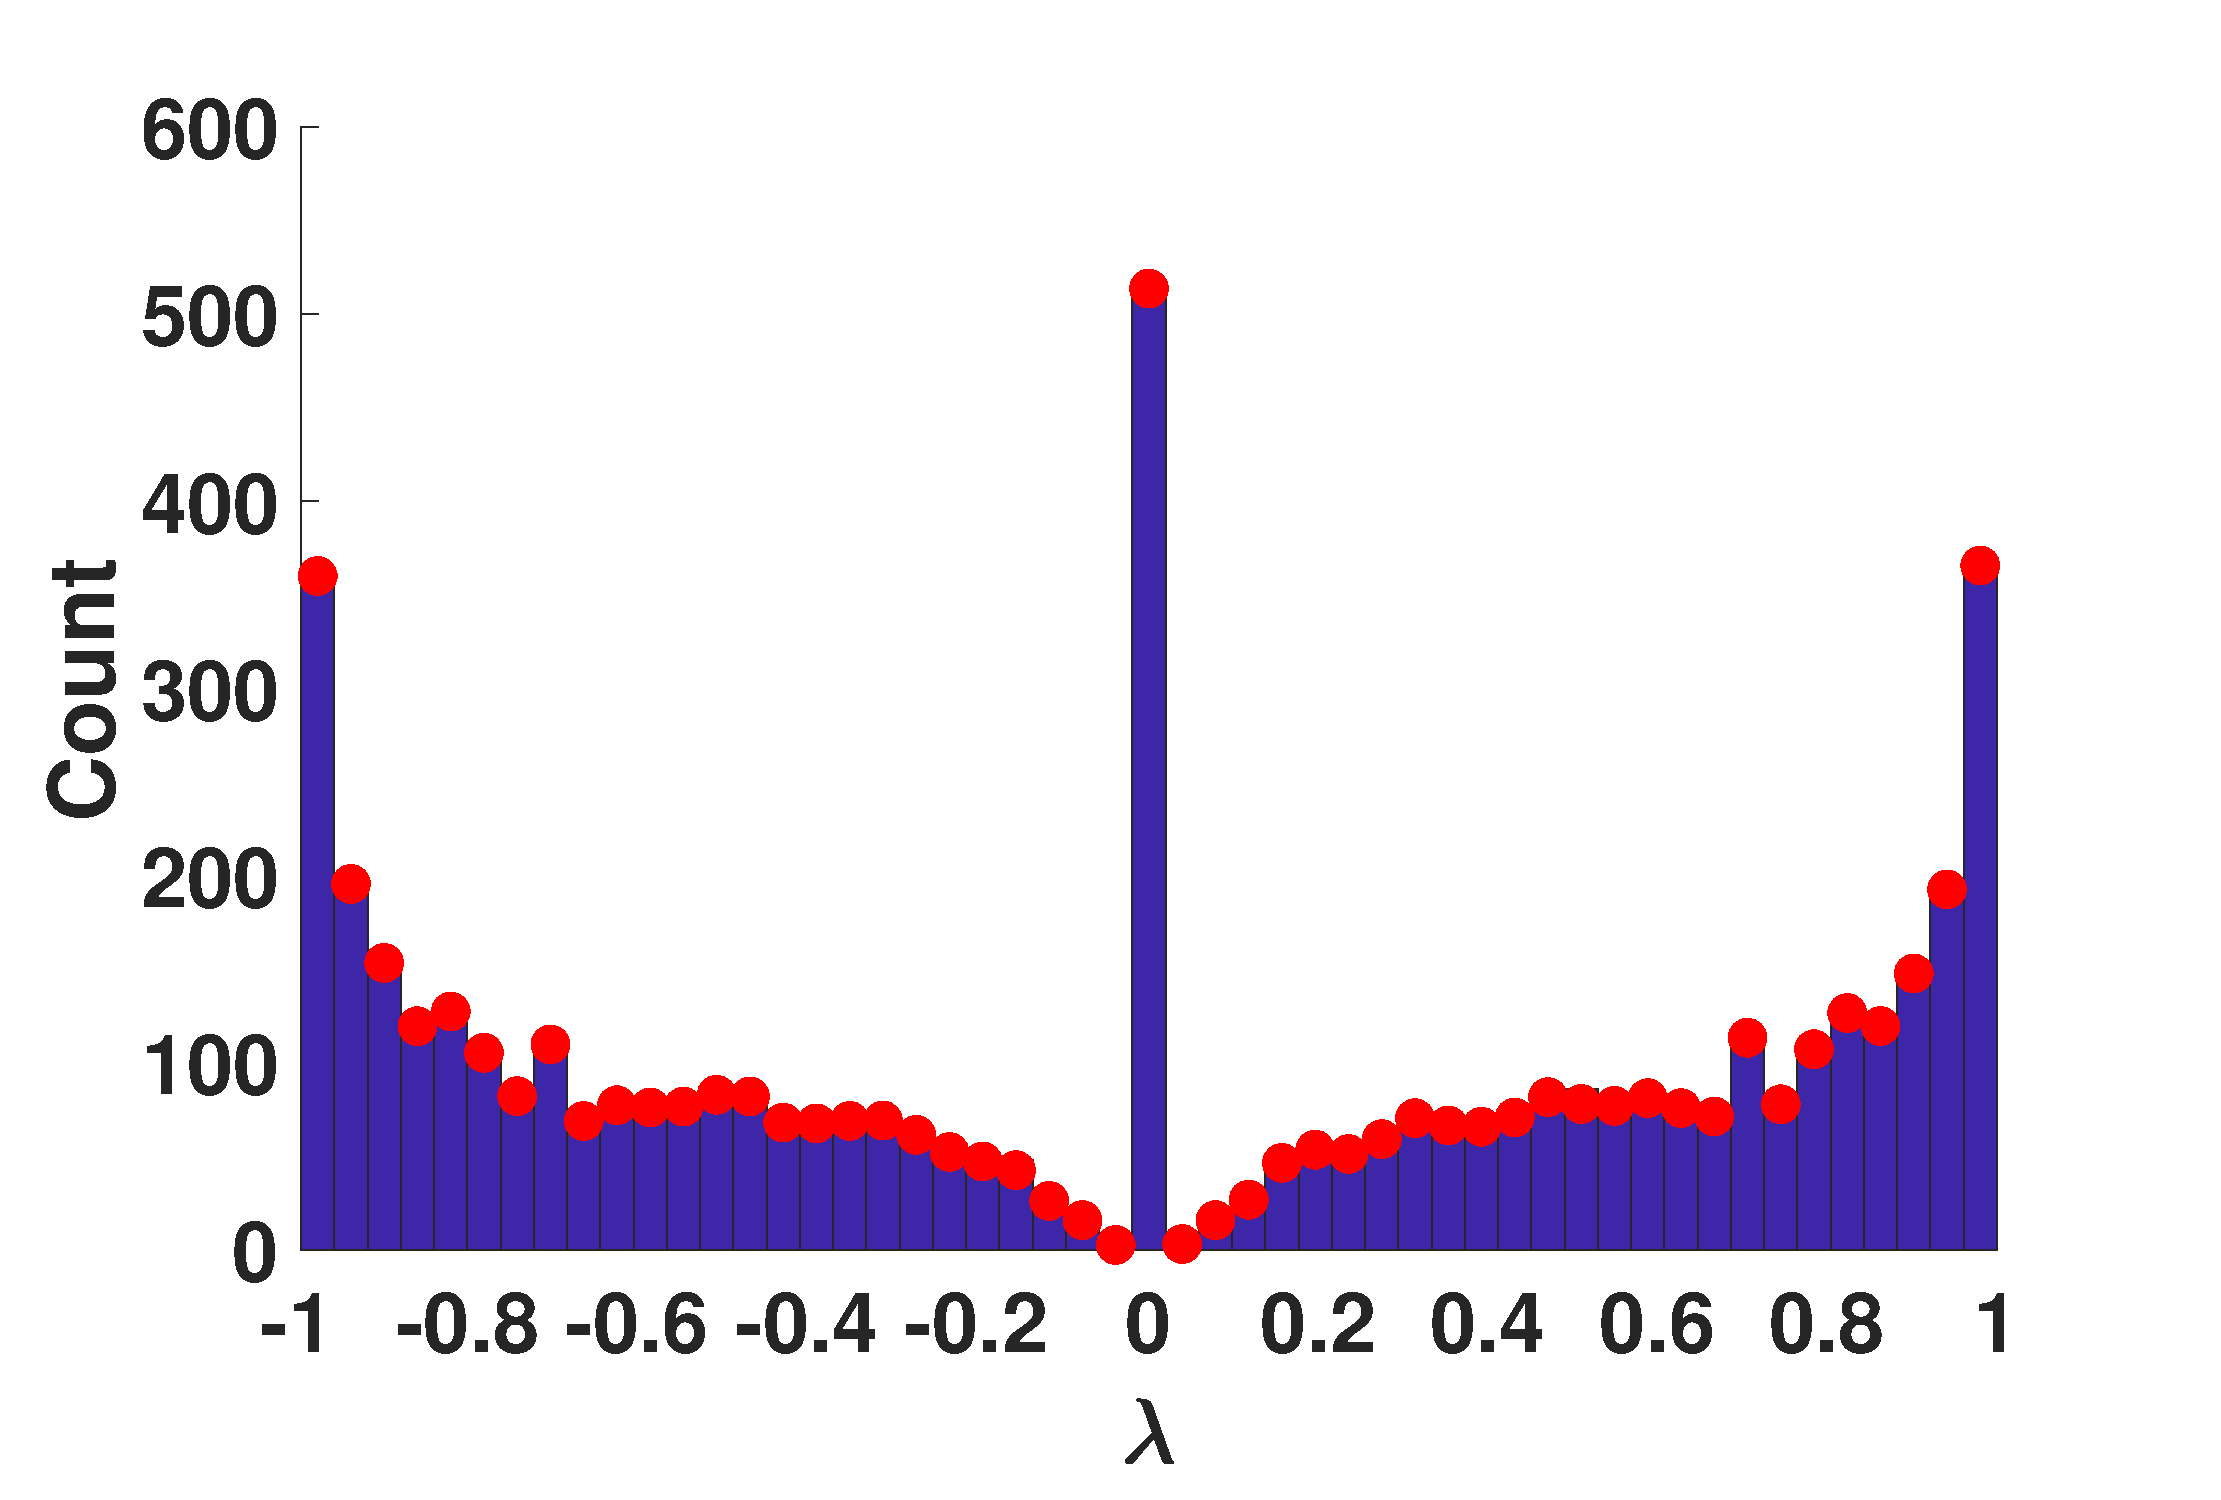
\includegraphics[width=\textwidth,trim = .4cm 0.5cm 3.5cm 1.3cm,clip]
    {./ndos/pics/sw_sparse}
    \caption{$\abs{E}=5k$}\label{fig:sw_sparse}
  \end{subfigure}
  %
  \begin{subfigure}{0.47\textwidth}
    \centering
    \captionsetup{justification=centering}
    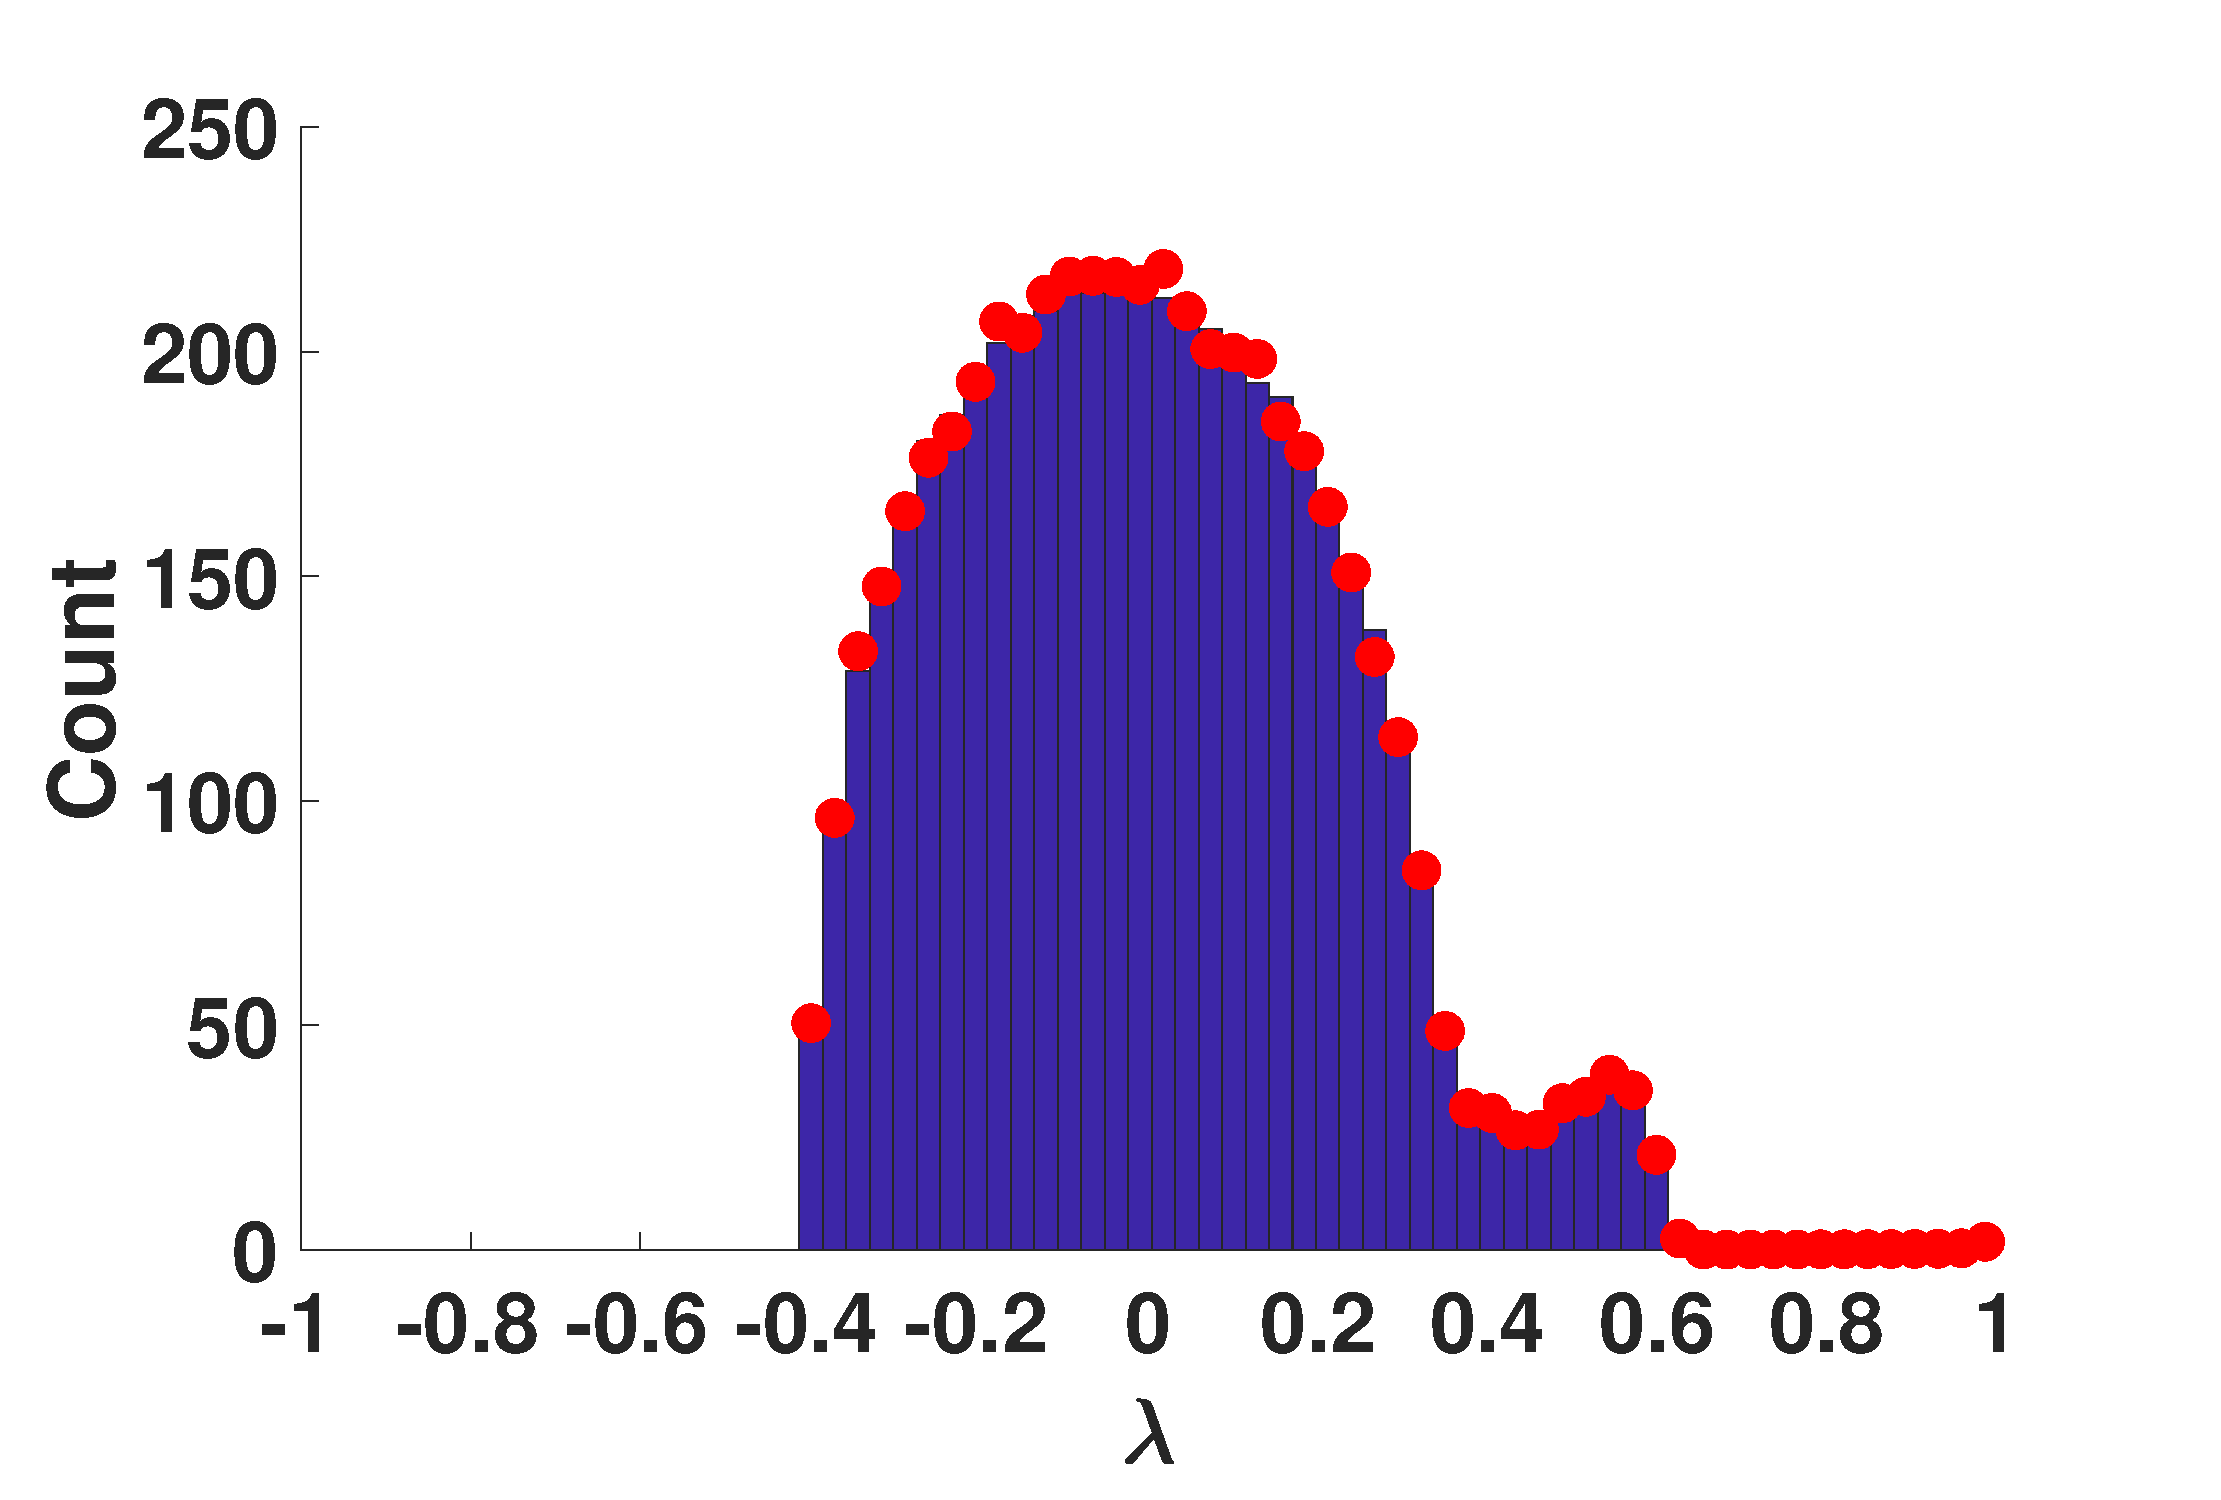
\includegraphics[width=\textwidth,trim = .4cm 0.5cm 3.5cm 1.3cm,clip]
    {./ndos/pics/sw_dense}
    \caption{$\abs{E}=50k$}\label{fig:sw_dense}
  \end{subfigure}
  \caption{Spectral histograms for small-world model with $5000$ nodes and
  re-wiring probability $p=0.5$, starting with $5000$ (\ref{fig:sw_sparse}) and
  $50000$ (\ref{fig:sw_dense} edges. Blue bars are the real spectrum, red points
  are from KPM ($5000$ moments and $20$ probes).} \label{fig:sw}
\end{figure}

Finally, we investigate the Block Two-Level \ErdosRenyi\ (BTER) model 
\cite{seshadhri2012community}, which directly fits an input graph. BTER
constructs a similar graph by a two-step process: first create a collection of
\ErdosRenyi\ subgraphs, then interconnect those using a Chung-Lu model  
\cite{chung2002connected}. \citeauthor{seshadhri2012community} showed their
model accurately captures the observable properties of the given graph,
including the eigenvalues of the adjacency matrix. \cref{fig:bter} compares the
DOS/PDOS of the Erd\"{o}s collaboration network and its BTER counterpart. Unlike
the original graph, most $0$ eigenvalues in BTER graph come from isolated nodes.
The BTER graph also has many more isolated edges ($\lambda=\pm1$),
singly-attached chains ($\lambda=\pm1/\sqrt{2})$), and singly-attached triangles
($\lambda=-1/2$). We locate these motifs by inspecting nodes with high weights
at respective part of the spectrum.

\begin{figure}[ht]
  \begin{subfigure}[t]{0.47\textwidth}
    \centering  
    \captionsetup{justification=centering}
    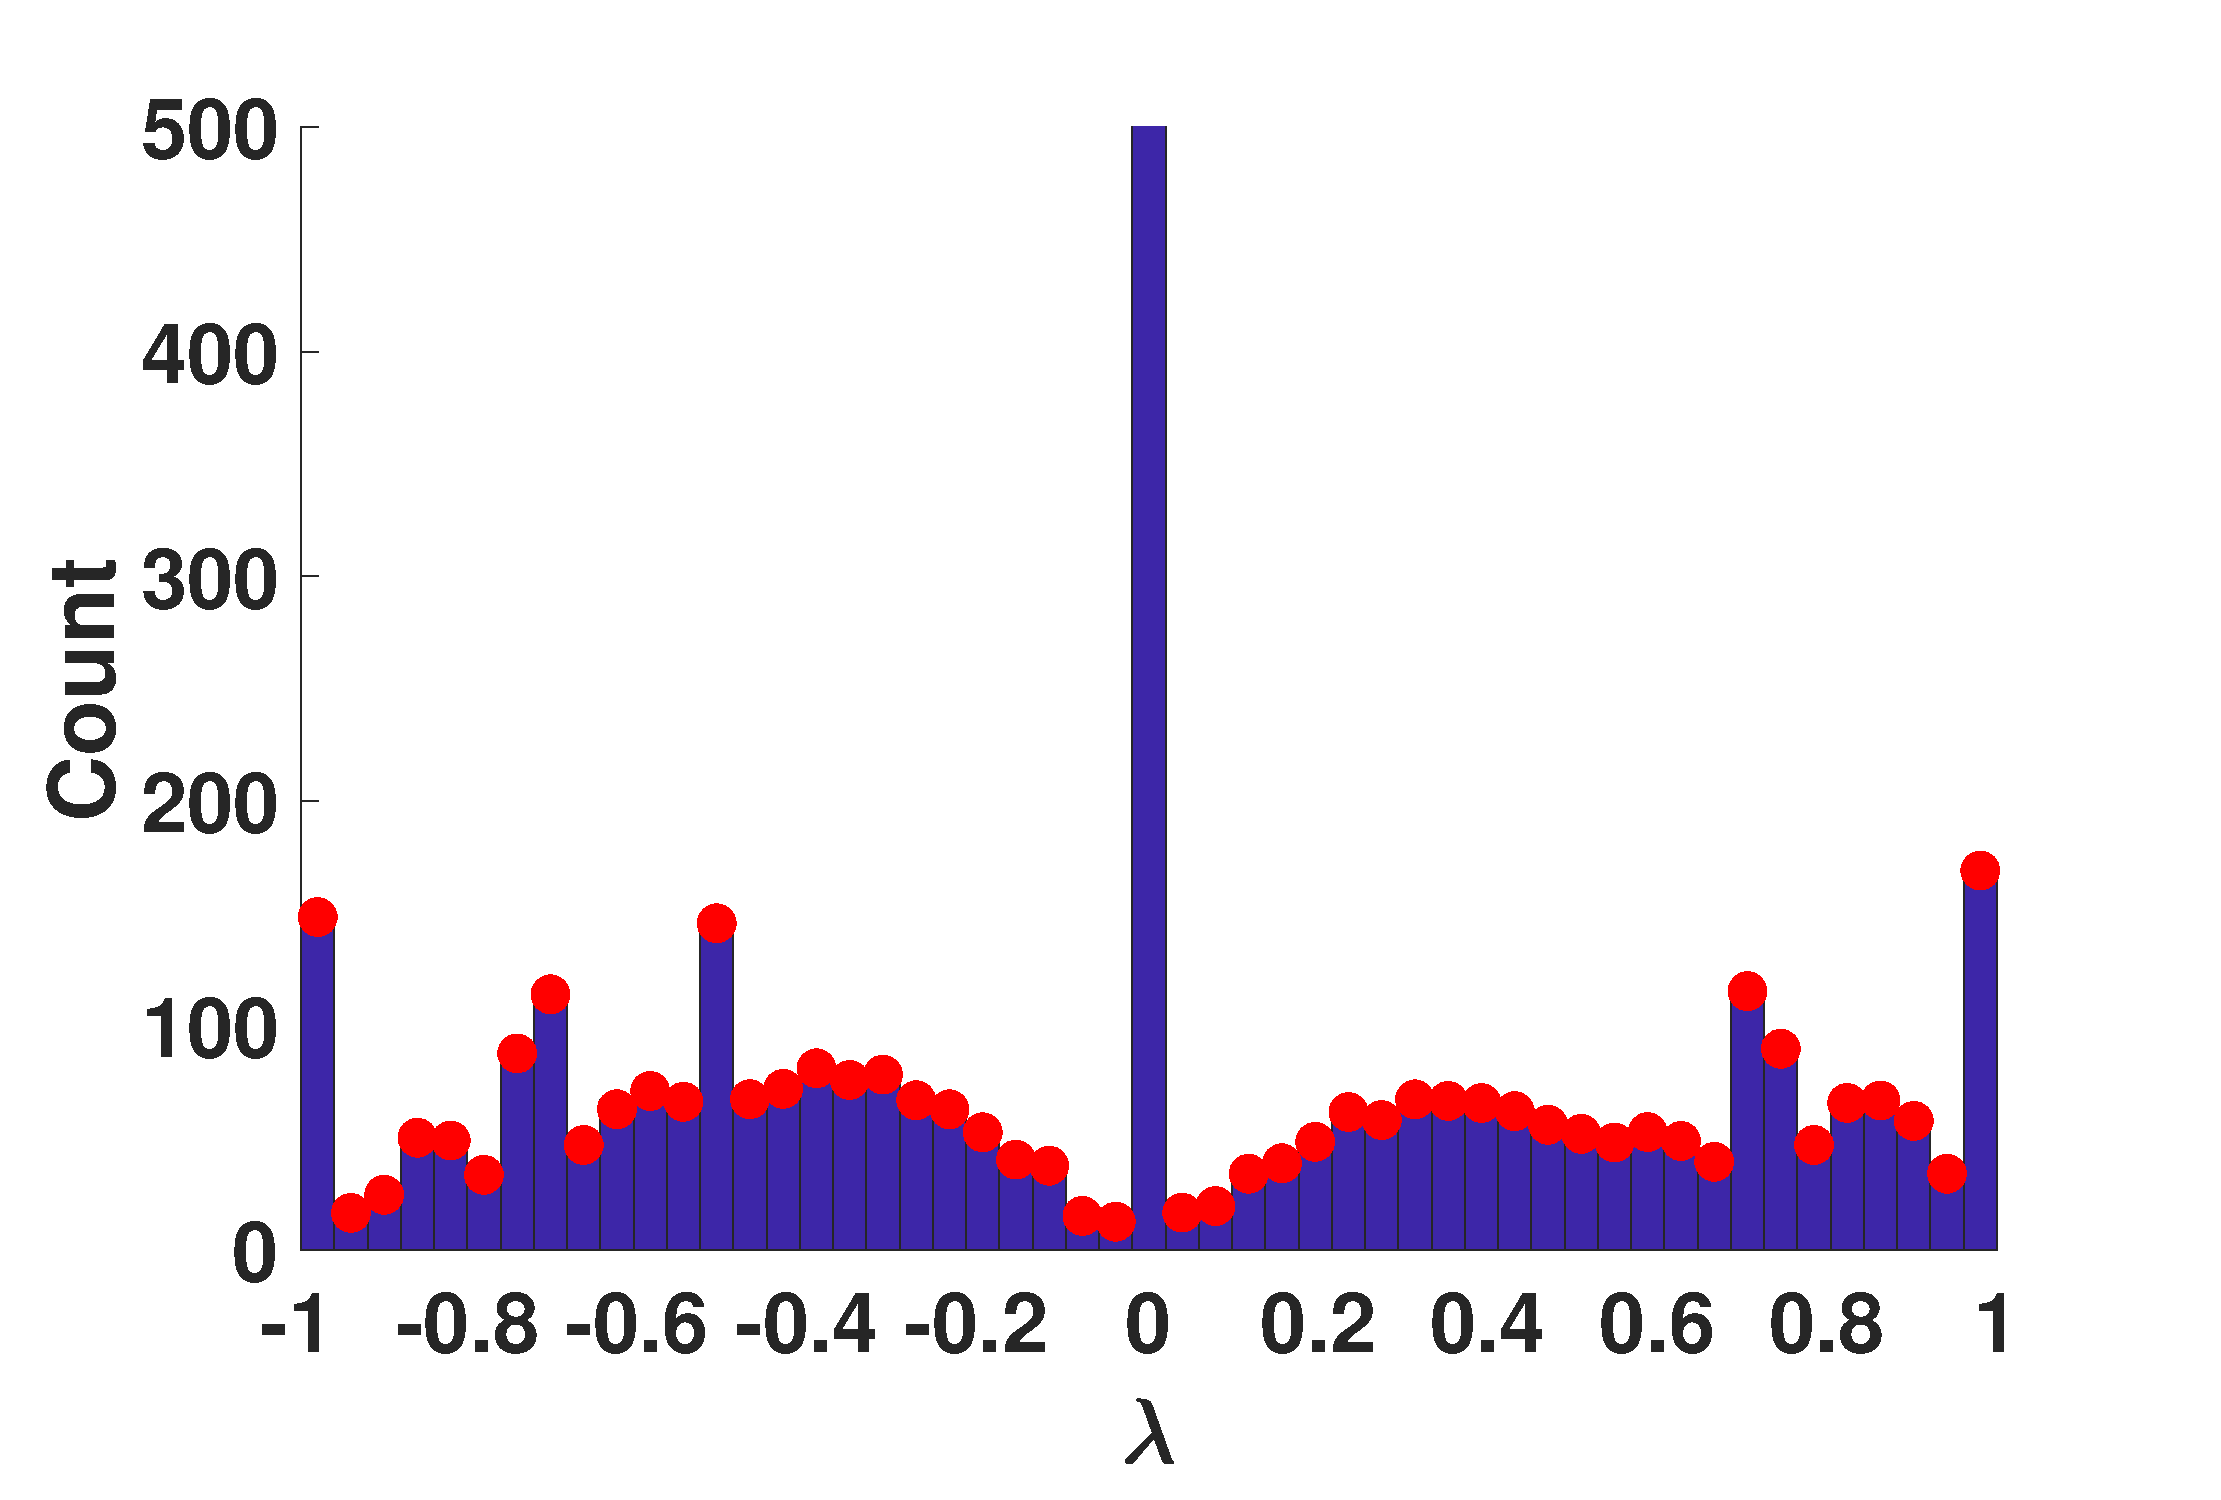
\includegraphics[width=\textwidth,trim = .4cm 0.5cm 3.5cm 1.3cm,clip]
    {./ndos/pics/bter_dos}
    \caption{BTER DOS}
    \label{fig:bter_dos}
  \end{subfigure}
  %
  \begin{subfigure}[t]{0.47\textwidth}
    \centering
    \captionsetup{justification=centering}
    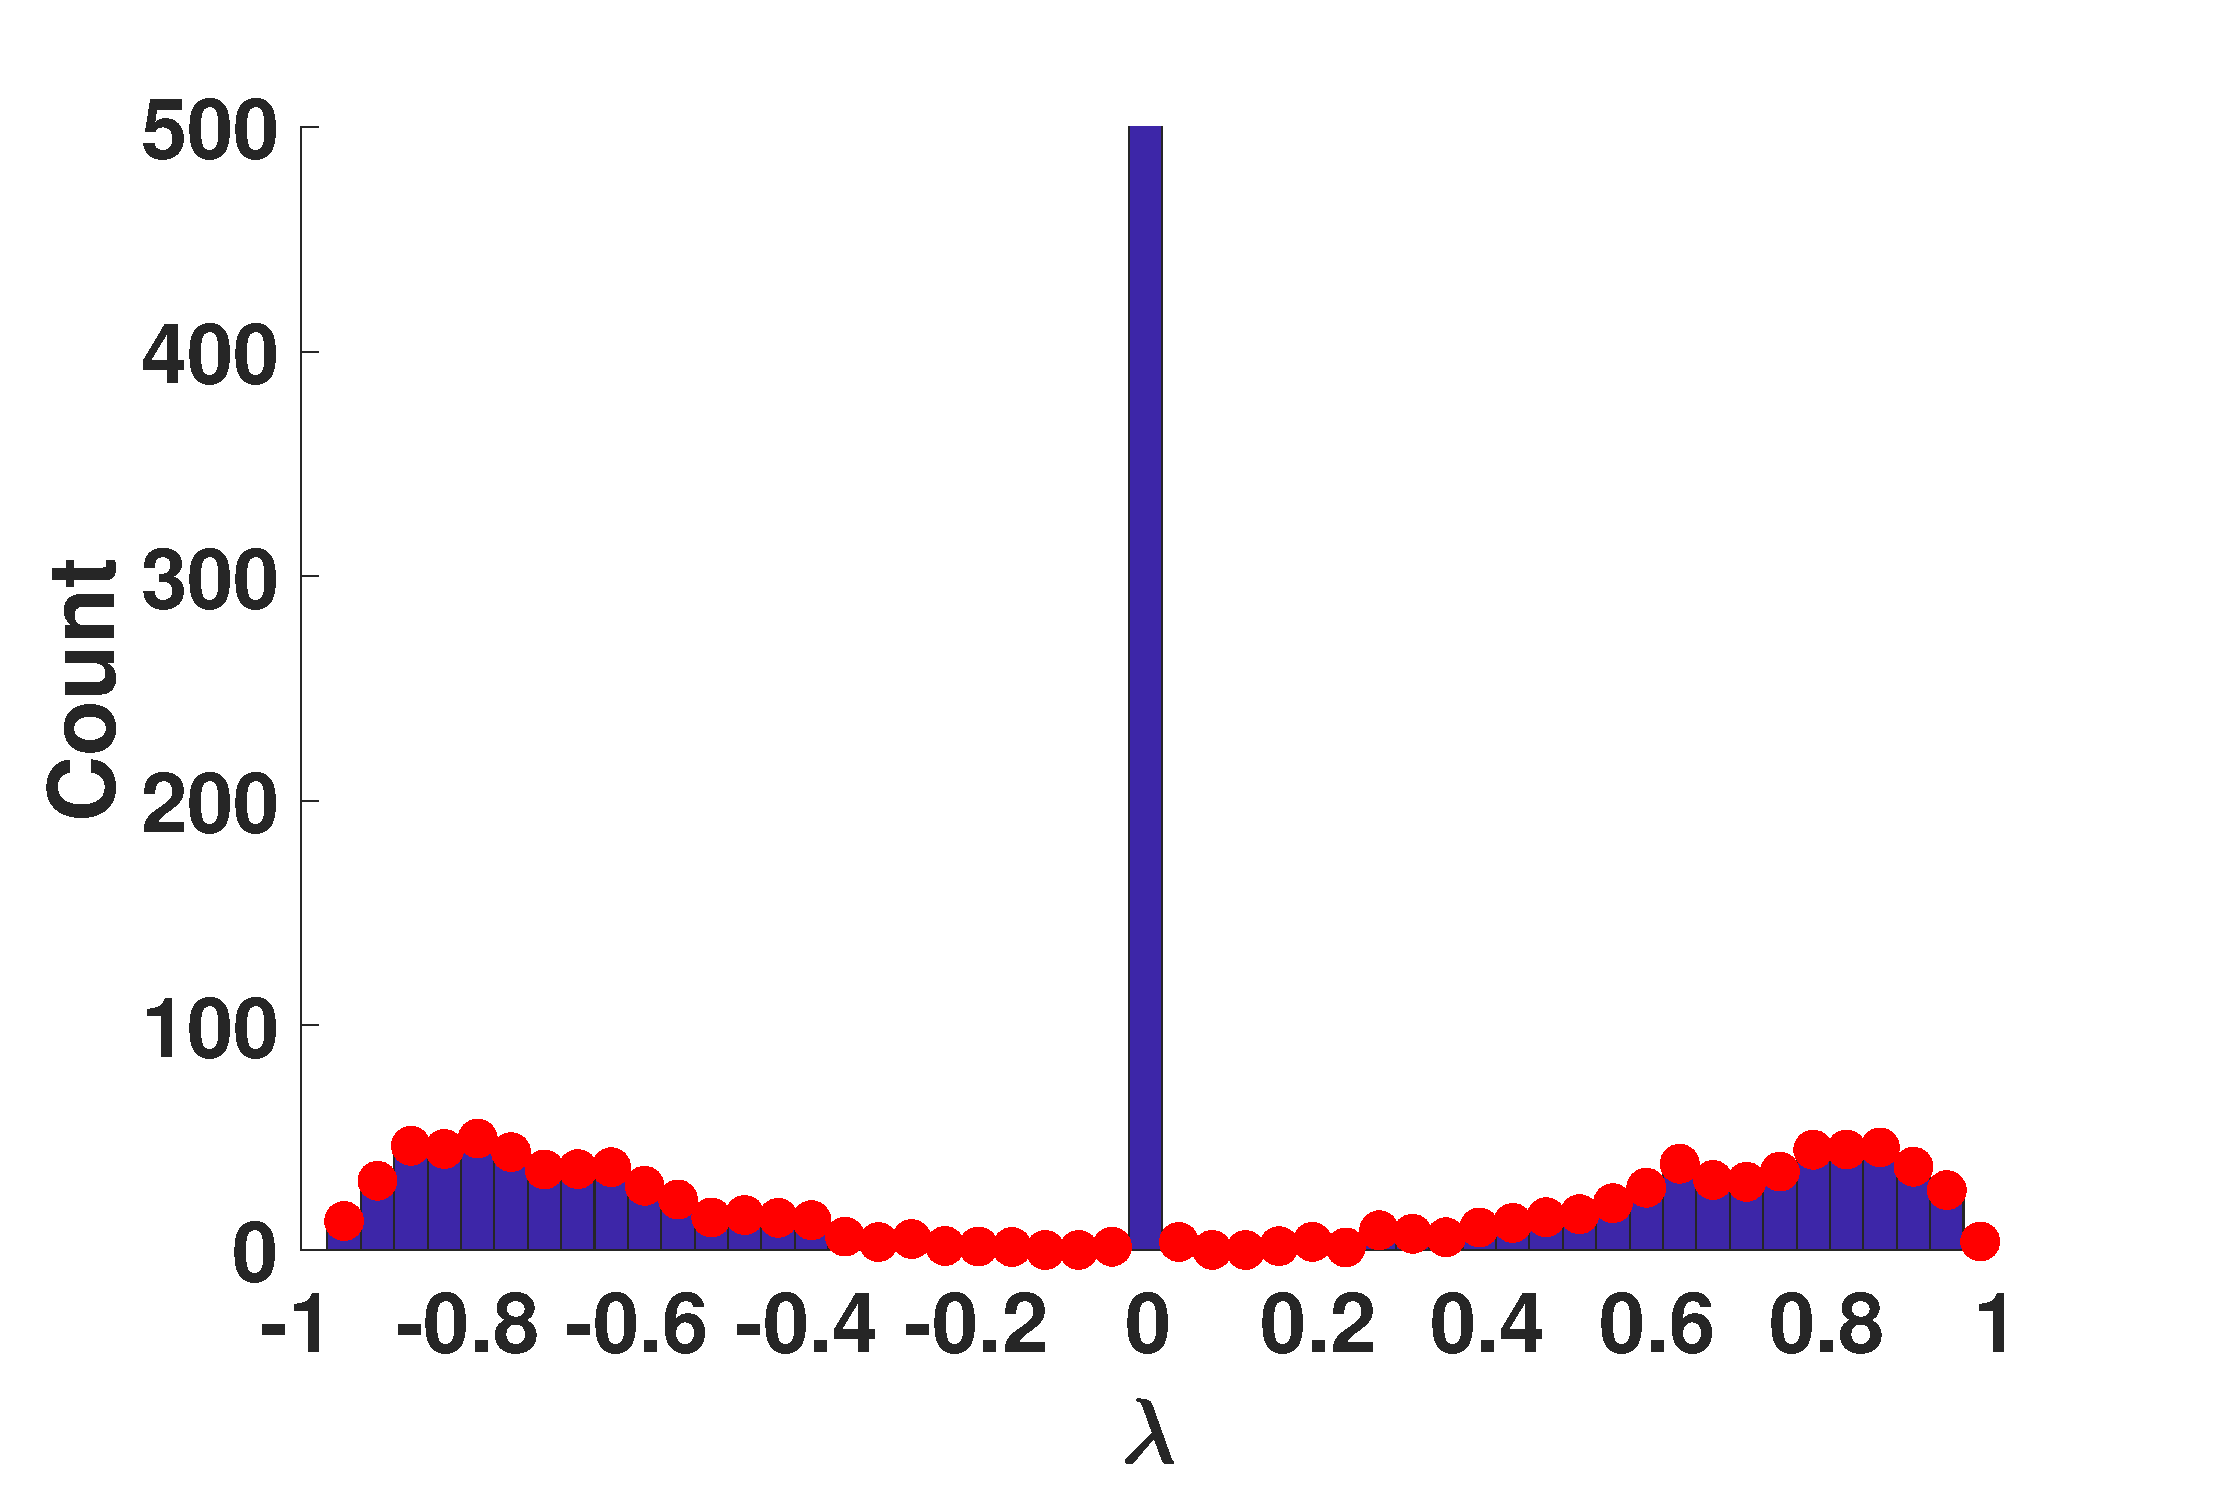
\includegraphics[width=\textwidth,trim = .4cm 0.5cm 3.5cm 1.3cm,clip]
    {./ndos/pics/erdos}
    \caption{\Erdos\ DOS}
    \label{fig:erdos_dos2}
  \end{subfigure}
  %
  \begin{subfigure}[t]{0.47\textwidth}
    \centering  
    \captionsetup{justification=centering}
    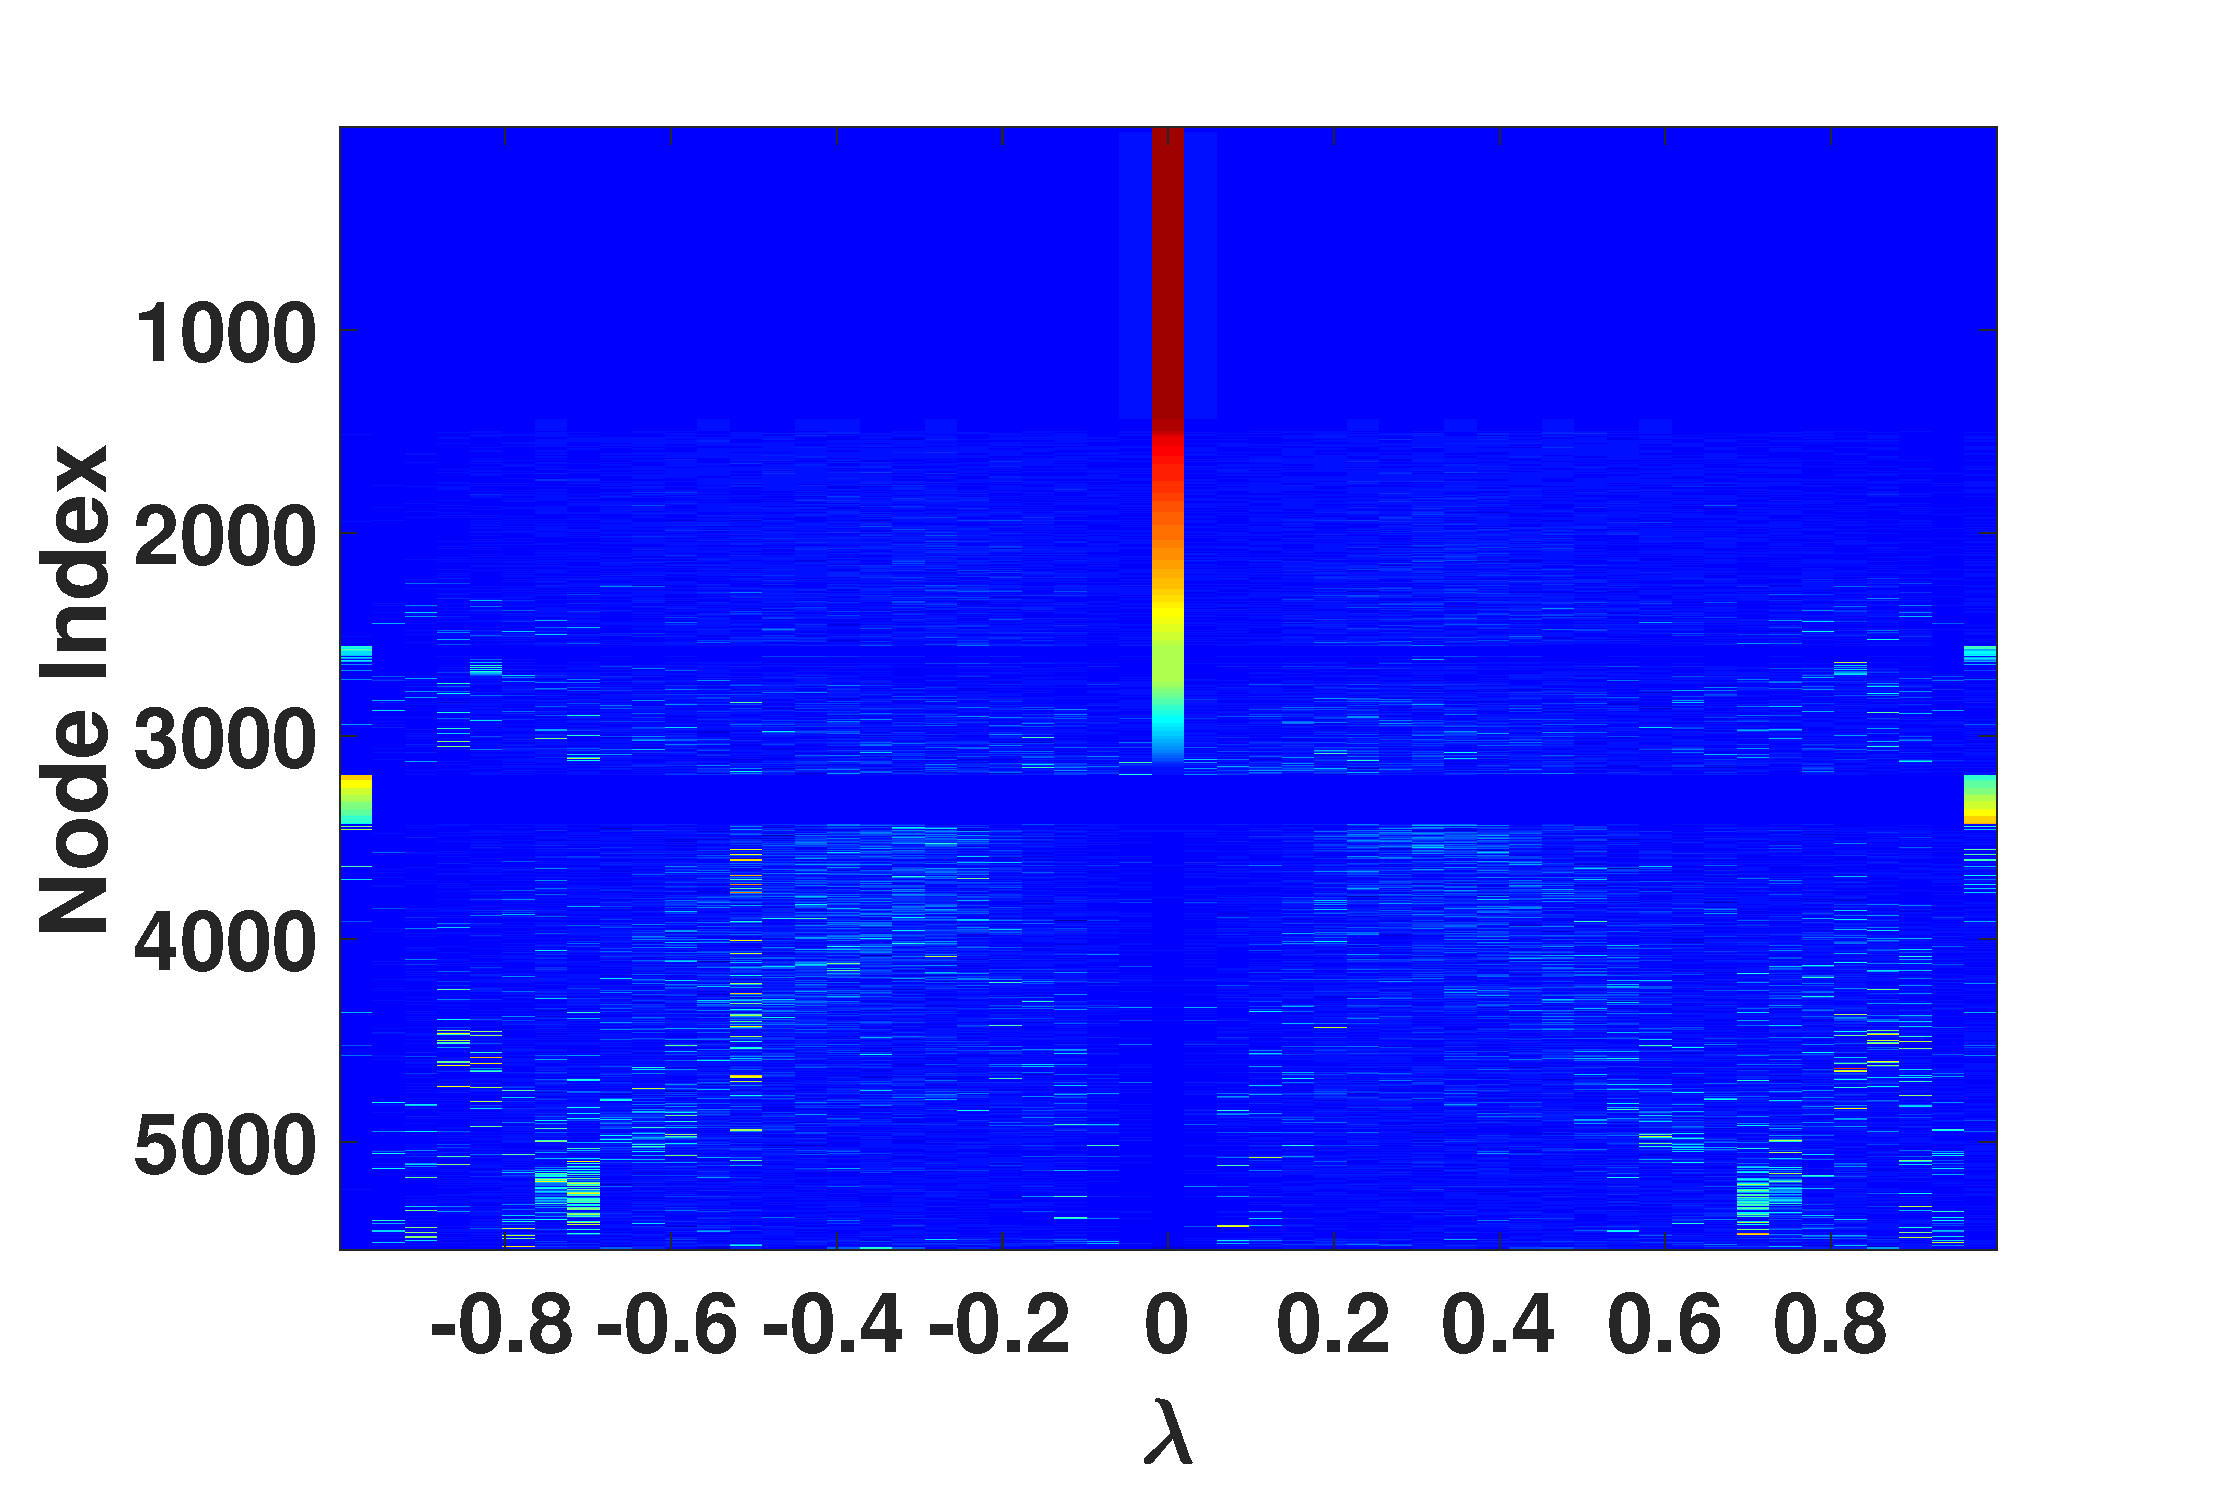
\includegraphics[width=\textwidth,trim = .4cm 0.5cm 3.5cm 1.3cm,clip]
    {./ndos/pics/bter_ldos}
    \caption{BTER PDOS}
    \label{fig:bter_ldos}
  \end{subfigure}
  \hspace{1cm}
  \begin{subfigure}[t]{0.47\textwidth}
    \centering
    \captionsetup{justification=centering}
    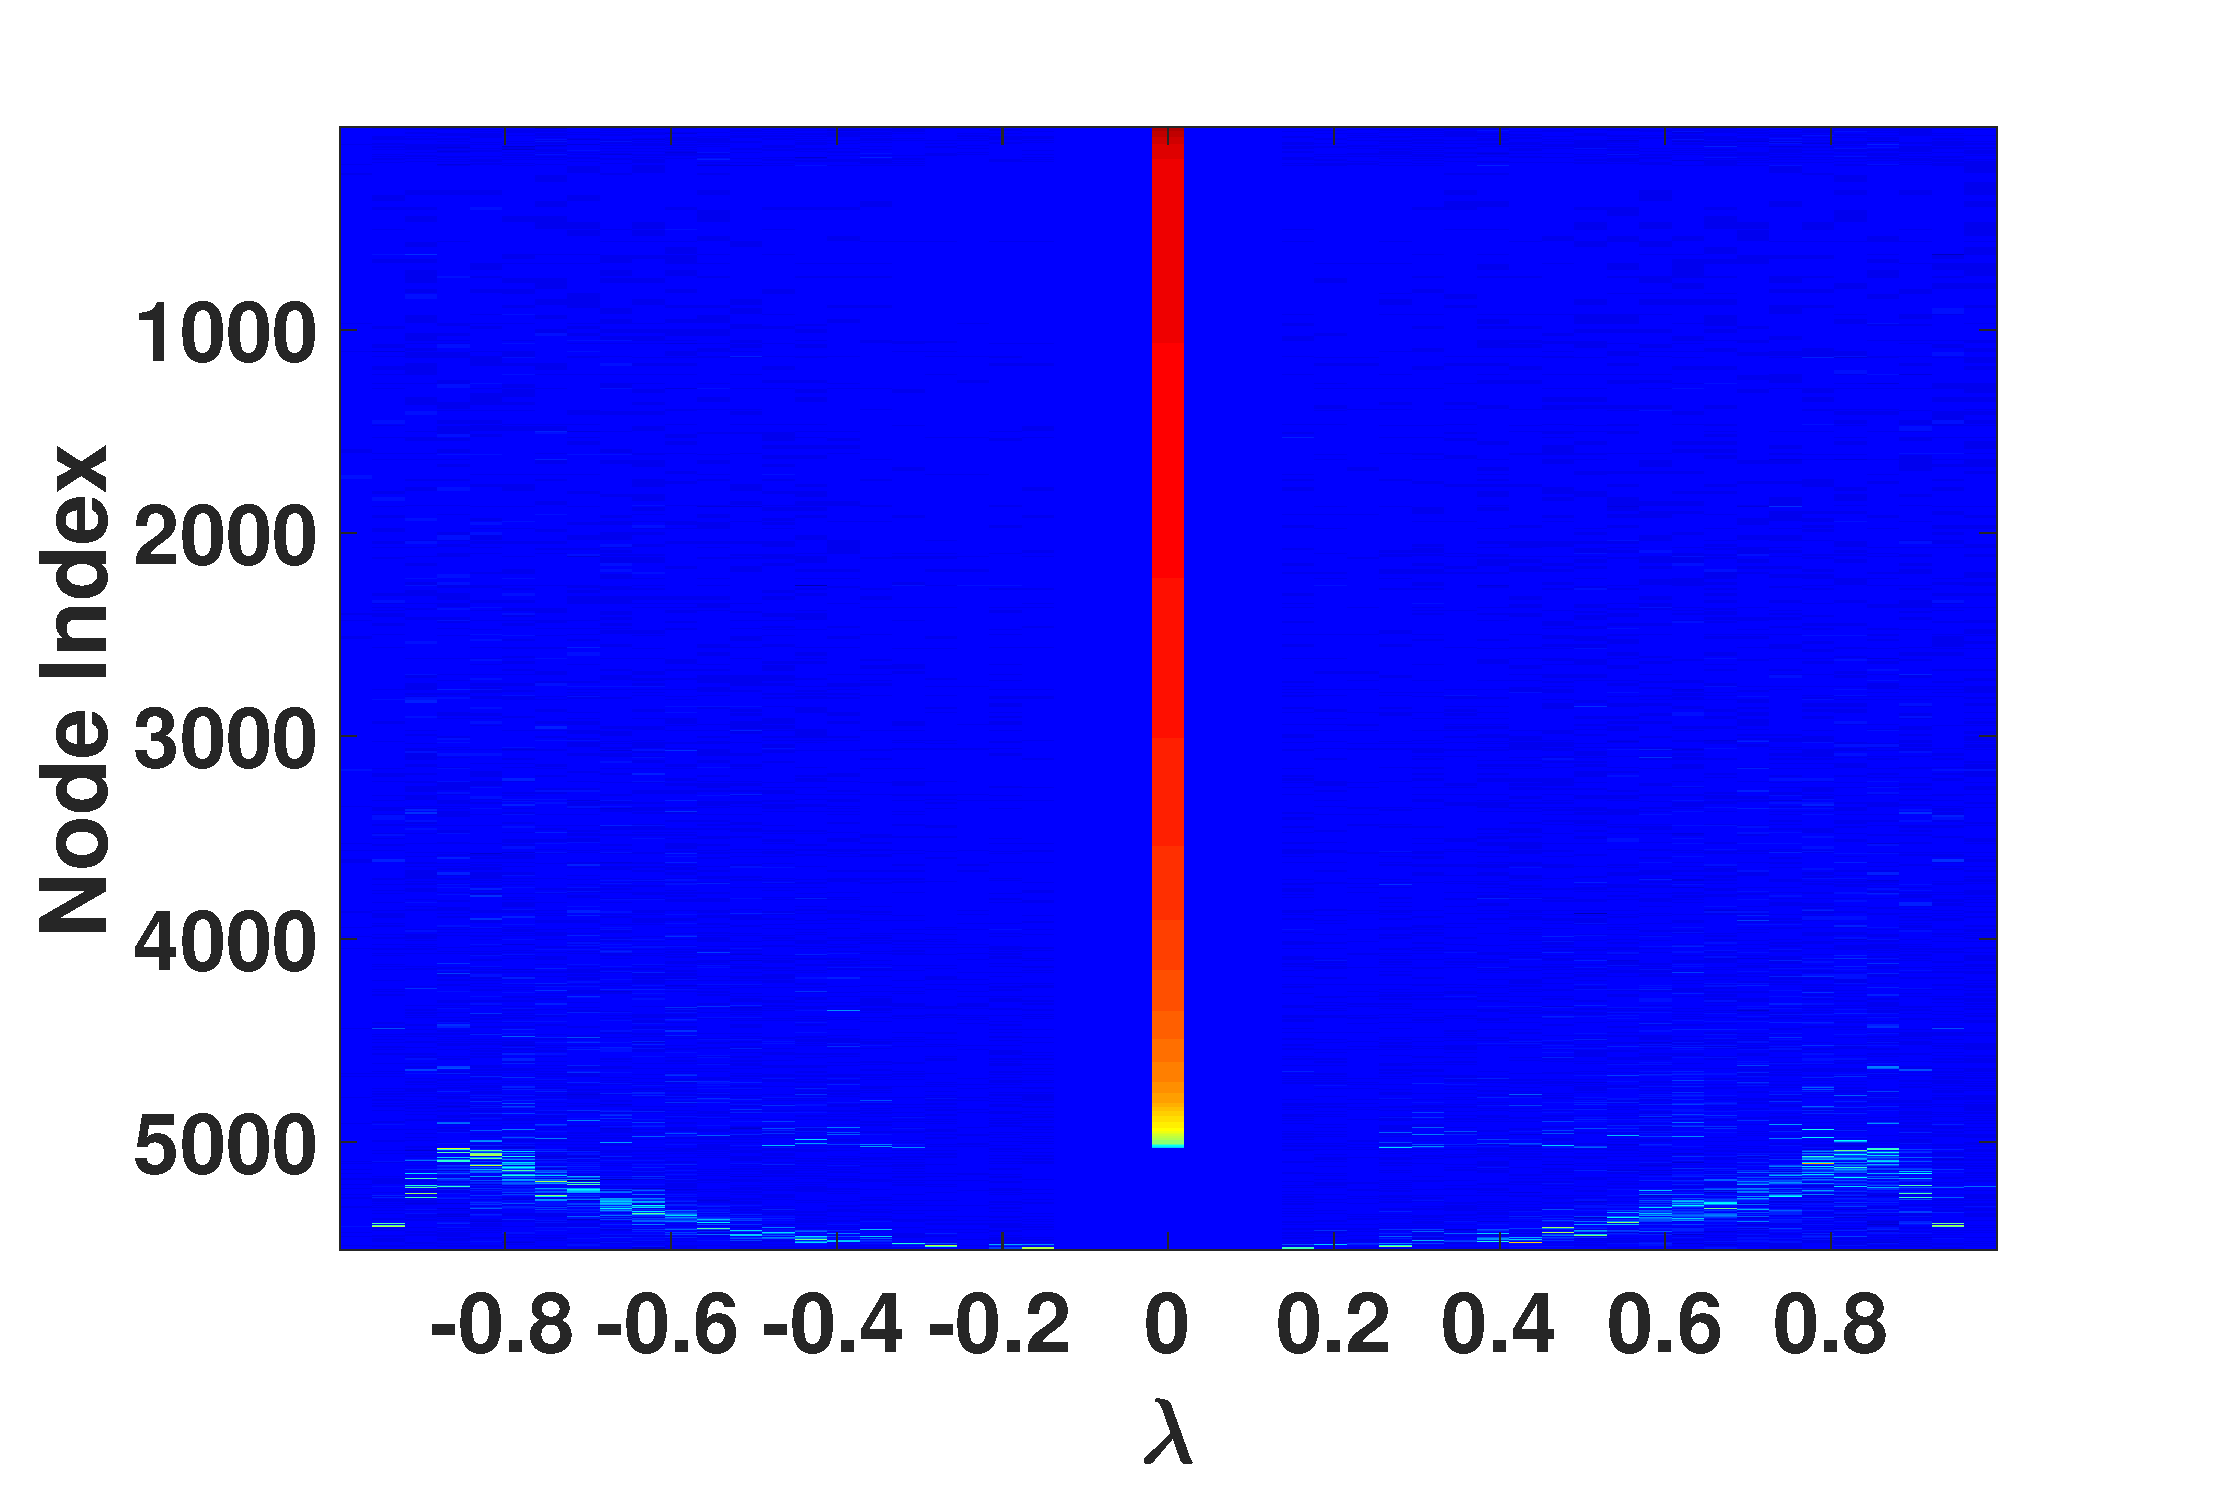
\includegraphics[width=\textwidth,trim = .4cm 0.5cm 3.5cm 1.3cm,clip]
    {./ndos/pics/erdos_ldos}
    \caption{\Erdos\ PDOS}
    \label{fig:erdos_ldos2}
  \end{subfigure}
  \caption{Comparison of spectral histogram between \Erdos\ Collaboration
  Network and the BTER model. Both DOS and PDOS are computed with $500$ moments
  and $20$ probe vectors.} \label{fig:bter}
\end{figure}